% Preambel mit Einstellungen importieren
% Document type and used packages
\documentclass[open=right, % Kapitel darf nur auf rechten Seite beginnen
    paper=A4,               % DIN-A4-Papier
    a4paper,                % DIN-A4-Papier
    12pt,                   % Schriftgöße
    headings=small,         % Kleine Überschriften
    headsepline=true,       % Trennlinie am Kopf der Seite
    footsepline=false,      % Keine Trennlinie am Fuß der Seite
    bibliography=totoc,     % Literaturverzeichnis in das Inhaltsverzeichnis aufnehmen
    twoside=on,             % Doppelseitiger Druck - auf off stellen für einseitig
    DIV=7,                  % Verhältnis der Ränder zum bedruckten Bereich
    chapterprefix=true,     % Kapitel x vor dem Kapitelnamen
    cleardoublepage=plain]{scrbook} 

% Pakete einbinden, die benötigt werden
\usepackage{scrpage2}
\usepackage{textcomp}
 
\usepackage[]{algorithm2e}
\usepackage[table,xcdraw]{xcolor}
\usepackage{tcolorbox}
\usepackage{enumitem}
\usepackage[nointegrals]{wasysym}
\tcbuselibrary{skins}
\usepackage{svg}
\usepackage{soul}
\usepackage{lipsum}
\usepackage[utf8]{inputenc}       % Dateien in UTF-8 benutzen
\usepackage[T1]{fontenc}          % Zeichenkodierung
\usepackage{graphicx}             % Bilder einbinden
\usepackage[ngerman,english]{babel}       % Deutsch und Englisch unterstützen
\usepackage{xcolor}               % Color support
\usepackage{amsmath}              % Matheamtische Formeln
\usepackage{amsfonts}             % Mathematische Zeichensätze
\usepackage{amssymb}              % Mathematische Symbole
\usepackage{float}                % Fließende Objekte (Tabellen, Grafiken etc.)
\usepackage{tabularx}                % Fließende Objekte (Tabellen, Grafiken etc.)
\usepackage{booktabs}             % Korrekter Tabellensatz
\usepackage[printonlyused]{acronym}  % Abkürzungsverzeichnis [nur verwendete Abkürzugen]
\usepackage{makeidx}              % Sachregister
\usepackage{listings}             % Source Code listings
\usepackage{listingsutf8}         % Listings in UTF8
\usepackage[hang,font={sf,footnotesize},labelfont={footnotesize,bf}]{caption} % Beschriftungen
\usepackage[scaled]{helvet}       % Schrift Helvetia laden
\usepackage[absolute]{textpos}	  % Absolute Textpositionen (für Deckblatt)
\usepackage{calc}                 % Berechnung von Positionen
\usepackage{blindtext}            % Blindtexte
\usepackage[bottom=40mm,left=35mm,right=35mm,top=30mm]{geometry} % Ränder ändern
\usepackage{setspace}             % Abstände korrigieren
\usepackage{ifthen}               % Logische Bedingungen mit ifthenelse
\usepackage{scrhack}              % Get rid of tocbasic warnings
\usepackage[pagebackref=false]{hyperref}  % Hyperlinks
\usepackage[all]{hypcap}          % Korrekte Verlinkung von Floats
\usepackage[autostyle=true,german=quotes]{csquotes}   % Zitate
\usepackage{tikz}
\usepackage{subcaption}
\usetikzlibrary{shapes, shapes, arrows, positioning,calc}
\usepackage[]{algorithm2e}
\usepackage[backend=biber,
  isbn=false,                     % ISBN nicht anzeigen, gleiches geht mit nahezu allen anderen Feldern
  sortlocale=de_DE,               % Sortierung der Einträge für Deutsch
  %sortlocale=en_US,              % Sortierung der Einträge für Englisch
  autocite=inline,                % regelt Aussehen für \autocite (inline=\parancite)
  hyperref=true,                  % Hyperlinks für Ziate
  style=ieee                     % Zitate als Zahlen [1]
  %style=alphabetic               % Zitate als Kürzel und Jahr [Ein05]
  %style=authoryear                % Zitate Author und Jahr [Einstein (1905)]
]{biblatex}                       % Literaturverwaltung mit BibLaTeX
\usepackage{rotating}             % Seiten drehen

\setlength{\bibitemsep}{1em}     % Abstand zwischen den Literaturangaben
\setlength{\bibhang}{2em}        % Einzug nach jeweils erster Zeile

% Trennung von URLs im Literaturverzeichnis (große Werte [> 10000] verhindern die Trennung)
\defcounter{biburlnumpenalty}{10} % Strafe für Trennung in URL nach Zahl
\defcounter{biburlucpenalty}{500}  % Strafe für Trennung in URL nach Großbuchstaben
\defcounter{biburllcpenalty}{500}  % Strafe für Trennung in URL nach Kleinbuchstaben

% Farben definieren
\definecolor{linkblue}{RGB}{0, 0, 100}
\definecolor{linkblack}{RGB}{0, 0, 0}
\definecolor{comment}{RGB}{63, 127, 95}
\definecolor{darkgreen}{RGB}{14, 144, 102}
\definecolor{darkblue}{RGB}{0,0,168}
\definecolor{darkred}{RGB}{128,0,0}
\definecolor{javadoccomment}{RGB}{0,0,240}
\definecolor{sensororange}{HTML}{FF9241}
\definecolor{aktorgreen}{HTML}{9FE1AE}
\definecolor{funcviolet}{HTML}{C68EEE}


% Einstellungen für das Hyperlink-Paket
\hypersetup{
    colorlinks=true,      % Farbige links verwenden       
%    allcolors=linkblue,
    linktoc=all,          % Links im Inhaltsverzeichnis
    linkcolor=linkblack,  % Querverweise
    citecolor=linkblack,  % Literaturangaben
	filecolor=linkblack,  % Dateilinks
	urlcolor=linkblack    % URLs
}

% Einstellungen für Quelltexte
\lstset{     
      xleftmargin=0.2cm,     
      basicstyle=\footnotesize\ttfamily,
      keywordstyle=\color{darkgreen},
      identifierstyle=\color{darkblue},
      commentstyle=\color{comment}, 
      stringstyle=\color{darkred}, 
      tabsize=2,
      lineskip={2pt},
      columns=flexible,
      inputencoding=utf8,
      captionpos=b,
      breakautoindent=true,
	  breakindent=2em,
	  breaklines=true,
	  prebreak=,
	  postbreak=,
      numbers=none,
      numberstyle=\tiny,
      showspaces=false,      % Keine Leerzeichensymbole
      showtabs=false,        % Keine Tabsymbole
      showstringspaces=false,% Leerzeichen in Strings
      morecomment=[s][\color{javadoccomment}]{/**}{*/},
      literate={Ö}{{\"O}}1 {Ä}{{\"A}}1 {Ü}{{\"U}}1 {ß}{{\ss}}2 {ü}{{\"u}}1 {ä}{{\"a}}1 {ö}{{\"o}}1
}

\urlstyle{same}

% Einstellungen für Überschriften
\renewcommand*{\chapterformat}{%
  \Large\chapapp~\thechapter   % Große Schrift
  \vspace{0.3cm}               % Abstand zum Titel des Kapitels
}

% Abstände für die Überschriften setzen
\renewcommand{\chapterheadstartvskip}{\vspace*{2.6cm}}
\renewcommand{\chapterheadendvskip}{\vspace*{1.5cm}}

\RedeclareSectionCommand[
  beforeskip=-1.8\baselineskip,
  afterskip=0.25\baselineskip]{section}

\RedeclareSectionCommand[
  beforeskip=-1.8\baselineskip,
  afterskip=0.15\baselineskip]{subsection}

\RedeclareSectionCommand[
  beforeskip=-1.8\baselineskip,
  afterskip=0.15\baselineskip]{subsubsection}


% In der Kopfzeile nur die kurze Kapitelbezeichnung (ohne Kapitel davor)
\renewcommand*\chaptermarkformat{\thechapter\autodot\enskip}
\automark[chapter]{chapter}

% Einstellungen für Schriftarten
\setkomafont{pagehead}{\normalfont\sffamily}
\setkomafont{pagenumber}{\normalfont\sffamily}
\setkomafont{paragraph}{\sffamily\bfseries\small}
\setkomafont{subsubsection}{\sffamily\itshape\bfseries\small}
\addtokomafont{footnote}{\footnotesize}
\setkomafont{chapter}{\LARGE\selectfont\bfseries}

% Wichtige Abstände
\setlength{\parskip}{0.2cm}  % 2mm Abstand zwischen zwei Absätzen
\setlength{\parindent}{0mm}  % Absätze nicht einziehen
\clubpenalty = 10000         % Keine "Schusterjungen"
\widowpenalty = 10000        % Keine "Hurenkinder"
\displaywidowpenalty = 10000 % Keine "Hurenkinder"
\renewcommand{\footnotesize}{\fontsize{9}{10}\selectfont} % Größe der Fußnoten
\setlength{\footnotesep}{8pt} % Abstand zwischen den Fußnoten

% Index erzeugen
\makeindex

% Einfacher Font-Wechsel über dieses Makro
\newcommand{\changefont}[3]{
\fontfamily{#1} \fontseries{#2} \fontshape{#3} \selectfont}

% Eigenes Makro für Bilder
\newcommand{\bild}[3]{
\begin{figure}[h]
  \centering
  \includegraphics[width=#2]{#1}
  \caption{#3}
  \label{#1}
\end{figure}}

% Wo liegt Sourcecode?
\newcommand{\srcloc}{src/}

% Wo sind die Bilder?
\graphicspath{{bilder/}}

% Makros für typographisch korrekte Abkürzungen
\newcommand{\zb}[0]{z.\,B.\ }
\newcommand{\dahe}[0]{d.\,h.\ }
\newcommand{\ua}[0]{u.\,a.\ }

% Flags für Veröffentlichung und Sperrvermerk
\newboolean{hsmapublizieren}
\newboolean{hsmasperrvermerk}


% for adjustwidth environment
\usepackage[strict]{changepage}

% for formal definitions
\usepackage{framed}

% environment derived from framed.sty: see leftbar environment definition
\definecolor{formalshade}{rgb}{0.95,0.95,1}

\newenvironment{formal}{%
  \def\FrameCommand{%
    \hspace{1pt}%
    {\color{darkblue}\vrule width 2pt}%
    {\color{formalshade}\vrule width 4pt}%
    \colorbox{formalshade}%
  }%
  \MakeFramed{\advance\hsize-\width\FrameRestore}%
  \noindent\hspace{-4.55pt}% disable indenting first paragraph
  \begin{adjustwidth}{}{7pt}%
  \vspace{2pt}\vspace{2pt}%
}
{%
  \vspace{2pt}\end{adjustwidth}\endMakeFramed%
}

% Dokumenteninfos importieren
% -------------------------------------------------------
% Daten für die Arbeit
% Wenn hier alles korrekt eingetragen wurde, wird das Titelblatt
% automatisch generiert. D.h. die Datei titelblatt.tex muss nicht mehr
% angepasst werden.

\newcommand{\hsmasprache}{de} % de oder en für Deutsch oder Englisch
                              % Für korrekt sortierte Literatureinträge, noch preambel.tex anpassen

% Titel der Arbeit auf Deutsch
\newcommand{\hsmatitelde}{flowws: eine End-User Development Schnittstelle zur Prototypisierung von IoT Systemen}

% Titel der Arbeit auf Englisch
\newcommand{\hsmatitelen}{flowws: an End-User Development Interface for prototyping IoT-Solutions}

% Weitere Informationen zur Arbeit
\newcommand{\hsmaort}{Mannheim}    % Ort
\newcommand{\hsmaautorvname}{Christoph} % Vorname(n)
\newcommand{\hsmaautornname}{Brutscher} % Nachname(n)
\newcommand{\hsmadatum}{xx.xx.2018} % Datum der Abgabe
\newcommand{\hsmajahr}{2018} % Jahr der Abgabe
\newcommand{\hsmafirma}{CAS Software GmbH, Karlsruhe} % Firma bei der die Arbeit durchgeführt wurde
\newcommand{\hsmabetreuer}{Prof. Kirstin Kohler, Hochschule Mannheim} % Betreuer an der Hochschule
\newcommand{\hsmazweitkorrektor}{Prof. Peter Kaiser, Hochschule Mannheim} % Betreuer im Unternehmen oder Zweitkorrektor
\newcommand{\hsmafakultaet}{I} % I für Informatik
\newcommand{\hsmastudiengang}{IM} % IB IMB UIB IM MTB

% Zustimmung zur Veröffentlichung
\setboolean{hsmapublizieren}{true}   % Einer Veröffentlichung wird zugestimmt
\setboolean{hsmasperrvermerk}{false} % Die Arbeit hat keinen Sperrvermerk

% -------------------------------------------------------
% Abstract

% Kurze (maximal halbseitige) Beschreibung, worum es in der Arbeit geht auf Deutsch
\newcommand{\hsmaabstractde}{
Diese Thesis handelt über die Konzeption eines \acl{EUD}-Werkzeuges, das Designer dabei unterstützen soll, schnell, flexibel und mit geringem Lernaufwand die Programmlogik von Prototypen im Bereich der \acl{IoT} zu entwickeln. 

Das Projekt cBlocks (''\textit{connected Blocks}'', siehe \cite{weckbach2018cblocks}) hat zum Ziel, die Erstellung von funktionalen Prototypen im Bereich \acs{IoT} zu erleichtern, indem es die elektrotechnische Komplexität kapselt und für den Endnutzer abstrahiert. Um \textit{Smart Objects}-Prototypen zu erstellen benötigt es allerdings noch eine weitere Komponente: Programmlogik. Das in dieser Thesis erarbeitete \acs{EUD}-Konzept (genannt ''\textit{flowws}''), nimmt sich diesem Problem an. 

Im Verlauf dieser Thesis werden die speziellen Bedürfnisse des Projektkontexts und der involvierten Stakeholder erhoben und analysiert. Auf Basis dieser Erhebung wird eine einzigartiges \acs{EUD}-Werkzeug konzeptioniert, welches auf einer Fusion von Datenfluss- und \acl{FSM}-Logik basiert. Es erlaubt Designern, graphisch Programmlogik zu erstellen und somit die verteilten cBlocks in \textit{Smart Objects} zusammenzuführen. Erste Nutzertests attestieren das Potential von flowws, eine gute Balance zwischen Ausdruckskomplexität und Erlernbarkeit gefunden zu haben.
}

% Kurze (maximal halbseitige) Beschreibung, worum es in der Arbeit geht auf Englisch

\newcommand{\hsmaabstracten}{
The goal of this thesis is the conception of an \acl{EUD}-Tool. This tool aids designers in the creation of \acl{IoT} prototypes by allowing them to program logic quickly ,flexibly and with little knowledge in coding.

The cBlocks-project (''\textit{connected Blocks}'', see \cite{weckbach2018cblocks}) defines a tool with the goal in mind to reduce the required electrotechnical knowledge in order to create \acs{IoT}-prototypes. It does so by encapsulating the technical complexities and thereby abstracting in a way that the enduser (i.e. the designer) can use them effortlessly. However, there is more to a smart device than electronics -- there is logic. Eleviating this problem is the goal the \ac{EUD}-Concept described this thesis.

In the course of this paper the needs of the project's (technical and functional) context and the needs of the stakeholder will be elaborated and analysed. This analysis will culminate in a \acs{EUD}-Tool which is resting on a unique fusion of Dataflow and \acl{FSM} based programming logic. This tool allows designers to graphically create programs which bind the distributed cBlocks together into \textit{Smart Objects}. A user test reveals flowws' potential to balance the expressiveness and learnability to fit the endusers' needs.

}


% Literatur-Datenbank
\addbibresource{literatur.bib}   % BibLaTeX-Datei mit Literaturquellen einbinden



\begin{document}

\frontmatter

% Römische Ziffern für die "Front-Matter"
\setcounter{page}{0}
\changefont{ptm}{m}{n}  % Times New Roman für den Fließtext
\renewcommand{\rmdefault}{ptm}

% Titelblatt
% -------------------------------------------------------
% In dieser Datei sollten eigentlich keine Veränderungen mehr
% notwendig sein.
% -------------------------------------------------------

\thispagestyle{empty}

% Fakultäten der HS-Mannheim
% -------------------------------------------------------
\ifthenelse{\equal{\hsmafakultaet}{I}}%
  {\newcommand{\hsmafakultaetlangde}{Fakultät für Informatik}%
   \newcommand{\hsmafakultaetlangen}{Department of Computer Science}}{}

\ifthenelse{\equal{\hsmafakultaet}{E}}%
  {\newcommand{\hsmafakultaetlangde}{Fakultät für Elektrotechnik}%
   \newcommand{\hsmafakultaetlangen}{Department of Electrical Engineering}}{}

\ifthenelse{\equal{\hsmafakultaet}{S}}%
  {\newcommand{\hsmafakultaetlangde}{Fakultät für Sozialwesen}%
   \newcommand{\hsmafakultaetlangen}{Department of Social Work}}{}
   
\ifthenelse{\equal{\hsmafakultaet}{B}}%
  {\newcommand{\hsmafakultaetlangde}{Fakultät für Biotechnologie}%
   \newcommand{\hsmafakultaetlangen}{Department of Biotechnology}}{}

\ifthenelse{\equal{\hsmafakultaet}{D}}%
  {\newcommand{\hsmafakultaetlangde}{Fakultät für Gestaltung}%
   \newcommand{\hsmafakultaetlangen}{Department of Design}}{}

\ifthenelse{\equal{\hsmafakultaet}{M}}%
  {\newcommand{\hsmafakultaetlangde}{Fakultät für Maschinenbau}%
   \newcommand{\hsmafakultaetlangen}{Department of Mechanical Engineering}}{}

\ifthenelse{\equal{\hsmafakultaet}{N}}%
  {\newcommand{\hsmafakultaetlangde}{Fakultät für Informationstechnik}%
   \newcommand{\hsmafakultaetlangen}{Department of Information Technology}}{}
   
\ifthenelse{\equal{\hsmafakultaet}{W}}%
  {\newcommand{\hsmafakultaetlangde}{Fakultät für Wirtschaftsingenieurwesen}%
   \newcommand{\hsmafakultaetlangen}{Department of Engineering and Management}}{}
   
\ifthenelse{\equal{\hsmafakultaet}{C}}%
  {\newcommand{\hsmafakultaetlangde}{Fakultät für Verfahrens- und Chemietechnik}%
   \newcommand{\hsmafakultaetlangen}{Department of Chemical Process Engineering}}{}
   

\ifthenelse{\equal{\hsmastudiengang}{IB}}%
  {\newcommand{\hsmastudienganglangde}{Informatik}%
  \newcommand{\hsmastudienganglangen}{Computer Science}%
  \newcommand{\hsmatypde}{Bachelor-Thesis}%
  \newcommand{\hsmatypen}{Bachelor Thesis}%
  \newcommand{\hsmagrad}{\hsmabsc}}{}

\ifthenelse{\equal{\hsmastudiengang}{IMB}}%
  {\newcommand{\hsmastudienganglangde}{Medizinische Informatik}%
  \newcommand{\hsmastudienganglangen}{Medical Informatics}%
  \newcommand{\hsmatypde}{Bachelor-Thesis}%
  \newcommand{\hsmatypen}{Bachelor Thesis}%
  \newcommand{\hsmagrad}{\hsmabsc}}{}
  
\ifthenelse{\equal{\hsmastudiengang}{UIB}}%
  {\newcommand{\hsmastudienganglangde}{Unternehmens- und Wirtschaftsinformatik}%
  \newcommand{\hsmastudienganglangen}{Enterprise Computing}%  
  \newcommand{\hsmatypde}{Bachelor-Thesis}%
  \newcommand{\hsmatypen}{Bachelor Thesis}%
  \newcommand{\hsmagrad}{\hsmabsc}}{}

\ifthenelse{\equal{\hsmastudiengang}{IM}}%
  {\newcommand{\hsmastudienganglangde}{Informatik}%
   \newcommand{\hsmastudienganglangen}{Computer Science}%
   \newcommand{\hsmatypde}{Master-Thesis}%
   \newcommand{\hsmatypen}{Master Thesis}%
   \newcommand{\hsmagrad}{\hsmamaster}}{}

\ifthenelse{\equal{\hsmastudiengang}{MEB}}%
  {\newcommand{\hsmastudienganglangde}{Mechatronik}%
   \newcommand{\hsmastudienganglangen}{Mechatronic}%
   \newcommand{\hsmatypde}{Bachelor-Thesis}%
   \newcommand{\hsmatypen}{Bachelor Thesis}%
   \newcommand{\hsmagrad}{\hsmabsc}}{}
   
\ifthenelse{\equal{\hsmastudiengang}{UB}}%
  {\newcommand{\hsmastudienganglangde}{Automatisierungstechnik}%
   \newcommand{\hsmastudienganglangen}{Automation Technology}%
   \newcommand{\hsmatypde}{Bachelor-Thesis}%
   \newcommand{\hsmatypen}{Bachelor Thesis}%
   \newcommand{\hsmagrad}{\hsmabsc}}{}
   
\ifthenelse{\equal{\hsmastudiengang}{ELB}}%
  {\newcommand{\hsmastudienganglangde}{Elektro- und Informationstechnik/Ingenieurpädagogik}%
   \newcommand{\hsmastudienganglangen}{Elektro- und Informationstechnik/Ingenieurpädagogik}%
   \newcommand{\hsmatypde}{Bachelor-Thesis}%
   \newcommand{\hsmatypen}{Bachelor Thesis}%
   \newcommand{\hsmagrad}{\hsmabsc}}{} 
   
\ifthenelse{\equal{\hsmastudiengang}{EBE}}%
  {\newcommand{\hsmastudienganglangde}{Energietechnik und erneuerbare Energien}%
   \newcommand{\hsmastudienganglangen}{Power Engineering ans Renewable Energies}%
   \newcommand{\hsmatypde}{Bachelor-Thesis}%
   \newcommand{\hsmatypen}{Bachelor Thesis}%
   \newcommand{\hsmagrad}{\hsmabsc}}{}

\ifthenelse{\equal{\hsmastudiengang}{TS}}%
  {\newcommand{\hsmastudienganglangde}{Translation Studies}%
   \newcommand{\hsmastudienganglangen}{Translation Studies}%
   \newcommand{\hsmatypde}{Bachelor-Thesis}%
   \newcommand{\hsmatypen}{Bachelor Thesis}%
   \newcommand{\hsmagrad}{\hsmabsc}}{}
  
\ifthenelse{\equal{\hsmastudiengang}{EM}}%
  {\newcommand{\hsmastudienganglangde}{Automatisierungs- und Energiesysteme}%
   \newcommand{\hsmastudienganglangen}{Automation and Energy Systems}%
   \newcommand{\hsmatypde}{Master-Thesis}%
   \newcommand{\hsmatypen}{Master Thesis}%
   \newcommand{\hsmagrad}{\hsmamaster}}{}
   
\ifthenelse{\equal{\hsmastudiengang}{ELM}}%
  {\newcommand{\hsmastudienganglangde}{Lehramt Ingenieurpädagogik}%
   \newcommand{\hsmastudienganglangen}{Lectureship Educational Engineering}%
   \newcommand{\hsmatypde}{Master-Thesis}%
   \newcommand{\hsmatypen}{Master Thesis}%
   \newcommand{\hsmagrad}{\hsmamaster}}{}
   
\ifthenelse{\equal{\hsmastudiengang}{SAB}}%
  {\newcommand{\hsmastudienganglangde}{Soziale Arbeit}%
   \newcommand{\hsmastudienganglangen}{Social Labour}%
   \newcommand{\hsmatypde}{Bachelor-Thesis}%
   \newcommand{\hsmatypen}{Bachelor Thesis}%
   \newcommand{\hsmagrad}{\hsmaba}}{}
   
\ifthenelse{\equal{\hsmastudiengang}{SAM}}%
  {\newcommand{\hsmastudienganglangde}{Soziale Arbeit}%
   \newcommand{\hsmastudienganglangen}{Social Labour}%
   \newcommand{\hsmatypde}{Master-Thesis}%
   \newcommand{\hsmatypen}{Master Thesis}%
   \newcommand{\hsmagrad}{\hsmamastera}}{}
   
\ifthenelse{\equal{\hsmastudiengang}{BB}}%
  {\newcommand{\hsmastudienganglangde}{Biotechnology}%
   \newcommand{\hsmastudienganglangen}{Biotechnology}%
   \newcommand{\hsmatypde}{Bachelor-Thesis}%
   \newcommand{\hsmatypen}{Bachelor Thesis}%
   \newcommand{\hsmagrad}{\hsmabsc}}{}
   
\ifthenelse{\equal{\hsmastudiengang}{BCB}}%
  {\newcommand{\hsmastudienganglangde}{Biologische Chemie}%
   \newcommand{\hsmastudienganglangen}{Biological Chemics}%
   \newcommand{\hsmatypde}{Bachelor-Thesis}%
   \newcommand{\hsmatypen}{Bachelor Thesis}%
   \newcommand{\hsmagrad}{\hsmabsc}}{}
   
\ifthenelse{\equal{\hsmastudiengang}{BMEBST}}%
  {\newcommand{\hsmastudienganglangde}{Biotechnology - Biomedical Science and Technology}%
   \newcommand{\hsmastudienganglangen}{Biotechnology - Biomedical Science and Technology}%
   \newcommand{\hsmatypde}{Master-Thesis}%
   \newcommand{\hsmatypen}{Master Thesis}%
   \newcommand{\hsmagrad}{\hsmamaster}}{}
   
\ifthenelse{\equal{\hsmastudiengang}{BMEBPD}}%
  {\newcommand{\hsmastudienganglangde}{Biotechnology - Bioprocess Development}%
   \newcommand{\hsmastudienganglangen}{Biotechnology - Bioprocess Development}%
   \newcommand{\hsmatypde}{Master-Thesis}%
   \newcommand{\hsmatypen}{Master Thesis}%
   \newcommand{\hsmagrad}{\hsmamaster}}{}
   
\ifthenelse{\equal{\hsmastudiengang}{BLSM}}%
  {\newcommand{\hsmastudienganglangde}{Life Science Management}%
   \newcommand{\hsmastudienganglangen}{Life Science Management}%
   \newcommand{\hsmatypde}{Master-Thesis}%
   \newcommand{\hsmatypen}{Master Thesis}%
   \newcommand{\hsmagrad}{\hsmamaster}}{}
   
\ifthenelse{\equal{\hsmastudiengang}{KDB}}%
  {\newcommand{\hsmastudienganglangde}{Kommunikationsdesign}%
   \newcommand{\hsmastudienganglangen}{Communication Design}%
   \newcommand{\hsmatypde}{Bachelor-Thesis}%
   \newcommand{\hsmatypen}{Bachelor Thesis}%
   \newcommand{\hsmagrad}{\hsmaba}}{}
   
\ifthenelse{\equal{\hsmastudiengang}{KDM}}%
  {\newcommand{\hsmastudienganglangde}{Kommunikationsdesign}%
   \newcommand{\hsmastudienganglangen}{Communication Design}%
   \newcommand{\hsmatypde}{Master-Thesis}%
   \newcommand{\hsmatypen}{Master Thesis}%
   \newcommand{\hsmagrad}{\hsmamastera}}{}
   
\ifthenelse{\equal{\hsmastudiengang}{MB}}%
  {\newcommand{\hsmastudienganglangde}{Maschinenbau}%
   \newcommand{\hsmastudienganglangen}{Mechanical Engineering}%
   \newcommand{\hsmatypde}{Bachelor-Thesis}%
   \newcommand{\hsmatypen}{Bachelor Thesis}%
   \newcommand{\hsmagrad}{\hsmabsc}}{}
   
\ifthenelse{\equal{\hsmastudiengang}{MM}}%
  {\newcommand{\hsmastudienganglangde}{Maschinenbau}%
   \newcommand{\hsmastudienganglangen}{Mechanical Engineering}%
   \newcommand{\hsmatypde}{Master-Thesis}%
   \newcommand{\hsmatypen}{Master Thesis}%
   \newcommand{\hsmagrad}{\hsmamaster}}{}
   
\ifthenelse{\equal{\hsmastudiengang}{NEB}}%
  {\newcommand{\hsmastudienganglangde}{Elektronik}%
   \newcommand{\hsmastudienganglangen}{Electronics}%
   \newcommand{\hsmatypde}{Bachelor-Thesis}%
   \newcommand{\hsmatypen}{Bachelor Thesis}%
   \newcommand{\hsmagrad}{\hsmabsc}}{}
   
\ifthenelse{\equal{\hsmastudiengang}{TIB}}%
  {\newcommand{\hsmastudienganglangde}{Technische Informatik}%
   \newcommand{\hsmastudienganglangen}{Technical Information Technology}%
   \newcommand{\hsmatypde}{Bachelor-Thesis}%
   \newcommand{\hsmatypen}{Bachelor Thesis}%
   \newcommand{\hsmagrad}{\hsmabsc}}{}
   
\ifthenelse{\equal{\hsmastudiengang}{MTB}}%
  {\newcommand{\hsmastudienganglangde}{Medizintechnik}%
   \newcommand{\hsmastudienganglangen}{Medical Technology}%
   \newcommand{\hsmatypde}{Bachelor-Thesis}%
   \newcommand{\hsmatypen}{Bachelor Thesis}%
   \newcommand{\hsmagrad}{\hsmabsc}}{}
   
\ifthenelse{\equal{\hsmastudiengang}{MTM}}%
  {\newcommand{\hsmastudienganglangde}{Medizintechnik}%
   \newcommand{\hsmastudienganglangen}{Medical Technology}%
   \newcommand{\hsmatypde}{Master-Thesis}%
   \newcommand{\hsmatypen}{Master Thesis}%
   \newcommand{\hsmagrad}{\hsmamaster}}{}
   
\ifthenelse{\equal{\hsmastudiengang}{NM}}%
  {\newcommand{\hsmastudienganglangde}{Informationstechnik}%
   \newcommand{\hsmastudienganglangen}{Informationstechnik}%
   \newcommand{\hsmatypde}{Master-Thesis}%
   \newcommand{\hsmatypen}{Master Thesis}%
   \newcommand{\hsmagrad}{\hsmamaster}}{}
   
\ifthenelse{\equal{\hsmastudiengang}{WB}}%
  {\newcommand{\hsmastudienganglangde}{Wirtschaftsingenieurwesen}%
   \newcommand{\hsmastudienganglangen}{Business Administration and Engineering}%
   \newcommand{\hsmatypde}{Bachelor-Thesis}%
   \newcommand{\hsmatypen}{Bachelor Thesis}%
   \newcommand{\hsmagrad}{\hsmabsc}}{}
   
\ifthenelse{\equal{\hsmastudiengang}{WM}}%
  {\newcommand{\hsmastudienganglangde}{Wirtschaftsingenieurwesen}%
   \newcommand{\hsmastudienganglangen}{Business Administration and Engineering}%
   \newcommand{\hsmatypde}{Master-Thesis}%
   \newcommand{\hsmatypen}{Master Thesis}%
   \newcommand{\hsmagrad}{\hsmamaster}}{}
   
\ifthenelse{\equal{\hsmastudiengang}{VB}}%
  {\newcommand{\hsmastudienganglangde}{Verfahrenstechnik}%
   \newcommand{\hsmastudienganglangen}{Process Engineering}%
   \newcommand{\hsmatypde}{Bachelor-Thesis}%
   \newcommand{\hsmatypen}{Bachelor Thesis}%
   \newcommand{\hsmagrad}{\hsmabsc}}{}
   
\ifthenelse{\equal{\hsmastudiengang}{CB}}%
  {\newcommand{\hsmastudienganglangde}{Chemische Technik}%
   \newcommand{\hsmastudienganglangen}{Chemical Engineering}%
   \newcommand{\hsmatypde}{Bachelor-Thesis}%
   \newcommand{\hsmatypen}{Bachelor Thesis}%
   \newcommand{\hsmagrad}{\hsmabsc}}{}
   
\ifthenelse{\equal{\hsmastudiengang}{CM}}%
  {\newcommand{\hsmastudienganglangde}{Chemieingenieurwesen}%
   \newcommand{\hsmastudienganglangen}{Chemical Engineering}%
   \newcommand{\hsmatypde}{Master-Thesis}%
   \newcommand{\hsmatypen}{Master Thesis}%
   \newcommand{\hsmagrad}{\hsmamaster}}{}

\newcommand{\hsmabsc}{Bachelor of Science (B.Sc.)}
\newcommand{\hsmaba}{Bachelor of Arts (B.A.)}
\newcommand{\hsmamaster}{Master of Science (M.Sc.)}
\newcommand{\hsmamastera}{Master of Arts (M.A.)}
\newcommand{\hsmamasterba}{Master of Business Administration (MBA)}

\newcommand{\hsmakoerperschaftde}{Hochschule Mannheim}
\newcommand{\hsmakoerperschaften}{University of Applied Sciences Mannheim}

\newcommand{\hsmaautorbib}{\hsmaautornname, \hsmaautorvname} % Autor Nachname, Vorname
\newcommand{\hsmaautor}{\hsmaautorvname \ \hsmaautornname} % Autor Vorname Nachname

\ifthenelse{\equal{\hsmasprache}{de}}%
  {\newcommand{\hsmatyp}{\hsmatypde}%
   \newcommand{\hsmathesistype}{zur Erlangung des akademischen Grades \hsmagrad}%
   \newcommand{\hsmakoerperschaft}{\hsmakoerperschaftde}%
   \newcommand{\hsmastudiengangname}{Studiengang \hsmastudienganglangde}%
   \newcommand{\hsmastudienganglang}{\hsmastudienganglangde}%
   \newcommand{\hsmatitel}{\hsmatitelde}%
   \newcommand{\hsmatutor}{Betreuer}%
   \newcommand{\hsmafakultaetlang}{\hsmafakultaetlangde}%
   \newcommand{\hsmalistoftables}{Tabellenverzeichnis}%
   \newcommand{\hsmalistoffigures}{Abbildungsverzeichnis}%
   \newcommand{\hsmalistings}{Quellcodeverzeichnis}%
   \newcommand{\hsmaindex}{Index}%
   \newcommand{\hsmaabbreviations}{Abkürzungsverzeichnis}%   
   \selectlanguage{ngerman}}%
  {\newcommand{\hsmatyp}{\hsmatypen}%
   \newcommand{\hsmathesistype}{for the acquisition of the academic degree \hsmagrad}%
   \newcommand{\hsmakoerperschaft}{\hsmakoerperschaften}%
   \newcommand{\hsmastudiengangname}{Course of Studies: \hsmastudienganglang}%
   \newcommand{\hsmastudienganglang}{\hsmastudienganglangen}%
   \newcommand{\hsmatitel}{\hsmatitelen}%
   \newcommand{\hsmatutor}{Tutors}
   \newcommand{\hsmafakultaetlang}{\hsmafakultaetlangen}%
   \newcommand{\hsmalistoftables}{List of Tables}%
   \newcommand{\hsmalistoffigures}{List of Figures}%
   \newcommand{\hsmalistings}{Listings}%
   \newcommand{\hsmaindex}{Index}%
   \newcommand{\hsmaabbreviations}{List of Abbreviations}%
   \selectlanguage{english}}%


% Daten in die Standard-Felder von KOMA-Script eintragen
\titlehead{\hsmatyp\ in\  \hsmastudienganglang}
\subject{}
\title{\hsmatitel}
\author{\hsmaauthor}
\date{\small{\hsmadatum}}

% Daten für das fertige PDF-Dokument
\hypersetup{
  pdftitle={\hsmatitel},  % Titel des Dokuments
  pdfauthor={\hsmaautor},              % Autor
  pdfsubject={\hsmatyp\ in\ \hsmastudienganglang},                % Thema
  pdfkeywords={\hsmatitel}         % Schlüsselworte
}

\newlength{\bindekorrektur}
\newlength{\seitenanfang}
\newlength{\seitenbreite}
  
\setlength{\bindekorrektur}{-46mm}   % Korrektur der horizontalen Position
\setlength{\seitenanfang}{0mm}       % Korrektur der vertikalen Position
\setlength{\seitenbreite}{297mm}

\noindent
\includegraphics[width=7cm]{hsma-logo.pdf}\\

% Titel der Arbeit
\begin{textblock*}{128mm}(45mm,\seitenanfang + 62mm) % 4,5cm vom linken Rand und 6,0cm vom oberen Rand
  \centering\Large\sffamily
  \vspace{4mm} % Kleiner zusätzlicher Abstand oben für bessere Optik
  \textbf{\hsmatitel}
\end{textblock*}%

% Name
\begin{textblock*}{128mm}(45mm,\seitenanfang + 103mm)
  \centering\large\sffamily
  \hsmaautor
\end{textblock*}

% Thesis
\begin{textblock*}{\seitenbreite}(\bindekorrektur,\seitenanfang + 130mm)
  \centering\large\sffamily
  \hsmatyp\\
  \begin{small}\hsmathesistype \end{small}\\
  \vspace{2mm}
  \hsmastudiengangname
\end{textblock*}

% Fakultät
\begin{textblock*}{\seitenbreite}(\bindekorrektur,\seitenanfang + 165mm)
  \centering\large\sffamily
  \hsmafakultaetlang\\
  \vspace{2mm}
  \hsmakoerperschaft
\end{textblock*}

% Datum
\begin{textblock*}{\seitenbreite}(\bindekorrektur,\seitenanfang + 190mm)
  \centering\large 
  \textsf{\hsmadatum}
\end{textblock*}

% Firma
\begin{textblock*}{\seitenbreite}(\bindekorrektur,\seitenanfang + 215mm)
  \centering\large 
  %\textsf{Durchgeführt bei der Firma \hsmafirma}
\end{textblock*}

% Betreuer
\begin{textblock*}{\seitenbreite}(\bindekorrektur,\seitenanfang + 240mm)
  \centering\large\sffamily
  \hsmatutor \\
  \vspace{2mm}
  \hsmabetreuer\\
  \vspace{2mm}
  \hsmazweitkorrektor
\end{textblock*}

% Bibliographische Informationen
\null\newpage
\thispagestyle{empty}
  
\newcommand{\hsmabibde}{\begin{small}\textbf{\hsmaautorbib}: \\ \hsmatitelde \ / \hsmaautor. \ -- \\ \hsmatypde, \hsmaort : \hsmakoerperschaftde, \hsmajahr. \pageref{lastpage} Seiten.\end{small}}

\newcommand{\hsmabiben}{\begin{small}\textbf{\hsmaautorbib}: \\ \hsmatitelen \ / \hsmaautor. \ -- \\ \hsmatypen, \hsmaort : \hsmakoerperschaften, \hsmajahr. \pageref{lastpage} pages. \end{small}}

\ifthenelse{\equal{\hsmasprache}{de}}%
  {\hsmabibde \\ \vspace{0.5cm} \\ \hsmabiben}
  {\hsmabiben \\ \vspace{0.5cm} \\ \hsmabibde}


% Erklärung
\clearpage\setcounter{page}{1}
\thispagestyle{empty}
\textsf{\large\textbf{Erklärung}}

Hiermit erkläre ich, dass ich die vorliegende Arbeit selbstständig verfasst und keine anderen als die angegebenen Quellen und Hilfsmittel benutzt habe.

\ifthenelse{\boolean{hsmapublizieren} \and \not\boolean{hsmasperrvermerk}}%
{
\vspace{0.5cm}
Ich bin damit einverstanden, dass meine Arbeit veröffentlicht wird, d.\,h. dass die Arbeit elektronisch gespeichert, in andere Formate konvertiert, auf den Servern der Hochschule Mannheim öffentlich zugänglich gemacht und über das Internet verbreitet werden darf. 
}{}%


\vspace{1cm}
\hsmaort, \hsmadatum \\

\vspace{1.2cm}						                                      
\hsmaautor

\ifthenelse{\boolean{hsmasperrvermerk}}%
{%
\vspace{11cm}
\color{red}\textsf{\large\textbf{Sperrvermerk}}

Diese Arbeit basiert auf internen und vertraulichen Daten des Unternehmens \hsmafirma.

Diese Arbeit darf Dritten, mit Ausnahme der betreuenden Dozenten und befugten Mitglieder des Prüfungsausschusses, ohne ausdrückliche Zustimmung des Unternehmens und des Verfassers nicht zugänglich gemacht werden.

Eine Vervielfältigung und Veröffentlichung der Arbeit ohne ausdrückliche Genehmigung -- auch in Auszügen -- ist nicht erlaubt.
\color{black}
}{}

\cleardoublepage

% Abstract
\chapter*{Abstract}

\ifthenelse{\equal{\hsmasprache}{de}}%
  {\subsubsection*{\hsmatitelde}\hsmaabstractde\subsubsection*{\hsmatitelen}\hsmaabstracten}
  {\subsubsection*{\hsmatitelen}\hsmaabstracten\subsubsection*{\hsmatitelde}\hsmaabstractde}


% Inhaltsverzeichnis erzeugen
\cleardoublepage
\pdfbookmark{\contentsname}{Contents}
\tableofcontents

% Korrigiert Nummerierung bei mehrseitigem Inhaltsverzeichnis
\cleardoublepage
\newcounter{frontmatterpage}
\setcounter{frontmatterpage}{\value{page}}

% Arabische Zahlen für den Hauptteil
\mainmatter

% Den Hauptteil mit vergrößertem Zeilenabstand setzen
\onehalfspacing

% ------------------------------------------------------------------
% Hauptteil der Arbeit
\chapter{Einleitung}\label{sec:1_einleitung}
In diesem Kapitel wird die wissenschaftliche und praktische Motivation dieser Thesis dargelegt. Des Weiteren, wird der Projekt-Kontext dieser Arbeit erläutert um Hintergrund, Ziel und Abgrenzung dieser Arbeit besser verständlich zu machen. Zuletzt wird ein Überblick über die restlichen Kapitel dieser Thesis gegeben.

\section{Motivation}\label{sec:1_motivation}
\ac{Ubicomp}, die Allgegenwart der virtuellen Welt in der Realität wird von vielen Designern erforscht (\cite{Kuniavsky.2010}). Um Interaktion mit Systemen zu ermöglichen, ohne explizite \acp{UI} zu verwenden, werden neue Konzepte und Technologien benötigt. Seit Beginn des 21. Jahrhunderts hat sich \ac{IoT} als Schlüsselparadigma herauskristallisiert, um virtuelle und reale Welt verschmelzen zu lassen (\cite{Gubbi.2013}). \ac{IoT}-Produkte reichen von Glühbirnen\footnote{\url{http://www.meethue.com}}, die auf ihre Umgebung reagieren, bis hin zu intelligentem Besteck\footnote{\url{https://www.hapi.com/}}, welches das Essverhalten von Nutzern aufnimmt. Durch das Ausnutzen der digitalen Welt, haben sich Produkte auf dem Markt etabliert, welche die \ac{UX} ihrer analogen Vorgänger erweitern.

Obwohl die theoretischen Vorteile von intelligenten Objekten zahlreich sind, mangelt es oftmals noch an ihren praktischen Umsetzungen -- vor allem im Bereich der \ac{UX} (\cite{Resnick.2013}). Diesem Umstand liegt die Tatsache zu Grunde, dass Produktentwicklung und Forschung im Bereich der \ac{IoT}, Designer und Wissenschaftler vor neue Herausforderungen stellt. Um die Effektivität neuer \ac{IoT}-Konzepte empirisch validieren zu können (\cite{Robinson.2018}), benötigt es Prototypen, die diese Konzepte umsetzen. 

Das Entwickeln von \ac{IoT}-Prototypen, verlangt von Forschern und Designern, dass sie sich eine große Menge an technischem Fachwissen aneignen. Dieses Fachwissen lässt sich in zwei Teile auftrennen: 

\textbf{Erstens}, hardwarenahes Wissen (bspw. Elektrotechnik, Signalverarbeitung und Netzwerktechnik) um Komponenten und Infrastruktur der Prototypen bauen zu können. Diesem Problem nimmt sich [volker] mit dem Werkzeug \acp{cBlock} an. 

\textbf{Zweitens} und Motivation dieser Thesis, ist das benötigte Wissen im Bereich des Software-Engineering und der Programmierung. \textit{Smart Devices} und \textit{connected Products} können nur so intelligent sein, wie sie programmiert werden. Aus diesem Grund, muss sich der Designer intensiv mit der Komplexität der Programmierung als Ganzes und den Besonderheiten von hardwarenaher Programmierung auseinandersetzen. Diese zusätzliche Arbeitsbelastung ist nur bedingt zumutbar und bei der Erforschung von \ac{IoT}-Konzepten nicht zielführend.

Das Aneignen dieses Wissens stellt eine Barriere für ''Nicht-Experten'' wie Designer dar. Gleichzeitig besitzen diese ''Nicht-Experten'' allerdings essentielles Wissen im Bereich der \ac{UX}. Es müssen daher Wege gefunden werden, diese Hürden zu nehmen oder zumindest so zu senken, dass eine iterativen Entwicklung von \ac{IoT}-Prototypen ohne tiefgründiges Fachwissen möglich ist. 

\section{Kontext}\label{sec:1_kontext}
Diese Thesis wird im Zusammenhang eines zweijährigen Forschungsprojekts geschrieben, dessen Ziel es ist, geeignete Werkzeuge zu erforschen, welche die Kommunikation zwischen Produkt-Entwicklung/Design und Kunden durch den Einsatz von Prototyp-getriebener Entwicklung zu verbessern. Im Zuge dieses Projekts werden verschieden Prozesse, Software und Hardware entwickelt. Diese Komponenten sollen kleinen und mittelständischen Unternehmen bei der Erstellung von Prototypen im Bereich \ac{IoT}, Webtechnologien und Virtual Reality/Augmented Reality helfen.

\begin{figure}[h]
    \centering
    \begin{subfigure}[b]{0.3\textwidth}
        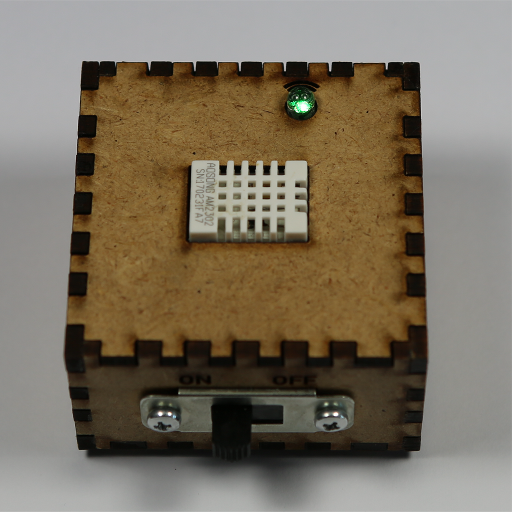
\includegraphics[width=1\linewidth]{bilder/chapter1/DHT22.png}
        \caption{}
        \label{fig:gull}
    \end{subfigure}
    \quad
    \begin{subfigure}[b]{0.3\textwidth}
        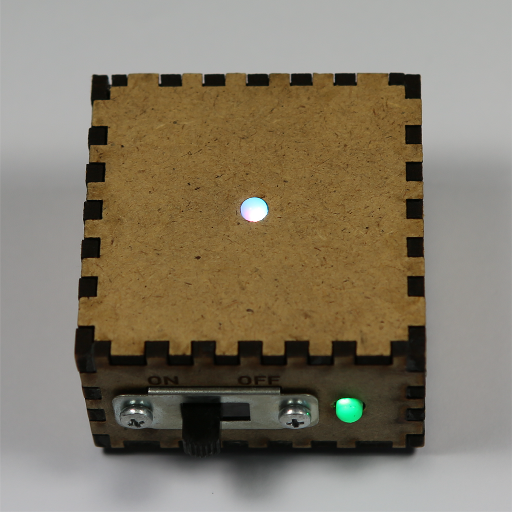
\includegraphics[width=1\linewidth]{bilder/chapter1/LED.png}
        \caption{}
        \label{fig:tiger}
    \end{subfigure}
    \quad
    \begin{subfigure}[b]{0.3\textwidth}
        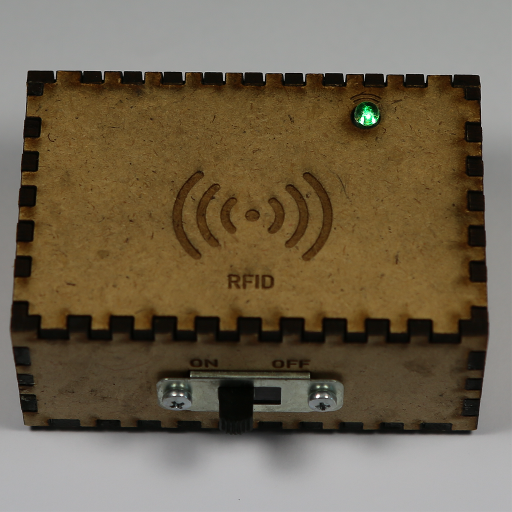
\includegraphics[width=1\linewidth]{bilder/chapter1/RFID.png}
        \caption{}
        \label{fig:mouse}
    \end{subfigure}
    \caption{Typische \acp{cBlocks}. Hier bestehend aus drei unterschiedlichen Blöcken: Temperatur-Sensor (a),  LED-Aktor (b) und RFID-Sensor (c)}
    \label{fig:cblockfoto}
\end{figure}


Im Zuge dessen, wurde die Hardwareplattform \acp{cBlock} entwickelt. \acp{cBlock} ist ein \textit{open-source} Bausteinsystem zur Unterstützung von Designern beim \textit{Rapid-Prototyping}-Prozess von \ac{IoT} Produkten. Ein jeder Baustein abstrahiert verschiedenen Sensoren oder Aktoren und versucht dadurch, die Komplexität von hardwarenahen Entwicklungsaufgaben (beispielsweise Verdrahtung der Komponenten, Kommunikation zwischen Sensoren und Aktuatoren, Wählen von Protokollen) zu reduzieren. Das wichtigste Ziel von \acp{cBlock} ist allerdings nicht nur eine Aufwandsreduzierung auf Hardware-Ebene durchzuführen, sondern auch die Eintrittsbarriere für die Programmierung der Logik herunter zusetzen. Dadurch soll der technische Arbeitsaufwand von Designern so reduziert werden, dass sie sich darauf fokussieren können, neue \ac{IoT}-Erfahrungen zu erproben.

\section{Zielsetzung}\label{sec:1_zielsetzung}
Wie im vorherigen Kapitel besprochen, ist die \acp{cBlock}-Hardware dafür gedacht, die Entwicklung von \ac{IoT} Prototypen zu vereinfachen. Allerdings beschränkt sich diese Verbesserung der Usability ausschließlich auf den Hardware-Aspekt von \ac{IoT}. Deshalb besteht das \textbf{Ziel} dieser Arbeit darin, dem \textit{End-User} (d.h. dem Designer) bei der Erstellung von Programmlogik, welche die \ac{cBlock} steuern, zu unterstützen. Hierfür wird eine \ac{EUD}-Plattform konzipiert und evaluiert, welche auf die Anforderungen der Domäne des \ac{IoT} sowie den Anforderungen der Domänenexperten, gerecht wird. Dieses \ac{EUD}-Werkzeug, genannt \textit{flowws}, soll es Designern ermöglichen zusammen mit der \acp{cBlock}-Hardware, funktionale Prototypen zu gestalten.

Folgende \textbf{Forschungsfragen} sollen beantwortet werden:
\begin{itemize}
    \item \textbf{Bestehende Ansätze} \ac{EUD}-Werkzeuge sind in der wissenschaftlichen Literatur ein seit den 1980ern behandeltes Thema. Trotzdem hat sich noch keine breit angenommene Theorie etabliert. In der Praxis haben sich allerdings mehrere Paradigmen durchgesetzt. Um eine Entscheidung für flowws zu treffen werden folgende Fragen deshalb behandelt:
    \begin{itemize}
        \item Welche Ansätze für \ac{EUD}-Werkzeuge haben sich etabliert, besonders im Bereich der \ac{IoT}?
        \item Was sind die Vor- und Nachteile der Paradigmen?
    \end{itemize}
    \item \textbf{Anforderungen} Wie schon im vorangeschrittenen Kapitel beschrieben, ist das Projekt durch spezielle Rahmenbedingungen bzgl. Prozessen und Stakeholdern gekennzeichnet. Deshalb die Frage:
    \begin{itemize}
        \item Welche fundamentalen Probleme müssen \ac{EUD}-Werkzeuge in der \ac{IoT}-Domäne überwinden?
        \item Welche Anforderungen stellt die \ac{IoT} und die involvierten Stakeholder an ein \ac{EUD}-Werkzeug?
    \end{itemize}
    \item \textbf{Evaluation} Im Anschluss zur Anforderungserhebung und Erarbeitung eines Konzepts eines \ac{EUD}-Werkzeuges soll die Wirksamkeit der Entscheidungen diskutiert und folgende Frage beantwortet werden: 
    \begin{itemize}
        \item Was sind die Vor- und Nachteile des erarbeiteten Konzepts?
        \item Inwiefern lassen sich die Erkenntnisse auf zukünftige Projekte in diesem Themenbereich übertragen?
    \end{itemize}
\end{itemize}

\paragraph{Abgrenzung} Es ist nicht Ziel dieser Arbeit eine vollständige \ac{EUD} für einen Produktiveinsatz (bspw. in Form einer Turing-Vollständigen \ac{DSL}) zu konzipieren, sondern vielmehr geeignete Metaphern finden und \ac{UI}-Ansätze zu konzipieren und zu evaluieren, um einen besseren Einblick für zukünftige Projekte im Bereich des \ac{IoT}-Prototyping zu erhalten. Des Weiteren, grenzt sich diese Arbeit von hardware-technisch ähnlichen Systemen wie bspw. eBlocks (\cite{Phalke.2010}) ab, indem der Anwendungsfokus nicht auf Werkzeug zur Bildung im Bereich Software Engineering oder \ac{IoT} gelegt wird. Vielmehr handelt es sich bei flowws um ein Entwicklungswerkezug, welches aktiv zur Erprobung und Entwicklung von \ac{IoT}-Prototypen dienen soll.

\section{Aufbau der Arbeit}\label{sec:1_aufbau}
\begin{itemize}
    \item \textbf{Kapitel 1 Einleitung:} Eine Übersicht über das Thema und dem Kontext indem sie entstanden ist.
    \item \textbf{Kapitel 2 Grundlagen und State-of-the-Art:} In diesem Kapitel, werden die fundamentalen Wissensbausteine der \ac{IoT}- und \ac{EUD}-Domäne diskutiert. Zusätzlich werden bestehende \acp{EUD}-Systeme mit vergleichbarem Fokus diskutiert.
    \item \textbf{Kapitel 3 Anforderungen:} In diesem Abschnitt, werden Probleme von bestehenden \acp{EUD}-Systemen und die Stakeholder anhand einer Persona analysiert. Daraus abgeleitet, entstehen Vision und Ziele für das \ac{EUD}-Werkzeug, welche wiederum in Szenarios und Anforderungen transformiert werden.
    \item \textbf{Kapitel 4 Konzeption:} Das \ac{EUD}-Werkzeug flowws wird in diesem Kapitel konzipiert und die getroffen Designentscheidungen werden rationalisiert.
    \item \textbf{Kapitel 5 Evaluation:} Das Konzeptmodell von flowws wird durch Nutzertests auf seine Verständlichkeit überprüft.
    \item \textbf{Kapitel 6 Diskussion:} Zum Schluss werden die erarbeiteten Ergebnisse zusammengefasst, bewertet und ein Ausblick für zukünftige Arbeiten gegeben.
\end{itemize} % Externe Datei einbinden
\chapter{Grundlagen und State-of-the-Art}\ref{GrundlagenSOTA}
Das Thema dieser Thesis befindet sich auf dem Schnittpunkt zweier Teilgebiete: \ac{IoT} und \ac{EUD}. Die Anwendungsdomäne ist ausschlaggebend für das Konzept eines \ac{EUD}-Werkzeugs [Quelle]. Deshalb werden werden in den folgenden Unterkapiteln die literarische Grundlage, bzgl. \ac{IoT} gelegt. Des Weiteren wird sich mit der Thematik des \acp{EUD} selbst, sowie dessen State-of-the-Art-Ansätze beschäftigt.


\section{Internet of Things}
\subsection{Vergangenheit, Gegenwart, Zukunft}
\begin{quote}
''\textit{The most profound technologies are those that disappear}'' \\-- Mark Weiser, Chief Technologist at Xerox PARC
\end{quote}

1991 schrieb M.Weiser in seinem einflussreichen Artikel \cite{weiser1991computer}, in dem er eine Zukunft beschrieb, in welcher der Computer komplett mit seiner Umgebung verschmilzt und somit unsichtbar für den Endnutzer wird. Dieses theoretische Paradigma wurde von ihm \ac{Ubicomp} -- die Allgegenwärtigkeit von Informationsverarbeitung -- getauft. Dieser Ansatz begründete sich auf den Erfolgen der \ac{GUI} als Interaktionsmodel über die, zu jener Zeit dominierende, textuelle Eingabe auf Konsolen-basis. Eine \ac{GUI} stellt im Optimalfall eine Metapher zur physischen Welt dar (bspw. Computer Desktop und reeller Schreibtisch). Nach \cite{weiser1991computer} wird es durch \ac{Ubicomp} möglich sein, diese Metaphern wieder zurückzuführen, d.h. die physische Welt wird durch die Verdrahtung mit seinen digitalen Repräsentanten wieder zusammengeführt. Das Ziel von \ac{Ubicomp} ist somit, die Einbettung des Computers in der physischen Welt, statt einer Manifestation der reellen Welt innerhalb des Computers (\cite{lyytinen2002ubiquitous}). 

Anfang der neunziger Jahre, war dieses Paradigma aufgrund fehlender Technologien nur schwer in die Realität umzusetzen. Kabellose Übertragung von Daten war weder standardisiert noch technisch weit genug fortgeschritten, unzureichende Energiespeicher und die fehlende Rechenkapazität von Computern waren nur einige Hindernisse, die zu diesem Zeitpunkt einer Verbreitung des \ac{Ubicomp} Paradigmas, außerhalb von wissenschaftlichen Experimenten im Weg stand \cite{lyytinen2002ubiquitous}.

Die Erfüllung zweier Regeln, haben sich für die Entwicklung der fehlenden Technologien als wichtig erwiesen: Komey's Law \cite{koomey2010law} und Moore's Law \cite{schaller1997moore}. Sie sagen voraus, dass alle 18 Monate sich der Preis pro Transistor halbiert und sich die Energieeffizienz gleichzeitig verdoppelt. Gut 30 Jahre nach der initialen Vision von \ac{Ubicomp} sind leistungsfähige Computer auf die Größe einer Streichholzschachtel geschrumpft, dauerhaft mit dem Internet verbunden und günstig. Durch diese stetige Verbesserung mobiler Hardware, das Durchsetzen von Kommunikationsprotokollen wie \textit{6LoWPAN} und die Motivation der Industrie, Prozesse immer weiter zu automatisieren (d.h. Industrie 4.0), hat sich das \acf{IoT} in seiner jetzigen Form entwickelt.

Der Befriff \ac{IoT} wurde 2002 in \cite{ashton2009internet} mit dem Zitat:
\begin{quote}
    ''\textit{We need an internet for things, a standardized way for computers to understand the real world}''
\end{quote}
 geschaffen. Hierbei bezog sich \cite{ashton2009internet} auf die RFID-Technologie, welche es erlaubt reellen Objekten (engl. ''Things'') durch einen ID-Tag eine Identifikation und somit eine virtuelle Repräsentation zuzuweisen. RFID ist allerdings mehr als nur ein Barcode, denn es erlaubt Position und Status eines \textit{Things} in Echtzeit zu verfolgen \cite{atzori2010internet}. Dieses Erzeugen eines virtuellen Abbilds gilt als Schlüssel-Technologie für das \ac{IoT}. Seit 2002 haben sich die zugrunde liegenden Technologien stetig weiterentwickelt und somit die Vision erweitert. \ac{IoT} hat sich zu einem der brisantesten Paradigmen des 21. Jahrhunderts entwickelt. Schon jetzt, existieren laut \cite{gartnerIoT} über 6.4 Milliarden \textit{Things} bzw. \textit{Smart Objects}, welche miteinander kommunizieren. Der anhaltende Trend der Digitalisierung von Alltagsleben und Industrieprozessen durch \ac{IoT}, soll im Jahr 2020 die Anzahl von \textit{Smart Objects} auf über 21 Milliarden erhöhen. Zu diesem Zeitpunkt wird laut \cite{tan2010future} die Maschine-zu-Maschine (\textit{thing-to-thing}) Kommunikation, die der Mensch-zu-Mensch Kommunikation quantitativ übersteigen. Dieser Zuwachs an \textit{Things} und das einbinden neuer Technologien (bspw. Künstliche Intelligenz, siehe \cite{mehdi2017deeplearningIoT}) wird auch in Zukunft noch die Anforderungen und Visionen an \ac{IoT} formen \cite{Gubbi.2013}.
 
\subsection{Begriffsdefinition}
Das \acl{IoT} ist bestenfalls ein schwammig definierter Begriff. Es existiert keine breit angenommene Definition für \ac{IoT} \cite{atzori2010internet}. Dieses wird dadurch erschwert, dass durch die domänenübergreifende, organisatorische und technische Vielfalt innerhalb von \ac{IoT}-Systemen sowie die breite Anwendungsspektrum von \ac{IoT} verschiedene Visionen für das Paradigma entstanden sind. \cite{atzori2010internet} hat versucht diese Visionen in drei verschiedene Sichtweisen unterteilt: 

\paragraph{\textit{Things} orientiert} Hierbei handelt es sich um die originale Vision der Auto-ID labs bzw. die von \cite{sarma2000networked} vorgestellt wurde:

\begin{quote}
    ''\textit{we envision a world in which all electronic devices are networked and every object, whether it is physical or electronic, is electronically tagged with information pertinent to that object.}''
\end{quote}

Diese Vision von \ac{IoT} reflektiert die Anfänge des Begriffs, bei denen wenig Augenmerk auf Maschine-zu-Maschine Kommunikation gelegt wird. Vielmehr liegt der Fokus an dieser Stelle auf den \textit{Smart Objects}: Ihre Charakteristik (bspw. Identität, Verhalten, Intelligenz), Ausprägung (bspw. Sensor, Aktor, Transducer) und die hierbei genutzten Technologien (bspw. RFID, NFC, WISP).

\paragraph{Internet orientiert} In diesem Falle, wurde das Hauptaugenmerk der Vision auf die Kommunikation zwischen den einzelnen \textit{Smart Objects} gelegt. Aus dieser Sichtweise, definiert sich \ac{IoT} über die Standardisierung der Kommunikation, die Architektur und Orchestrierung von \ac{IoT}-Ökosystemen und die dafür notwendige Technologien (bspw. 6LoWPAN, MQTT). Das \ac{ITU} definiert seine Vision von \ac{IoT} in \cite{itut2012}, wie folgt: 

\begin{quote}
''\textit{a global infrastructure for the Information Society, enabling advanced services by interconnecting (physical and virtual) things based on, existing and evolving, interoperable information and communication technologies}''
\end{quote}

Diese Internet-zentrische Vision entspringt aus der Notwendigkeit, dass die schiere Masse an \textit{Things} neue Anforderungen an die Technik stellt (bspw. Erweiterung des Adressraums duch IPv6). 

\paragraph{Semantik orientiert} Die auf Wissen basierende Visionen zählen zu den neueren Perspektiven der \ac{IoT}. Hierbei ist der Schwerpunkt nicht die Kommunikation und die beteiligten \textit{Smart Objects} sondern die Eigenschaften der ausgetauschten Daten, wie sie ausgetauscht, aufbereitet und gespeichert werden. In \cite{Kotis2012} und \cite{Singh2014} wird diese Vision beschrieben. Hierbei werden neue Herausforderungen wie die Interoperabilität von \textit{Smart Objects}, Sicherheit, Privatsphäre \cite{weber2010internet} und die Dringlichkeit neuer Speichertechnologien in den Vordergrund gestellt.

\begin{figure}
    \centering
    \begin{tikzpicture}[every path/.append style={fill opacity=0.75},]
      \begin{scope}[blend group = lighten]
        \fill[red!30!white]   ( 90:1.2) circle (2);
        \fill[green!30!white] (210:1.2) circle (2);
        \fill[blue!30!white]  (330:1.2) circle (2);
      \end{scope}
      \node at ( 90:2)    {Semantik};
      \node at ( 210:2)   {Internet};
      \node at ( 330:2)   {Things};
      \node [font=\Large] {\ac{IoT}};
    \end{tikzpicture}
    \caption{Das momentane Verständnis des \ac{IoT}-Begriffs stützt sich auf eine semantische, physische und kommunikative Sichtweise der Probleme. Darstellung angelehnt an \cite{atzori2010internet}}
    \label{fig:visions}
\end{figure}


Wie vorgestellten Visionen (Abbildung \ref{fig:visions}) reflektieren die Bestandteile eines \ac{IoT}-Systems aber auch die geschichtliche Herkunft des Paradigmas: von der Schaffung identifizierbarer \textit{Things} über der Kommunikation zwischen \textit{Smart Objects} zu der Semantik ausgetauschter Information. Es ist auch ersichtlich, dass cyx Verständnis von \ac{IoT} noch nicht komplett ausgereift ist (\cite{atzori2010internet}). Deshalb ist es schwierig, eine allgemeingültige, auch in Zukunft treffende Definition, von \ac{IoT} zu formulieren. Mit dem Hinblick zu potentiellen Folgeparadigmen, wie das Internet of Everything (\cite{Snyder2017}), ist es ohnehin fraglich ob \ac{IoT} nur eine Zwischenstadium darstellt. Nichts desto trotz, wird für diese Thesis die in \cite{Misra2017} zu findende Definition verwendet: 
\begin{quote}
   ''\textit{The \ac{IoT}, a global network infrastructure, links uniquely identified physical and virtual objects, things and devices through the exploitation of data capture (sensing), communication and actuation capabilities. The underlying infrastructure of virtually represented ''things'' in an Internet-like structure includes existing and evolving Internet and network developments. Emerging services and applications will be characterised by a high degree of autonomous data capture, event transfer, network connectivity and interoperability.}''
\end{quote}

Diese Definition vereint die vorherigen Visionen (\textit{Smart Objects}/\textit{Things}, Internet und Semantik) in einem treffenden Paragraph, ohne besonderes Augenmerk auf gewählten Technologien zu legen. Es wird ersichtlich, welche Objekte beteiligt sind, dass sie in einer Struktur verbunden werden müssen und autonom Daten austauschen müssen, um einen Mehrwert in Form von \textit{Services} darstellen zu können. 


\subsection{Charakterisierung von IoT}\label{subsec:characIot}
Wichtiger als die Definition von \ac{IoT} ist für diese Arbeit die Charakterisierung von \ac{IoT}. Hierbei werden die einzelnen Bestandteile eines \ac{IoT}-Systems definiert und ihr Zusammenspiel beschreiben. Wie der Name von \acl{IoT} vermuten lässt, besteht es aus zwei Bestandteilen \textbf{Internet} und \textbf{Things}.

\subsection{Things}
\textit{Things} ist der Oberbegriff für die physischen Objekte innerhalb einer \ac{IoT} Landschaft, die mit Umwelt und User interagieren. In diesem Zusammenhang sind zwei Begriffe von Bedeutung: \textbf{\ac{WSAN}} und \textbf{Smart Objects/connected Objects}.

\subsubsection{Smart Objects}
\textit{Smart Objects} stellen komplexe Interaktionsobjekte dar und sind auf der Komponentenebene die physikalischen Repräsentanten des Gesamtsystems. Ein \textit{Smart Object} kann aus ein oder mehreren Sensoren und Aktoren bestehen. \cite{Kortuem2010Smart} definiert \textit{Smart Objects} als ein dezentralisiertes System von lose gekoppelten, autonomen, physikalisch sowie digitalen identifizierbaren Objekten mit der Möglichkeit ihre Umgebung durch Sensoren wahrzunehmen, diese Daten zu verarbeiten und über ein geteiltes Medium zu kommunizieren. \cite{mattern2010internet} beschreibt zusätzlich den Begriff der \textit{Effektorik} hierdurch wird es \textit{Smart Objects} möglich, durch Aktoren digitale Signale in  physikalische Signale (bspw. Bewegung durch Motoren oder visuelle Reize durch LEDs) zu transformieren. \cite{Kortuem2010Smart} beschreibt die grundsätzliche Charakteristiken von \textit{Smart Objects} wie folgt:
\begin{itemize}
    \item \textbf{Bewusstsein} Ein \textit{Smart Object} ist in der Lage seine Umgebung und/oder das Verhalten des Users zu wahrzunehmen und entsprechen der einprogrammierten Intelligenz darauf zu reagieren. \textit{Smartness} ist allerdings ein sehr dehnbarer Begriff. Hierbei ist nicht zwingend künstliche Intelligenz gemeint, sondern schlichtweg das autonome Analysieren, Verarbeiten und Speichern von Daten. Für folgende Komponenten können \textit{Smart Objects} ein Bewusstseins besitzen:
    \begin{itemize}
        \item \textbf{Aktivitäten/Events} Events bzw. Aktivitäten werden von \textit{Smart Objects} erfasst. Diese Ströme von Daten (bspw. Temperatur) oder Events (bspw. Taster wird betätigt) treten asynchron und in aperiodischen Zeitspannen auf. Ziel von \textit{Smart Objects} ist es solcher spontan entstehender Daten zu erfassen und weiter zu verarbeiten.
        \item \textbf{Prozesse} Komplexere \textit{Smart Objects} können ein Bewusstsein für Abläufe von Prozesse besitzen die von umgebungsbedingter (bspw. Tag-Nacht-Zyklus) oder organisatorischer (bspw. Geschäftsprozess) Natur sind. Einem \textit{Smart Device} ist es möglich Soll-Ist Vergleiche zwischen den Abläufen zu erstellen und danach zu handeln.
    \end{itemize}
    \item \textbf{Darstellung} Hierbei wird die Abstraktion der Logik, des \textit{Smart Objects} definiert. Unterschiedliche \textit{Smart Objects} können abhängig von ihrer Anwendung und der Komplexität ihrer Interaktion unterschiedlich gut geeignete für Programmiermodelle besitzen.
    \begin{itemize}
        \item \textbf{Aggregierende Funktionen} \textit{Events} und Datenströme können von \textit{Smart Objects} zusammengefasst, verfeinert und simplifiziert werden. Die resultierenden Daten können dann von Teilkomponenten des Gesamtsystems weiterverarbeitet werden. In solchen Fällen ist die Darstellung beschränkt auf die Darstellung der Logik mathematische Funktionen.
        \item \textbf{Regeln} Dies ist ein weiterführendes Konzept der aggregierenden Funktionen. Hierbei werden \textit{Events} und \textit{Streams} nicht nur zusammengefasst, sondern auch mit einer Regel (''Wenn \textit{Event x} dann \textit{Aktion y}'') gesteuert. Erfüllung bzw. Nichterfüllung der Regeln können verschiedene Aktion innerhalb und außerhalb des \textit{Smart Objects} hervorrufen.
        \item \textbf{Workflow} Das Ziel dieses Programmierparadigmas ist die sequentielle Abarbeitung von Arbeitsschritten zu modellieren. Dies ermöglicht es dem \textit{Smart Object} Prozess-Kontext nahe Interaktionen abzubilden.
    \end{itemize}
    \item \textbf{Interaktion} Das \textit{Smart Object} wird durch eine Reihe von Interaktionen charackterisiert, die es mit dem Nutzer und seiner Umgebung, durchführen kann. Die Arten von Interaktionen sind wie folgt definiert:
    \begin{itemize}
        \item \textbf{Keine Interaktion} Laut [\cite{mattern2010internet}], müssen \textit{Smart Objects} nicht zwingend Interaktionen auf einer physischen Ebene besitzen. Auch passive Aggregation von Daten (bspw. Positionsverfolgung von Geräten) kann einen Mehrwert für den User oder Organisationen bringen.
        \item \textbf{Kontext-Interaktion} Durch das Akkumulieren von \textit{Streams} und Events können \textit{Smart Objects} Interaktionen mit dem User auslösen bzw. audio/visuelles/haptisches Feedback geben. 
        \item \textbf{Prozess-Interaktion} Als komplexeste Interaktion wird die Interaktion im Prozess-Kontext erachtet. Hierbei ist es dem Objekt möglich, abhängig des Prozess-Schrittes in dem es sich befindet, dem User und der Umgebung zu interagieren.
    \end{itemize}
\end{itemize}
Um \textit{Smart Objects} noch besser klassifizieren zu können, hat \cite{lopez2011taxonomy} das Modell ''I-S-A-D-N'' entworfen, welches es ermöglicht die \textit{Smart Objects} anhand ihrer Fähigkeiten zu Klassifizieren. Jeder Buchstabe in ''I-S-A-D-N'' steht für eine Fähigkeit und kann beliebig kombiniert werden (\ref{tab:isadnKennz}). 
\begin{table}[H]
\centering
\label{tab:isadnKennz}
\begin{tabularx}{\textwidth}{llX}
\hline
\rowcolor[HTML]{EFEFEF} 
Kennz. & Bedeutung & Beschreibung \\ \hline
I      & Identität      & Das Objekt besitzt eine eindeutige Identität und die Möglichkeit Daten zu speichern. \\ \hline
S      & Sensorik       & Hierbei besitzt das Smart Device die Fähigkeit Daten aus seiner Umwelt zu erfassen. \\ \hline
A      & Aktorik        & Durch den Besitz von Aktoren oder den Zugang zu externen Aktoren kann das Device seine Umwelt manipulieren. \\ \hline
D      & Determinierend & Das Objekt besitzt die Möglichkeit selbständig, auf Basis eines vorprogrammierten Verhaltens und anhand von gesammelten Daten, Entscheidungen treffen. Diese Entscheidungen können zu neuen physischen und digitalen Signalen führen. \\ \hline
N      & Netzwerkend   & Durch Einbindung in ein Netzwerk kann ein Objekt, bidirektional sich mit anderen Smart Objects über kabellose und kabelgebundene Kommunikationskanäle austauschen. \\ \hline                                                        
\end{tabularx}
\caption{Aspekte des ''I-S-A-D-N'' Intelligenz-Klassifikationsmodells für \textit{Smart Objects} nach \cite{lopez2011taxonomy} }
\end{table}

Je nach Komplexität des \textit{Smart Objects} können verschiedene Kombinationen von Kennzeichen entstehen. Ein ISN-Objekt is ein \textit{Smart Object}, welches Identifizierbar ist, seine Umgebung bemisst und diese Daten speichert bzw. über das Netzwerk mit anderen Objekten kommuniziert. Als Einschränkung hierbei nennt \cite{lopez2011taxonomy}, dass ein \textit{Smart Device} mindestens IN-Fähigkeiten besitzt, also mindestens eine Identität besitzt und diese kommunizieren kann.

\subsubsection{\acl{WSAN}}\label{subsubsec:wsan}
\begin{figure}[h]
    \centering
    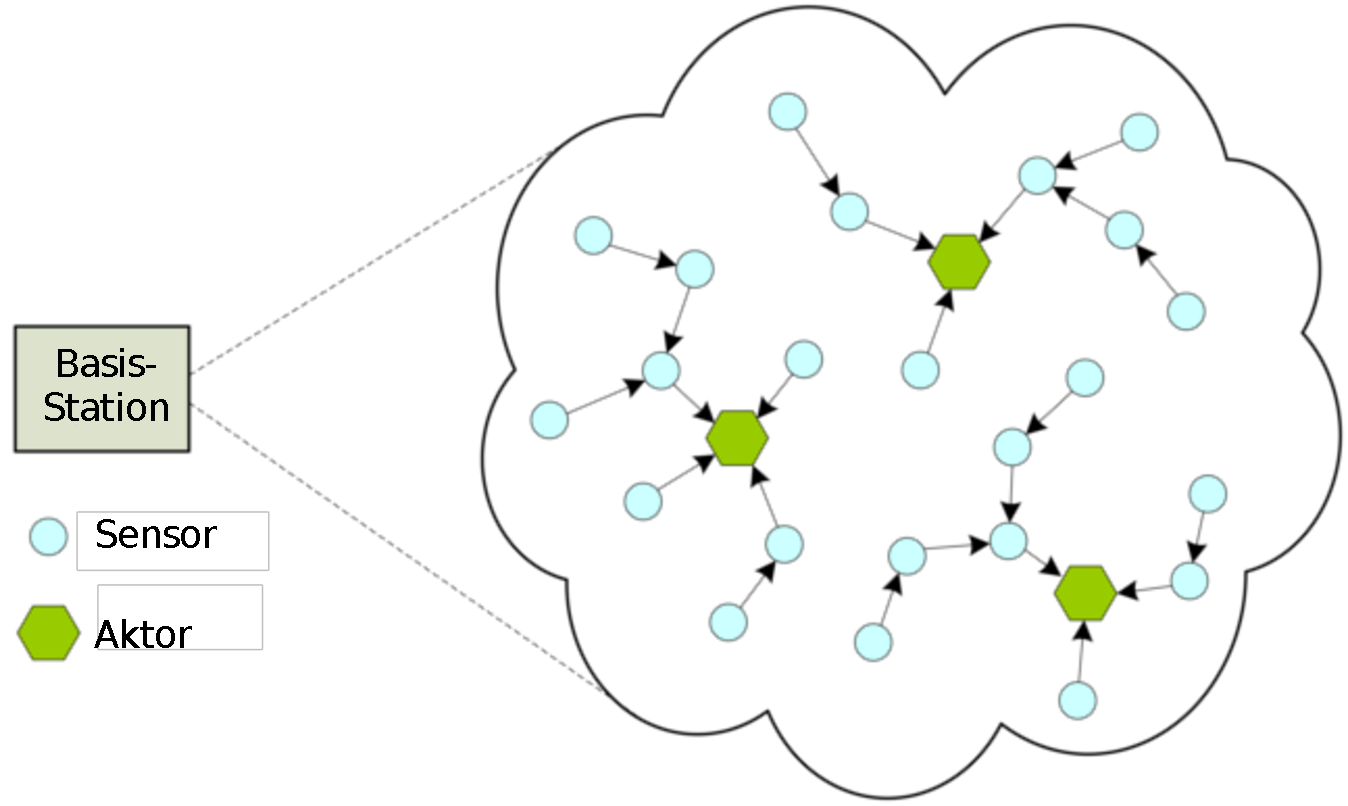
\includegraphics[width=0.7\textwidth]{bilder/chapter2/wsan.pdf}
    \caption{Ein typisches \ac{WSAN} nach \cite{feng2008wsan}. Zu sehen sind Aktoren und Sensorknoten die in einem Netzwerk miteinander kommunizieren, welches von einer Basisstation aufgespannt wird}
    \label{fig:WSAN}
\end{figure}
\ac{WSAN} ist ein weiterer historisch und technisch wichtiger Baustein des \ac{IoT} Ökosystems. Es beschreibt die Architektur und Module, welche durch kabellose Kommunikation sich in einem Netzwerk organisieren (\cite{ferrara2013smart}). Die Abgrenzung von \ac{WSAN} zu \textit{Smart Objects} liegt darin, dass \ac{WSAN} sich weniger auf explizite Interaktionen mit dem User fokussieren, sondern sich vielmehr mit dem Erfassen und Erzeugen von Umgebungssignalen (bspw. Feuchtigkeit, Helligkeit, etc.) beschäftigen (\cite{Madakam2015litRev}). \ac{WSAN}-Forschung ist \ac{IoT} vorangegangen. Der wissenschaftliche Fokus von \ac{WSAN}-Forschung liegt in der Reduktion von Energieverbrauch, physikalischer Größe, Vergrößerung von Senderadius und Verbesserung der Sensorik und Aktorik. Von dieser Entwicklung profitierte auch \ac{IoT} (\cite{lopez2011taxonomy}).

\ac{WSAN} bestehen von einer Top-Level-Ansicht (siehe Abbildung \ref{fig:WSAN}) aus zwei Konstrukten: \textbf{Motes} (dt. ''Staubkorn'') und \textbf{Sinks} (dt. ''Senke''). Diese Komponenten werden als \textbf{Nodes} (dt. ''Knoten'') und stellen die Knotenpunkte eines \acp{WSAN} dar. Sie bestehen aus autarken Embedded-Computern, welche entweder als Sensoren oder Aktoren. Nodes mit Sensoren werden als Mote bezeichnet (\cite{salarian2012coordination}) und erfassen die physischen Signale der Umgebung. Sinks bezeichnen hierarchisch übergeordnete Knotenpunkte innerhalb eines \ac{WSAN}. Sinks sind Aktoren, die durch das Bündeln vom Datenverkehr der Motes, physikalische Signale erzeugen mit denen sie Einfluss auf die reale Umwelt nehmen.

Bei \ac{WSAN} als auch bei \textit{Smart Objects} kristallisieren sich als fundamentale Bausteine \textbf{Sensoren} und \textbf{Aktoren} heraus. Aufgrund ihrer tragenden Rolle für \ac{IoT}, werden die Komponenten anhand eines Domänen-Modells (siehe Abbildung \ref{fig:ActuatorSensorDomainmodel}) erklärt.
\begin{figure}[h]
    \centering
    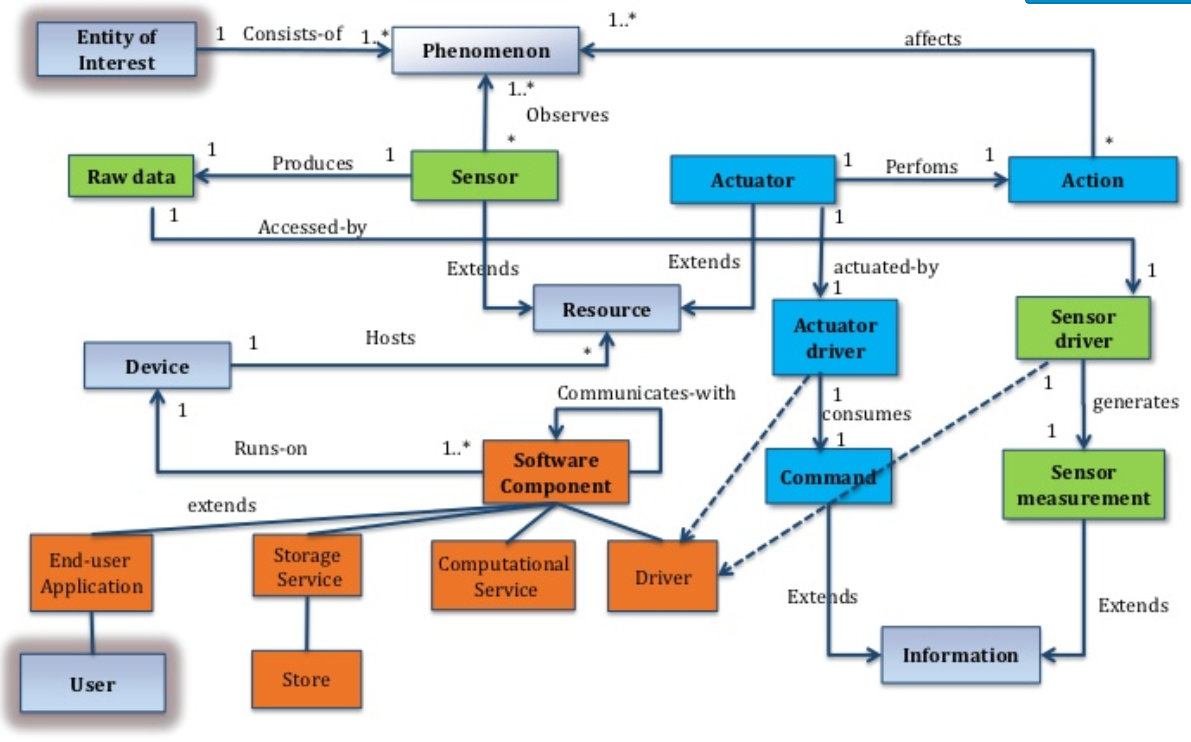
\includegraphics[width=0.75\textwidth]{bilder/chapter2/domainmodel.png}
    \caption{Domänenmodell für Aktoren und Sensoren innerhalb eins \ac{WSAN}}
    \label{fig:ActuatorSensorDomainmodel}
\end{figure}

\paragraph{Sensoren} sind ein essentieller Part vieler moderner Maschinen. Sie sind analog mit den fünf Sinnen des Menschen insofern, dass sie Computern erlauben, ihre Umgebung wahrzunehmen. Diese Wahrnehmung geschieht durch das Transformieren von (elektro-)magnetischer, akustischer und chemischer Signale in digitale und analoge Impulse. Diese Transformation von physikalischen Phänomenen in elektrische Signale macht jeden Sensor essentiell zu einem Transducer (engl. ''Wandler''). 
\begin{figure}[h]
    \centering
    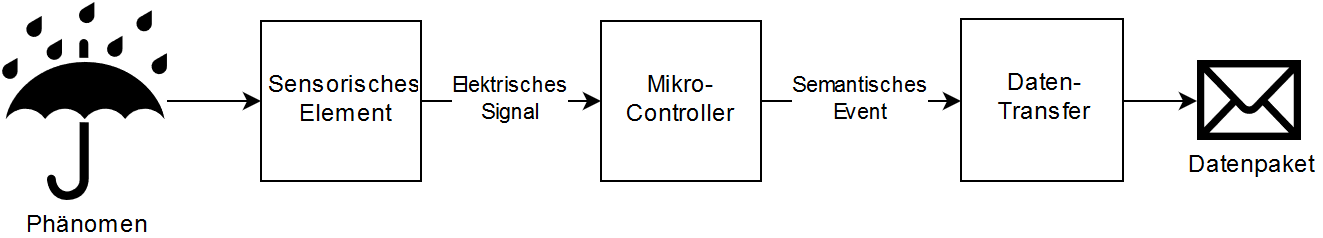
\includegraphics[width=0.75\textwidth]{bilder/chapter2/smartsensor.png}
    \caption{Als Smart-Sensor wird ein Sensor bezeichnet, der zusätzlich zu seinen Fähigkeiten als Transducer (physikal-zu-digital Wandler) diese Signale in Events bzw. Datenpakete mit semantischer Bedeutung transformieren kann (\cite{rayes2017internet}).}
    \label{fig:Smartsensor}
\end{figure}
Messungen, die ein Sensor nimmt, sind unbearbeitet (siehe \ref{fig:ActuatorSensorDomainmodel}) und reflektieren die zugrunde liegenden Technik des Sensors (bspw. Schwankungen im Widerstand). Dieser ''rohe'' \textit{Output} ist nur schwer interpretierbar für Menschen. Erst eine Zuweisung von unbearbeitetem Output auf vorgegebene Werte gibt dem Output eine semantische Bedeutung. Dieser Vorgang ist in Abbildung \ref{fig:Smartsensor} illustriert. \cite{rayes2017internet} spricht hierbei von einem Smart-Sensor, da er eine programmierte Intelligenz besitzt, welche ein physikalischen Phänomena in ein semantisches Datenpaket umwandeln kann.

\begin{table}[H]
\centering
    \resizebox{\textwidth}{!}{
    \begin{tabular}{lllll}
    \hline
    \rowcolor[HTML]{EFEFEF} 
    Physikalisches Signal & Beispiel          & Output                  & Output-Format  & Einheit \\ \hline
    (Elektro)Magnetisch   & Erdmagnetfeld     & Himmelsrichtung         & $[0;360] $     & Grad    \\ \hline
    Chemisch              & $CO_{2}$-Sensor  & $CO_{2}$-Konzentration & $[0;100]$      & PPM     \\ \hline
    Akustisch             & Ultraschallsensor & Distanz                 & $[10;120]$     & cm      \\ \hline
    Position              & GPS               & Koordinaten             & $([-90;+90],[-180; 180])$  & (Längengr, Breitengr) \\  \hline
    Photoelektrisch       & Bewegungsmelder   & Bewegung                & ${True,False}$ & Boolean \\  \hline
    \end{tabular}
    }
\caption{Sensortypen und beispielhafte Vertreter. Obwohl sämtliche Sensoren analoge bzw. digitale Daten schicken, Sensoren können stark unterschiedliche Outputs besitzen. Tabelle angelehnt an \cite{lopez2011taxonomy}}
\label{tab:sensorbsps}
\end{table}

In Tabelle \ref{tab:sensorbsps} gibt es eine Aufstellung von Sensor-Typen, sowie Beispiele aus der jeweiligen Klasse. Wichtig ist hierbei anzumerken, dass es für fast jegliche Art von zu erfassenden Daten es mehrere alternative Sensortechnologien existieren. Ausschlaggebend können hierbei Kriterien wie die Kosten, Reaktionszeiten, Genauigkeit und Formfaktors des Sensors sein. Auch die Umgebung selbst kann ausschlaggebend für den Sensor-Typ sein.

\paragraph{Aktoren} stellen Wandler oder ''\textit{Transducer}'' dar, welche digitale Signale in physikalische Phänomene umwandeln. Diese Aktionen ermöglichen es, einem \ac{IoT}-System seine Umwelt zu manipulieren und auf Interaktionen mit dem Usern zu reagieren. 

\begin{table}[H]
\centering
\resizebox{\textwidth}{!}{
    \begin{tabular}{lllll}
    \hline
    \rowcolor[HTML]{EFEFEF} 
    Physikalisches Aktion & Beispiel           & Output-Typ  & Wertebereich    & Einheit         \\ \hline
    Visuell               & RGB LED            & Lichtimpuls & $[0;360]$       & RGB-Wert        \\ \hline
    Bewegung              & elektrischer Motor & Rotation    & $[-100;100]$ & Geschwindigkeit    \\ \hline
    Akustisch             & Lautsprecher       & Geräusch    & $[10;120]$      & Dezibel         \\ \hline
    \end{tabular}}
\caption{Typen von Aktoren}
\label{tab:typesOfActutors}
\end{table}

Die Definition von Aktor ist unterschiedlich, während eine Anzahl von Quellen auf die traditionelle Definition von Aktor (''Umwandeln von elektrischem Signal in mechanische Bewegung'') bevorzugen, wird im \ac{IoT}-Kontext auch oft Transducer, welche Visuelle/Elektromagnetische Phänomene erzeugen Aktoren bezeichnet (\cite{Dunko2006reference}). Da ein Relais, welches mechanisch eine Ampel steuert (\cite{salarian2012coordination}), als Aktor im traditionellen Sinn gilt, ist auch schlüssig eine Knoten, welcher digital eine LED ansteuert, auch als Aktor zu bezeichnen. Aus diesem Grund wird die \ac{IoT}-zentrische Verständnis von Aktoren für den Rest der Thesis verwendet. In Tabelle \ref{tab:typesOfActutors} ist eine Liste mit Beispielen von Aktor-Typen. 

\subsection{Internet}
Kommunikation, Orchestrierung und Interoperabilität zwischen \textit{Things} stellt die zweite Säule des \acp{IoT} dar. Ähnlich wie bei der Definition von \textit{Things}, existiert auch hier keine breit angenommene Begriffserklärung und verwendete Technologien. Die Kommunikation zwischen \textit{Things} ist facettenreich und und kann von verschiedenen Blickwinkeln betrachtet werden: Der verwendeten Technologien, der Organisationsstruktur oder der Semantik (bspw. Interoperabilitäts-Protokolle). Da sich diese Arbeit u.\,a. damit auseinandersetzt, treffende Metaphern für die Domäne der \ac{IoT} zu finden, ist organisatorische bzw. architekturelle Aspekt, der Interessanteste.
\begin{figure}[h]
    \centering
    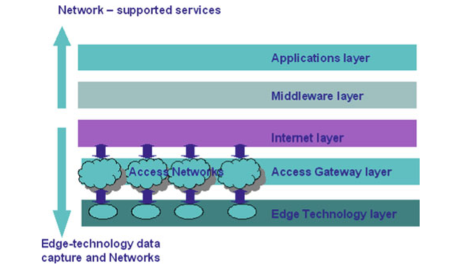
\includegraphics[width=0.75\textwidth]{bilder/chapter2/iotlayers.png}
    \caption{Schichtenmodell von einer typischen \ac{IoT} Infrastruktur nach \cite{bandyopadhyay2011internet}}
    \label{fig:iotlayer}
\end{figure}
Eine abstrahierte Version der \ac{IoT}-Architektur, welche wenig Wert auf verwendete Technologien legt, ist in Abbildung \ref{fig:iotlayer} zu sehen. Laut \cite{bandyopadhyay2011internet} besteht eine solche Architektur aus sechs Schichten. Die unteren drei Schichten setzen sich direkt mit dem Erheben und dem Transport von Daten auseinandersetzen. Diese Schichten befinden sich nah an der Grenze zur physikalischen Welt und werden deshalb als Edge-Layer bezeichnet. Die oberen Schichten beschäftigen sich mit der Transformation und Filterung der Daten, in einer Form, dass sie von Endnutzer-Applikationen verwendet werden können.  

\paragraph{Edge-Schicht} wurde in den vorherigen Kapitel schon beschrieben. Es handelt sich hierbei um die konkreten Physikalischen Ressourcen: Sensoren und Aktoren bzw. \textit{Smart Objects}. Alle Objekte auf dieser Ebene sind eindeutig Identifizierbar (bspw. via RFID), besitzen die Möglichkeit physikalische Signale in elektrische umzuwandeln (bzw. umgekehrt) und per Kommunikationsmedium (bspw. WiFi oder Bluetooth) mit der darüberliegenden Schicht zu teilen.

\paragraph{Access-Gateway-Schicht} verbindet die Objekte der Edge-Schicht, bündelt die im \ac{IoT}-System erzeugten Daten und verschickt diese an die weiterverarbeitenden Schnittstellen. Auch das \textit{Monitoring} von Objekten und Datensicherheit spielt auf dieser Ebene eine tragende Rolle. 

\paragraph{Internet-Schicht} symbolisiert das unterliegende Kommunikationsmedium, das Internet. Daten, die sich an der  Gateway-Schichte sammeln, werden über das Internet versendet. Diese Schicht beherbergt den Transport Layer des OSI-Modells inklusive UDP/TCP/IP-Stack und HTTP.

\paragraph{Middleware-Schicht} ist die erste reine Software-Schicht. Sie bildet das softwareseitige Herzstück des \ac{IoT}-Stacks und befasst sich damit, den bidirektionalen Austausch von Daten zu ermöglichen und den softwareseitigen Zugriff auf das \ac{IoT} System zu verwalten. Hierfür hat sich das \ac{SOA} Paradigma in der Vergangenheit für wegweisend erwiesen (\cite{laliwala2008event}).
\begin{figure}[h]
    \centering
    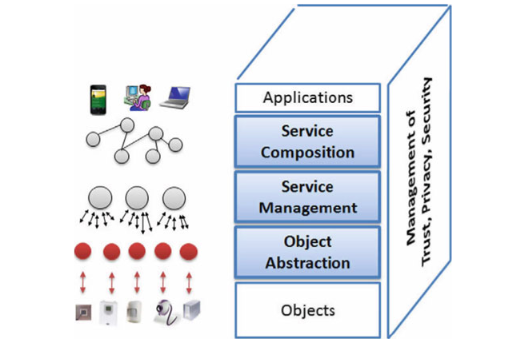
\includegraphics[width=0.75\textwidth]{bilder/chapter2/iotsoa.png}
    \caption{IoT Middleware-Schicht als \ac{SOA} nach \cite{bandyopadhyay2011internet}}
    \label{fig:iotsoa}
\end{figure}
Wie in Abbildung \ref{fig:iotsoa} zu sehen ist, abstrahiert die Middleware heterogene \textit{Smart Objects} bzw. Nodes in adressierbare, eindeutig identifizierbare, virtuelle Ressourcen (\textit{Object Abstraction}). Die Middleware kapselt einzelne oder mehrere Ressourcen zu Services mit wohl definierten Schnittstellen zusammen um die Verwaltung und Nutzbarkeit der Objekte zu verbessern (\textit{Service Management}). Zu guter Letzt lassen sich einzelne Services zu Workflows, welche eine Businesslogik abbilden kompositionieren (\textit{Service Composition}). Durch dieses \ac{SOA}-Model erlaubt es die Middleware viele heterogene Ressourcen miteinander zu vereinigen und sie Applikationslogik bereitzustellen. 

Die \textbf{Kommunikation} zwischen den (virtuellen) Ressourcen bzw. den Services wird als aperiodisch, pallel und Event-basiert charakterisiert (\cite{serpanos2018iot}, \cite{laliwala2008event}, \cite{lan2014event}). Laut \cite{serpanos2018iot} wird die Signalverarbeitung in traditionell geschlossenen System in periodischen Zyklen ausgewertet. Dies ist in \ac{IoT}-Systemen aufgrund räumlicher Verteilung von Nodes und der gestiegene Energiebedarf durch kabellose Datenübertragung nicht praktikabel. Aus diesen Gründen, muss davon ausgegangen werden, dass Nodes ihre Daten in \textbf{aperiodischen} Zyklen zusenden. Des Weiteren wird durch seine verteilte Kommunikation innerhalb eines \ac{IoT}-Systems als parallel und asynchron charakterisiert. Hierbei stellen \textit{Events} laut \cite{serpanos2018iot} einen zentralen Baustein dar. Events sind Nachrichten (engl. ''\textit{Messages}''), die von Nodes erzeugt und konsumiert werden können. Events werden durch ein \textit{key-value pair} oder aufgrund ihrer Lebenszeit und temporalen Verarbeitung als \textit{time-value pair} beschrieben werden. Dieses key-value pair wird laut [\cite{serpanos2018iot}] durch ein fünffach Tupel beschrieben:
\begin{equation}
    \left \langle key, payload, sender, receiver, timestamp \right \rangle
\end{equation}
Diese Events werden zwischen den Nodes, (virtuelle) Sensoren und (virtuellen) Aktoren über definierte Kommunikationskanäle, sogenannte \textit{Links}, versendet. Ankommende Events werden von den Nodes reaktiv verarbeitet.

\subsection{Zusammenfassung}
In diesem Kapitel wurden die grundlegenden Züge von \ac{IoT} charakterisiert und definiert, die für diese Arbeit relevant sind. Der \ac{IoT}-Begriff umschließt die Kommunikation zwischen verteilten, digital identifizierbaren Objekten. Diese Objekte (\textit{Smart Objects}) unterschiedlicher Komplexität, erreichen es durch Datensammlung, Datenverarbeitung und physikalische Manipulation ihre Umwelt wahrnehmen bzw. in (Geschäfts-)Prozesse einzugreifen. Wahrnehmung und Manipulation wird durch die Verwendung von \textbf{Sensoren} und \textbf{Aktoren} erreicht. In einem Netzwerk solcher Objekte (d.\,h. Nodes), geschieht Kommunikation über ein kabelloses geteiltes Medium (bspw. WiFi) und in weiter verteilten Systemen, über das Internet. Nodes kommunizieren mit Events parallel in aperiodischen Zyklen miteinander diese Events werden transformiert und Enden in Aktionen, wie das Speichern/Präsentieren von Daten oder Interaktionen mit der Umwelt und dem Endnutzer.

Ziel von \ac{IoT} ist es, durch die Verschmelzung digitaler und reeller Welt, reichhaltigere Benutzerinteraktionen zu ermöglichen.


%\section{Prototyping}
%What designers think
%\url{http://ldt.stanford.edu/~jsulzen/james-sulzen-portfolio/classes/ED229b/Syllabus/ED229B/www.stanford.edu/class/ed229b/fall00/readings/p300-gould.pdf}

%\subsection{Design Prozess}
%\begin{itemize}
%    \item Rational Process vs. Action Process
%    \item Design Thinking
%    \item Explorative Development
%\end{itemize}
%\subsection{Open-Design / Meta-Design}
%\url{https://www.cambridge.org/core/services/aop-cambridge-core/content/view/95F20761B4BB6466358E007AE51DE1ED/S2053470117000257a.pdf/opendesign_a_state_of_the_art_review.pdf}

\section{End-User Development}
\subsection{Begriffserklärung}
Im 21. Jahrhundert verwendet fast jeder Berufszweig computergestützte Systeme, um effizienteres Arbeiten zu ermöglichen. Es ist allerdings unmöglich jegliche Software genau auf den Use-Case zu zuschneiden, da die Kapazitäten an professionellen Software-Ingenieuren schlichtweg nicht ausreicht. Endnutzer sollen diese Lücke füllen. Endnutzer sind Software-Nutzer, die sich intensiv mit ihrer Anwendungsdomäne beschäftigen und dafür tagtäglich Software verwenden aber nur Laienhaft mit Computerprogrammierung vertraut sind. In 2005 wurde von \cite{Scaffidi2005eudnumbers} geschätzt, dass die Anzahl der Endnutzer auf über 90 Millionen (in den Vereinigten Staaten) im Jahr 2012 anwachsen wird. Der Grund hierfür ist einfach: die stetige Diversifikation von Geschäftsfeldern und Spezialisierung der Anwendungsfälle von Software steht einer geringen Anzahl ausgebildeter Software Ingenieure gegenüber. Endnutzer unterscheiden sich von Entwicklern, indem sie oftmals wenig Verständnis für Programmierung haben aber starkes Domänenwissen besitzen. Ihr Ziel ist es nicht allgemeingültige Softwareartefakte zu erstellen, sondern bestehende Software auf die individuellen Bedürfnisse zuschneiden.

Die Begrifflichkeit des \acf{EUD} selbst wuchs aus ursprünglich aus dem Thema des \ac{EUP} und \ac{EUC}. Unter dem Begriff \ac{EUP} wurde zu Beginn Programmier- und Scriptsprachen verstanden, welche von der unterliegenden Hardware abstrahierten und Nicht-Software-Ingenieuren erstmals erlaubte, eigene Programme zu entwickeln und bestehende Softwaresysteme zu erweitern. In den 1970er und 1980er wurde aus diesem  Paradigma \ac{EUC}, unter dem man Programmiersprachen der vierten Generation zusammenfasst (bspw. SQL). Diese Sprachen besitzen ein wesentlich höheres Abstraktionsniveau von der darunterliegenden Programmlogik als traditionelle Programmiersprachen. Sprachen wie SQL tauschen ihre Allgemeingültigkeit (bspw. ist SQL nicht turing-vollständig) gegen ein auf die Domäne zugeschnittenes Programmierparadigma. Je nach Literaturquelle wird \ac{EUP} als vorherige Evolutionsstufe von \ac{EUD} gesehen oder oftmals Synonym mit \ac{EUD} verwendet. \ac{EUD} sollte daher als eine Obermenge der Paradigmen angesehen werden, dies wird besonders offensichtlich wenn Nachfolgeparadigmen wie \ac{EUSE} das \ac{EUD} Modell um einen Softwareentwicklungszyklus erweitert (\cite{Ko2011EUSE}).

Die für \ac{EUD} am weitesten verbreitete Definition ist von \cite{Lieberman.2006} und lautet wie folgt:

\begin{quote}
    ''\textit{End-User Development can be defined as a set of methods, techniques, and tools that allow users of software systems, who are acting as non-professional software developers, at some point to create, modify or extend a software artifact.}''
\end{quote}

\ac{EUD} umschließt alle Prozesse, Werkzeuge und (Programmier-)Paradigmen, welche es End-Nutzern (bspw. Domänen-Experten, Studenten, Designer) abstrahiert von Low-Level Programmierkenntnissen Software zu erzeugen, zu warten und zu erweitern. Von \cite{ko2004six} wurden anhand einer Nutzerstudie sechs Barrieren ermittelt, welche dem Erfolg eines \ac{EUD}-Werkzeugs im Weg stehen kann:
\begin{itemize}
    \item \textbf{Design-Barriere}: ''\textit{Ich weiß nicht wie man das Problem definieren kann.}'' Tritt auf wenn ein Endnutzer grundsätzliche Probleme hat, das Problem in einer Form zu designen, in der es vom Computer verarbeitet werden kann.
    \item \textbf{Auswahls-Barriere}: ''\textit{Ich kann das Problem definieren aber weiß nicht, welches Werkzeug mir dabei behilflich ist.}'' Der Endnutzer weiß wie er das Problem definieren soll, nicht aber, welche konkreten Elemente des \ac{EUD}-Werkzeugs ihm dabei helfen es zu lösen.
    \item \textbf{Koordinations-Barriere}: ''\textit{Ich weiß, welche Werkzeuge ich benutzen muss aber nicht wie ich sie miteinander agieren lasse.}'' Der Endnutzer hat in diesem Fall Schwierigkeiten, die einzelnen Komponenten des \ac{EUD}-Werkzeugs miteinander zu kombinieren um das Problem zu lösen. 
    \item \textbf{Verwendungs-Barriere}: ''\textit{Ich weiß, welches Werkzeug ich benutzen muss aber nicht wie es funktioniert.}'' Das \ac{EUD}-Werkzeug oder eine Teilkomponente ist nicht explizit in der Funktion, die es bereitstellt und erlaubt dem Endnutzer Fehler zu begehen. 
    \item \textbf{Verständnis-Barriere}: ''\textit{Das Werkzeug hat sich nicht so verhalten, wie es erwartet hatte.}'' Hierbei herscht eine kognitive Diskrepanz zwischen dem Verhalten dass der Endnutzer von einer \ac{EUD}-Notation erwartet, und wie sie sich tatsächlich verhält.
    \item \textbf{Informations-Barriere}: ''\textit{Ich glaube, ich weiß warum es sich anders verhalten hat aber ich habe keine Möglichkeit, dies zu überprüfen.}''  Das \ac{EUD}-Werkzeug macht (Fehl-)Verhalten ist für den Endnutzer schwer nachvollziehbar.
\end{itemize}
Um diese Barrieren zu überwinden benötigen \ac{EUD}-Werkzeuge laut \cite{ko2004six} eine passende Design-Metapher. Eine solche Metapher sollte anhand der Komplexität und Natur der Domäne gebunden sein. Eine solche Metapher soll Mensch-Bezogen sein, die sechs Barrieren beachten, Abstrakt von Programmlogik und möglichst nah an der Domäne sein, sodass der Endnutzer sinnvolle Analogien zur realen Welt ziehen kann können. 

\subsection{EUD Design}\label{sec:loesungsans}
\begin{figure}[H]
    \centering
    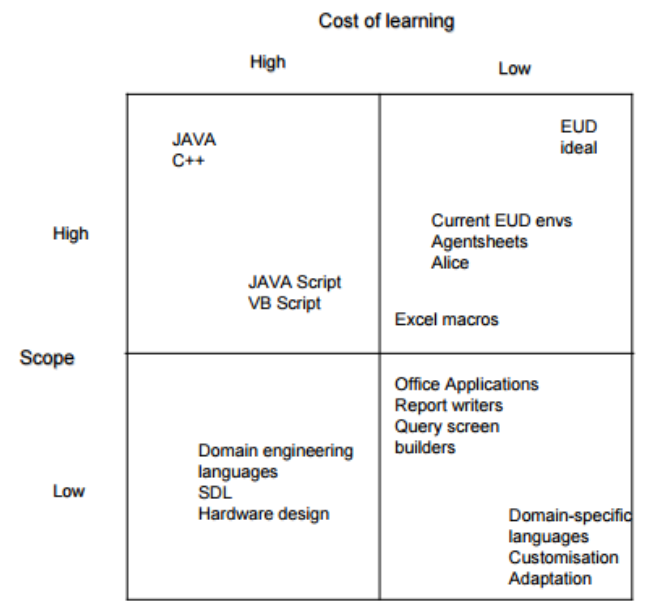
\includegraphics[width=0.7\textwidth]{bilder/chapter2/eudmatrix.png}
    \caption{Umfang des Anwendungsbereichs und Höhe des Lernaufwands unterschiedlicher \ac{EUD}-Werkzeuge gegenübergestellt.}
    \label{fig:kompvslern}
\end{figure}
Es gibt zwei Dimensionen, die bei der Erstellung eines \ac{EUD}-Werkzeug zu beachten sind: \textit{Anwendungsbereich} und \textit{Lernaufwand} (\cite{fischer2004meta}). In Abbildung \ref{fig:kompvslern} werden vier Quadranten gezeigt, welche Repräsentanten von Softwareerstellungs-Werkzeugen in ihrer Anwendungsbereich (Abbildungsvermögen des Werkzeugs) und ihrem Lernaufwand (zeitlicher Aufwand zum Erlernen des Werkzeugs) gegenüberstellt. Im Quadrant, der eine großen Anwendungsbereich abdeckt und einen hohen Lernaufwand an den Nutzer stellt, sind die klassischen Entwicklungswerkzeuge wie \texttt{C++} zu finden. Die Werkzeuge in diesem Quadrant sind nur meist nicht Domänen-gebunden und geben nur wenig Vorgaben unter welchem Paradigma sie verwendet werden müssen. Diese Flexibilität hat allerdings ihren Preis, den der Endnutzer muss über Monate und Jahre lernen, mit dieser Abstraktion umgehen zu können. Es existieren auch Werkzeuge mit einer wohl definierten Abbildungsvermögen (geringer Scope) und einer steilen Lernkurve. \acp{HDL} repräsentieren einen Vertreter dieses Quadranten. Ihre Komplexität geht einher mit der Einzigartigkeit der Domäne und der benötigten Spezialisierung des Endnutzers. \ac{EUD}-Werkzeuge sollten sich laut \cite{fischer2004meta} im Quadranten mit geringem Lernaufwand und großer Anwendbarkeit befinden. Ein solchen \ac{EUD}-Werkzeug ist allerdings nicht trivial umzusetzen. Wie schon im vorherigen Kapitel angesprochen, benötigen \acp{EUD}-Werkzeuge eine, auf die Domäne abgestimmte, Design-Metapher. Aus diesem Grund ist es fraglich ob ein solches, ideales \ac{EUD}-Werkzeug existieren kann.

\subsubsection{Cognitive Dimensions}
\begin{table}[h]
\centering
\begin{tabularx}{\textwidth}{lX}
\hline
\rowcolor[HTML]{EFEFEF} 
Dimension                 & Definition                                           \\ \hline
Viskosität                & Wiederstand gegenüber Veränderung                    \\ \hline
Sichtbarkeit              & Sichtbarkeit von Komponenten                         \\ \hline
Vorzeitige Festlegung     & Feste Vorgaben bei Interkationsreihenfolge           \\ \hline
Unsichtare Abhängigkeiten & Sichtbarkeit der Abhängigkeiten zwischen Komponenten \\ \hline
funktionale Aussagekraft  & Ersichtlichkeit der Funktionalität einer Komponente  \\ \hline
Fehleranfälligkeit        & Aktive/Passive Verhinderung von Fehlern              \\ \hline
Abstraktionen             & Qualität der Abstraktion von Datentypen/Komponenten  \\ \hline
Sekundäre Notation        & Zusätzliche Informationen unabhängig Notation        \\ \hline
Domänennähe               & Nähe der Design-Metaphern zur Domäne                 \\ \hline
Konsistenz                & Ähnliche Semantiken besitzen ähnliche Syntax         \\ \hline
Zerstreutheit             & Ausdrucksstärke der Notation                         \\ \hline
Mentaler Aufwand          & Kognitive Kosten der Notation                        \\ \hline
Endgültigkeit             & Finalität von Interaktionen                          \\ \hline
Vortwährende Evaluation   & Übersicht des eigenen Voranschreitens                \\ \hline
\end{tabularx}
\caption{Cognitive Dimensions laut \cite{blackwell2003notational}}
\label{tab:cognitivedimensions}
\end{table}
\acl{CD} ist ein in \cite{blackwell2003notational} vorgestelltes Framework um die Notation von (visuellen) Programmiersprachen zu bewerten. Nach \cite{blackwell2003notational} handelt es sich bei \ac{CD} nicht um eine konkrete Validierungsmethode, sondern vielmehr um ein Rahmenwerk von Vokabeln um die Usability einer Programmiersprache zu diskutieren. Vokabeln dieses Rahmenwerks werden kognitive Dimensionen genannt. In Tabelle \ref{tab:cognitivedimensions} kann eine vollständige Aufzählung sämtlicher kognitiver Dimensionen eingesehen werden. \ac{CD} verfolgt im Allgemeinen folgende Ziele:

\begin{itemize}
    \item Designer ermöglichen gezielte Aspekte (mit sich selbst) diskutieren und vergleichen zu können.
    \item Kompromisse und Schwerpunkte zwischen den verschiedenen Aspekten zu setzen.
    \item Erlaubt es durch groben Zügen über die Usability einer Sprache zu urteilen ohne sich in Detail zu verlaufen (''\textit{death by detail}'')
\end{itemize}

\ac{CD} schreibt laut \cite{blackwell2003notational} keine explizite Methode vor, wie verwendet werden soll. In der Praxis findet \ac{CD} als Basis von Fragebögen (z.B. \cite{EBobkowska.2003}, \cite{Wijayarathna.}) und als Grundlage für \textit{Cognitive Walkthroughs} (Evaluation anhand von Expertenmeinung, welche Handlungsabläufe innerhalb eines Werkzeuges durchspielen und bewerten) Verwendung (z.B. \cite{blackwell2000cognitive}). 

\begin{table}[h]
\centering
\begin{tabularx}{\textwidth}{lXX}
\hline
\rowcolor[HTML]{EFEFEF} 
Aktivität           & Definition                                                               & Beispiel\\ \hline
Suchen              & Finden von Informationen innerhalb der Notation                          & Finden eines Wertes innerhalb einer Tabellenzelle\\ \hline
Exploratives Design & Design eines Artefakts ohne einen festen Lösungsansatz                   & Live-Reloading, Skizzieren, etc.\\ \hline
Inkrementieren      & Hinzufügen von Informationen ohne die Struktur der Notation zu verändern & Hinzufügen von Funktionen zu einem Programm\\ \hline
Transkribieren      & Transformieren einer Information von einer Notation in eine Andere       & Kopieren einer Formel von einem Buch in eine Tabelle\\ \hline
Modifizieren        & Ändern einer Notationsstruktur ohne Informationen hinzuzufügen           & Layout einer Tabellenkalkulation ändern \\ \hline
\end{tabularx}
\caption{Aktivitäten innerhalb eines \ac{EUD}-Werkzeugs anhand \cite{green2000instructions}}
\label{tab:cogaktivitaeten}
\end{table}

Neben den in Tabelle \ref{tab:cognitivedimensions} definierten kognitiven Dimensionen, wird in \cite{green2000instructions} noch eine Reihe von \textit{User Activities} (Tabelle \ref{tab:cogaktivitaeten}) aufgezeigt. Diese Aktivitäten des \ac{EUD}-Werkzeugs erlauben dem Endnutzer, Softwareartefakte zu erstellen und zu modifizieren. Ziel dieser Aktivitäten ist es \textit{Trade-Offs} zwischen den kognitiven Dimensionen schärfer rationalisieren zu können. Beispielsweise ist die Viskosität beim Inkrementieren eines Wertes in den meisten Fällen sehr wichtig beim Suchen von Werten spielt es allerdings nur eine nebensächliche Rolle. 

\section{State-of-the-Art}\label{subsec:stateoftheart}
Im Folgenden werden populäre \ac{EUD}-Paradigmen untersucht. Da \ac{IoT} als Technologie noch selbst in einer frühen Entwicklungsphase befindet, ist die Anzahl von produktiv eingesetzten \acp{EUD} in diesem Bereich noch stark begrenzt. Im Folgenden werden \ac{EUD}-Ansätze, die für die \ac{IoT}-Domäne entworfen wurden, diskutiert.

\subsection{Programming-by-Demonstration}
\paragraph{Beschreibung} \acf{PBD} ist eine weit verbreitetes \ac{EUD}-Paradigma zum Programmieren von repetitiven Arbeitsvorgängen (\cite{cypher1993pbd}). Auch Programming-by-Example genannt, nimmt der Endnutzer eine Reihe von Arbeitsschritten innerhalb der verwendeten Software manuell vor. Diese Arbeitsschritte werden aufgenommen und von dem \ac{PBD}-System in einen Algorithmus transformiert. Dieser Algorithmus erlaubt es dem Computer autonom die gleichen Arbeitsschritte auf ähnlich strukturierten Datensätzen nachzuahmen. Dadurch wird erreicht, dass nicht Software-affine Endnutzer ohne das explizite Nutzen einer Programmiersprache oder \ac{GUI}, Algorithmen definieren können.

\paragraph{Funktionsweise} Wie in \cite{cypher1993pbd} beschrieben, ist das einfachste Beispiel für die Implementierung von \ac{PBD}-Systemen, ein Makrorekorder. Makrorekorder sind ein fester Bestandteil vieler weit verbreiteter Software-Systemen (bspw. Excel oder Adobe Photoshop). Sie erlauben es dem Nutzer repetitive Vorgänge aufzunehmen um Sie dann von der Software auf zukünftige Arbeitspakete replizieren zu lassen. Wie \cite{cypher1993pbd} hier anmerkt, sind solche Ansätze zwar einfach für den Endnutzer zu erlernen aber auch stark in ihrer Flexibilität und Ausdrucksweise eingeschränkt. In der Literatur gibt es verschiedene Ansätze diese Einschränkung mindestens partiell zu umgehen. Beispielsweise kann die Makro-Aufzeichnung als (visueller) Programmcode angezeigt werden. Dieser Programmcode kann dann vom Endnutzer modifiziert und generalisiert werden, um für eine größere Bandbreite von Datensätzen nutzbar zu sein.

\begin{figure}[h]
    \centering
    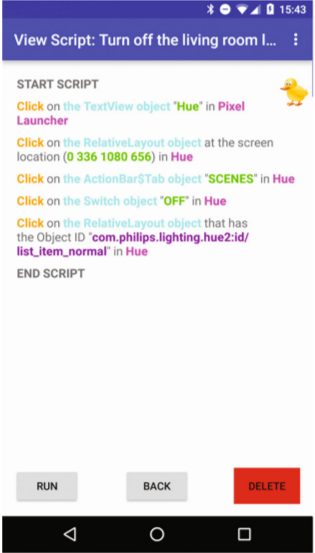
\includegraphics[width=0.3\textwidth]{bilder/chapter2/epidosite__example.png}
    \caption{\textit{EPIDOSITE}-Skript, das Interaktionen mit einer \ac{IoT}-Lampe beschreibt}
    \label{fig:epidositeexample}
\end{figure}

\paragraph{EPIDOSITE} Ein Beispiel für die Integration des \ac{PBD}-Paradigmas ist die, von \cite{li2017programming} vorgeschlagene, \textit{EPIDOSITE}-Plattform. Hierbei kann ein Makrorekorder, welcher auf einem Smartphone installiert ist, eine Abfolge von App-Interaktionen mit IoT-Systemen (bspw. Phillips Hue) aufnehmen. Einzelne Interaktionen können dann verkettet werden um komplexere Szenarien zu beschreiben. Grundsätzlich beschreibt der Endnutzer durch seine aufgenommenen Interaktionen \textit{Triggers} (dt. ''Auslöser/Bedingungen'') und \textit{Actions} (dt. ''Aktionen''). In einem Review-Prozess kann der Benutzer eine Skript (siehe Abbildung \ref{fig:epidositeexample}), welches der Makroaufnahme entspricht, überprüfen und gewünschte Änderungen vornehmen. Um die Interoperabilität und Funktionalität des Systems zu erhöhen lässt \textit{EPIDOSITE} dem Benutzer zu, virtuelle \textit{Services} über \textit{IFTTT} anzusprechen. 

\paragraph{Wertung} Der primäre \textbf{Vorteil} dieses Ansatzes ist der des \ac{PBD}-Paradigmas: ohne jegliche Programmierkenntnisse lässt sich ein \ac{IoT}-Systeme steuern bzw. im Verbund orchestrieren. Ein weiterer Vorteil von \textit{EPIDOSITE} bszw. \ac{PBD} sieht \cite{cypher1993pbd} darin, dass die Programmierung nicht von dem Interface, in der das Programm ausgeführt wird, getrennt ist (''\textit{Programming within the User Interface}''). Dieses Überlagern von \ac{EUD}- und Anwendungs-\textit{UI} reduziert die kognitive Dissonanz zwischen Entwicklung und Anwendung, welche bei Programmiersprachen vorherrscht. Somit erspart sich das \ac{PBD}-Paradigma in einfachen Anwendungen eine Abstraktionsebene. Als größte Herausforderung sieht \cite{cypher1993pbd} für \ac{PBD}-Systeme, die implizierte Absichten des Users herauszufinden. Selektiert man Beispielsweise in \textit{EPIDOSITE} die Temperatur eines Raums (um bspw. die Heizung einzuschalten) ist das \ac{EUD}-System erst einmal für unklar, welche genaue Bedingung der Benutzer damit verknüpft (''Heizung anschalten bei: kleiner 20°C? kleiner-gleich 20°C? etc.''). Des Weiteren stellen simple Makroaufnahmen sequentielle Programmabläufe dar. Um komplexere Konstrukte (komplexe Bedingungen, Umwandeln von Datensätzen, Schleifen) zu schaffen, welche in einem \ac{IoT}-Szenario durchaus vorstellbar sind, werden zusätzliche Funktionalitäten benötigt. Ein weiterer Nachteil, der von \cite{li2017programming} beschrieben wird ist, dass die Sichtbarkeit von Fehlern im Programmablauf stark eingeschränkt ist. Diese Undurchsichtigkeit schränkt die Usability des Werkzeugs eins. Des Weiteren fehlt \textit{EPIDOSITE} eine Möglichkeit erstellte Skripte zu simulieren. Würde der Benutzer eine Aktion an eine Bedingung an die Tageszeit knüpfen, müsste er die Uhr seines Smartphones verstellen um das Skript zu überprüfen. Dies erschwert das Programmieren von Aktionen, die an schwer manipulierbare Umgebungsvariablen (bspw. Temperatur, Helligkeit, etc.) gebunden sind.

\subsection{\acl{TAP}}

\paragraph{Definition} \ac{TAP} oder auch \textit{Rule-based Programming} stellt eine weitere, populäre Methode im \ac{EUD} für \ac{IoT}-Applikationen dar. Es handelt sich hierbei um ein stark vereinfachtes Programmierparadigma, welches dazu genutzt wird, Ereignisse zwischen mehreren Informationsquelle (z.B. Smart-Objects) zu lenken und sie somit kompositionieren (\cite{ur2014practical}). Bei \ac{TAP} spezifiziert der Endnutzer Sammlungen von Regeln, welche jeweils aus einer Aktion (Action) besteht, die vom System durchgeführt werden soll, falls ein Signal eintritt, das eine definierte Bedingung (Trigger) erfüllt. 

\paragraph{Funktionsweise} Ein typische \ac{TAP}-System besteht grundsätzlich zwei Elementen: Bedingung (Trigger) und Actions (Aktionen). Trigger können laut \cite{huang2015supporting} zwei Formen annehmen: Event (Einzigartig; bspw. ''Knopf wurde gedrückt'') oder State (Fortwährend; bspw. ''Die Sonne scheint''). Die resultierende Aktion kann ein Signal in drei verschiedenen Ausprägungen annehmen: Instant (analog zu Event), Sustained (analog zu State) und Extended (Temporär; bspw. ''Abschalten von Licht nach 2 Minuten''). Diese beiden Elemente (Trigger und Action) werden dann durch ein \ac{EUD}-Werkzeug auf visueller oder textueller Ebene zu Regeln zusammengefasst, welche zum Beispiel folgende Form annehmen:

\texttt{FALLS <Trigger -- Knopf wurde gedrückt> \\ UND <Trigger -- Nach 8 Uhr> \\ DANN <Action -- Schalte Licht für 5 Minuten ein>}

Die Komplexität des Triggers und der ausgelösten Action kann beliebige groß sein und ist primär abhängig von dem \ac{EUD}-Werkzeug und dem eingesetzten (\ac{IoT})-Kontext.

\paragraph{IFTTT - \textit{IF-THIS-THAN-THAT}} IFTTT ist ein populäres \ac{EUD}-Werkzeuge, das von vielen Endnutzern verwendet wird, um Prozesse zu automatisieren, die auch \ac{IoT}-Geräte involvieren. IFTTTs \ac{USP} ist ein stark vereinfachtes \ac{TAP}-Programmiermodell, welches sich, wie der Name IFTTT vermuten lässt, auf \texttt{IF <Trigger -- This> THAN <Action -- That>} beschränkt. Als Endnutzer hat \textit{IFTTT} Privateanwender im Sinn, welche die verstreuten \ac{IoT}-Ökosysteme miteinander kombinieren wollen.
\begin{figure}[h]
    \centering
    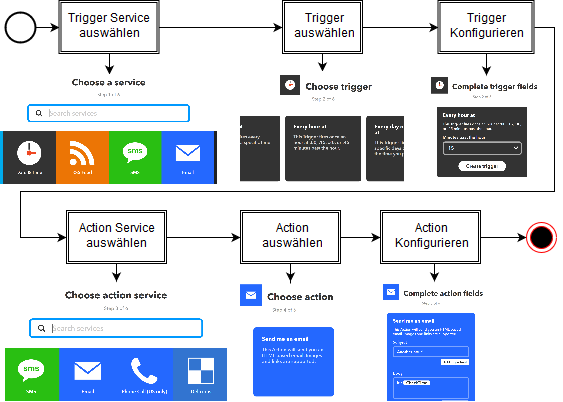
\includegraphics[width=0.9\textwidth]{bilder/chapter2/iftttproz.png}
    \caption{Der Erstellungprozess eines IFTTT-\textit{Recipes}}
    \label{fig:iftttprocess}
\end{figure}
 In Abbildung \ref{fig:iftttprocess} wird der Ablauf zur Erstellung eines IFTTT-Regelsatzes (gennant ''\textit{Recipe}'') dargestellt. Die Erstellung eines \textit{Recipe}, begrenzt sich auf sechs Schritte:
\begin{enumerate}
    \item \textbf{Trigger Service wählen}: Hier wird der Webservice oder das IoT-Gerät gewählt, welches die Quelle für das auszuwertende Trigger-Signal erzeugt. Beispiel: Tageszeit, Sonneneinstrahlung, Wetterdienst;
    \item \textbf{Trigger auswählen}: In diesem Schritt wird die Art des Trigger-Signals definiert. Beispiel für Tageszeit: Wenn X Minuten verstrichen, Jeden Xten Wochentag, von X Uhr bis Y Uhr;
    \item \textbf{Trigger konfigurieren}: Hierbei wird das vorher gewählte Trigger-Signal an die gewünschte Bedingung angepasst. Beispiel: Alle 45 Minuten, Jeden 3ten Wochentag, von 12 Uhr bis 14 Uhr;
    \item \textbf{Action Service wählen}: Analog zum ersten Schritt, wird hier der Konsument des Trigger-Signals in Form eines Webservices oder das IoT-Geräts gewählt. Beispiel: smarte Glühbirne, E-Mail Versand, Thermostat;
    \item \textbf{Action auswählen}: Auch hier wird gleich dem Trigger-Schritt, eine Aktion abhängig vom gewählten Konsument bestimmt. Beispiel: E-Mail versenden, E-Mail Postfach leeren;
    \item \textbf{Action konfigurieren}: Im letzten Schritt, wird die Aktion ausdefiniert. Hierbei werden Daten, die aus dem Trigger-Signal stammen verarbeitet. Beispiel: Sende die Nachricht mit dem Betreff: ''\textit{Es ist <Uhrzeit> Uhr}'';
\end{enumerate}
Aus dem in Abbildung \ref{fig:iftttprocess} gezeigten Recipe entsteht die Regel: Wenn 45 Minuten verstrichen sind, sende eine E-Mail mit dem Betreff: ''Es ist <Uhrzeit> Uhr''. Zwar besitzt eine solche Regel nur geringen Mehrwert, zeigt sie aber auch die Vielseitigkeit dieser Methoden, wenn bedacht wird, dass via IFTTT mehrere Hundert verschiedene Action und Trigger Services miteinander verbinden lässt. Triggers und Actions sind auf jeweils eine pro Recipe limitiert; es ist nicht möglich mehrere Trigger etwa mit bool'schen Operatoren zu verbinden. Auch State-Signale sind prinzipiell nicht statisch. Möchte man bspw. eine Lampe leuchten lassen, solange die Sonne mit Wolken verdeckt ist, muss man dieses \textit{Recipe} in zwei Regeln teilen: ''\textit{Anschalten wenn Wolken}'' und ''\textit{Ausschalten wenn Sonne}'' anstatt ''\textit{Solange Wolken, Lampe anschalten}''.

\paragraph{Bewertung} Der mit Abstand größte Vorteil von IFTTT im Vergleich zu anderen \ac{EUD}-Werkzeugen, ist die geringe Komplexität und vergleichsweise hohe Mächtigkeit. Dies wird dadurch erreicht, dass für eine Vielzahl von \textit{Services}, von professionellen Entwicklern Trigger-Signale und Action-Verhalten definiert wurden. Die Programmierung geschieht in natürlicher Sprache: ''\textit{Wenn dies, dann das}'' und ist daher auch für Laien sehr leicht verständlich. Diese vorteilhafte \textit{Usability} wird auch von mehreren Studien attestiert (\cite{huang2015supporting},\cite{ur2014practical}). 
Natürlich handelt es sich auch bei \ac{TAP} um keine ''\textit{Silver Bullet}'', die sämtliche Probleme von \acp{EUD} im Bereich \ac{IoT} löst. Das signifikanteste Problem ist die geringe Ausdrucksstärke von Regeln, die mit dem vereinfachten Programmierparadigma von bspw. IFTTT einhergeht (\cite{ur2016trigger}). Produkte die \ac{TAP} anwenden sind darauf bedacht, einen Mehrwert zu erzeugen, indem heterogene Systemenlandschaften verbinden können -- nicht aber programmatische Logik der einzelnen Komponente beschreiben. Des Weiteren, hat die Simplifizierung der Programmierung in IFTTT zur Folge, dass das Gefühl von persönlicher Weiterentwicklung mindert. Dies hat die Demotivation des End-Nutzers zur Folge hat (\cite{ur2016trigger}). Ein weiteres Problem ist laut \cite{huang2015supporting} die Mehrdeutigkeit \ac{TAP}-Regeln. Wie sich in der Studie herausstellte, werden selbst einfache Regeln von Nutzern unterschiedlich gedeutet, vor allem wenn eine Aktion eine temporäre Komponente besitzt. Beispielsweise wird ''\textit{Wenn es regnet dann...}'' von manchen Nutzern als ''\textit{Wenn es Beginnt zu regnen dann...}'' und von anderen als ''\textit{Solange es Regnet tue...}'' interpretiert. Das Erörtern solcher Unklarheiten wird zusätzlich erschwert, indem das Auffinden von Fehlern in Regeln von Werkzeugen wie IFTTT schlecht bis gar nicht unterstützt wird.

\subsection{Visuelle Programmierung}\label{subsubsec:samlabs}

\paragraph{Beschreibung} visuelle Programmierung ist per se keine \ac{EUD}-Technik sondern vielmehr eine abstrakte Darstellungsform für Programmcode. Visuelle Programmiersprachen (VPS) \acused{VPS} erlauben es dem Benutzer, durch die Erstellung und Manipulation von visuellen Objekten Programmcode zu generieren. Durch das Benutzen von visuellen statt textuellen Objekten, erhofft man sich, die Daten, Abläufe und Softwarefragmente für den End-Nutzer begreifbarer zu machen und somit die Benutzerfreundlichkeit als Ganzes zu verbessern (\cite{burnett2002software}). \ac{VPS} ermöglichen diese Begreifbarkeit durch die gezielte Verwendung von Metaphern: Blöcke, Röhren, Graphen, usw. sind alltägliche Elemente, welche sich durch ihre Verhalten, Struktur und Benutzung charakterisieren. Durch den gezielte Einsatz solcher Analogien, erhofft man sich das mentale Modell des Endnutzers zu prägen (\cite{Myers1986vis}). In der Praxis sind \acp{VPS} weit verbreitet: von der Erzeugung komplexer Funktionen (bspw. LabVIEW) über die Programmierung von Computerspiel Logik (bspw. Unreal-Engine Blueprint\footnote{\url{https://docs.unrealengine.com/en-us/Engine/Blueprints} -- besucht September 2018}), bis hin zur Steuerung von sowjetischen Raumfähren (bspw. DRAKON \cite{parondzhanov1995drakon}) unterstützen \acp{VPS} Domänenexperten, bei der Erstellung von Softwareartefakten. 

\paragraph{Funktionsweise} Eine einzige Funktionsweise für \ac{VPS} gibt es aufgrund der breit gefächerten Anwendungsgebiete nicht. Grundsätzlich erhofft man sich durch das Einführen zusätzlicher Informationsdimension (bspw. Position, Farbe, Animation), die Benutzerfreundlichkeit für den Endnutzer zu verbessern (\cite{Myers1986vis}). Es lassen sich allerdings verschiedene Aspekte identifizieren, welche prägend für das Design einer \ac{VPS} sind: Visualisierung von Kontrollfluss und/oder Datenfluss, des Programmzustands, Funktionsumfang und Programmstruktur (\cite{boshernitsan2004visual}). Grundsätzlich unterscheiden sich \acp{VPS} nicht von \acp{DSL}. Sie bestehen auch aus einer Syntax von Elementen und einer Semantik die den Elementen Sinn verleiht. Zusätzlich besitzen \ac{VPS} oftmals Pragmatismen -- unter ihnen versteht man spezielle Funktionalitäten zur Verbesserung der Usability; beispielsweise das manuelle modifizieren von Variablen zur Laufzeit des Programms (\cite{Repenning2017MovingBS}). Kernstück einer einer \ac{VPS} ist die Metapher, mit welcher der Programmcode abstahiert wird. 

\paragraph{SAM Labs/Studio} SAM Labs ist ein Bildungswerkzeug für \ac{IoT}. Es besteht -- ähnlich wie cBlocks -- aus einer Sammlung von separaten Sensor- und Aktorblöcken, welche kabellos miteinander kommunizieren. Jeder Block (Abbildung \ref{fig:samlabssub1}) besitzt nur eine Aufgabe: Fühlen von Temperatur, Auslesen von elektrischem Widerstand, Leuchten von LEDs, Abspielen eines Geräusches, etc. 

\begin{figure}[h]
\centering
\begin{subfigure}{.5\textwidth}
  \centering
  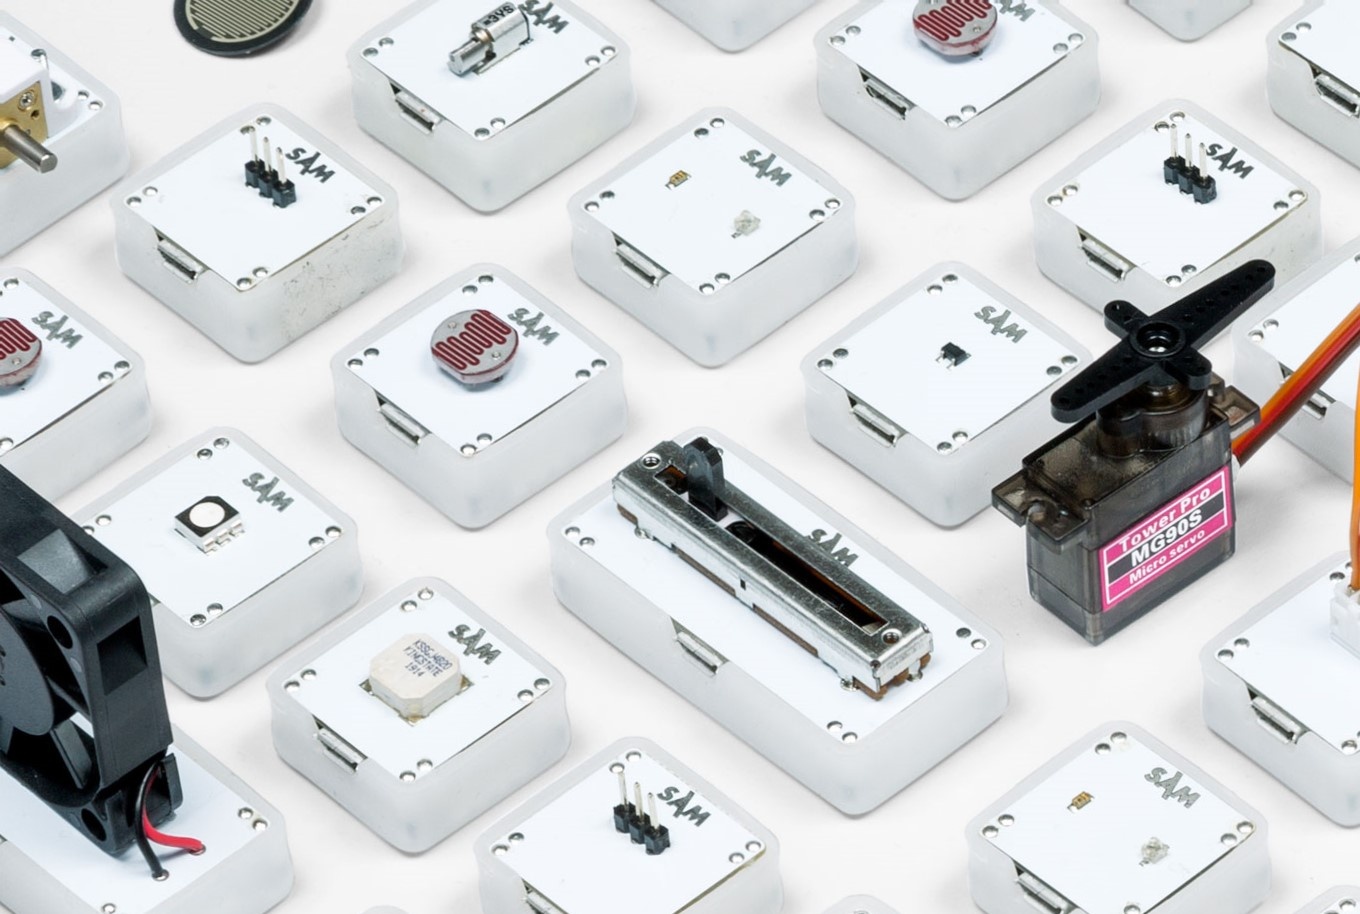
\includegraphics[width=.9\linewidth]{bilder/chapter2/samlabs.jpg}
  \caption{Eine Sammlung von SAM Labs Blöcken}
  \label{fig:samlabssub1}
\end{subfigure}%
\begin{subfigure}{.5\textwidth}
  \centering
  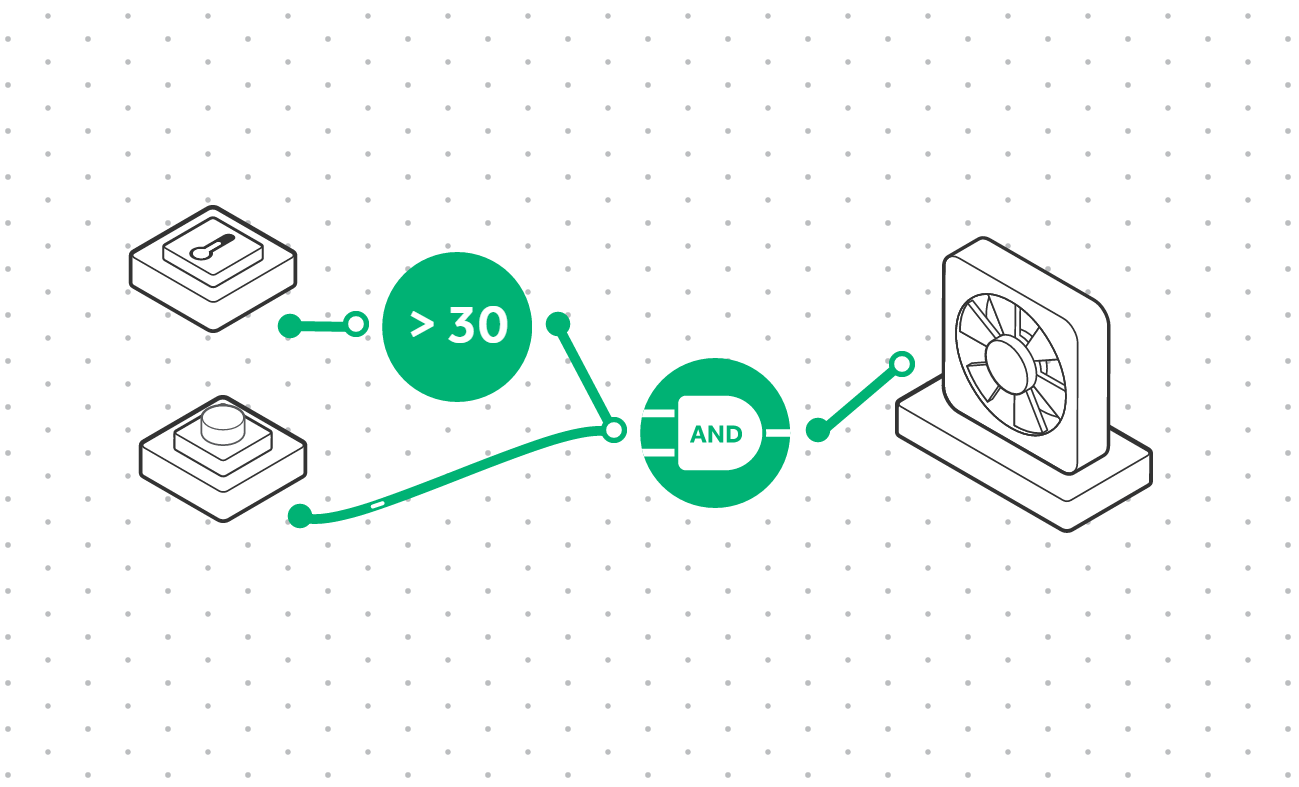
\includegraphics[width=.9\linewidth]{bilder/chapter2/samlabside.png}
  \caption{Beispielprogramm entworfen in Sam Studio}
  \label{fig:samlabssub2}
\end{subfigure}
\caption{Das SAM Labs Ökosystem besteht aus Funktionsblöcken (links) und der SAM Studio IDE zur Erstellung der Programmlogik (rechts)}
\label{fig:samlabs}
\end{figure}

Das \ac{EUD}-Werkzeug, welches Sam Labs Nutzern erlaubt Programme zu erstellen heißt \textbf{Sam Studio}. Kernstück bei der Programmierung stellen hierbei drei Arten von Nodes: Signalquellen (Sensoren, Interaktionen, etc.), Wandler (Bool'scher Operator, Arithmetischer Operator, etc.) und Signalkonsumenten (Webservices, Aktoren). Jede Node besitzt jeweils einen Input und/oder einen Ouput über welches die Node ein Signal sendet oder empfangen kann. Inputs und Outputs werden mit einer Drag-n-Drop Geste miteinander über Links verbunden werden. Diese Links stellen dauerhafte Kommunikationskanäle zwischen den Nodes dar, analog zu Funktionsaufrufen zwischen verschiedenen Objekten. Sensoren zeichnen sich durch ihre skeuomorphische Darstellung aus, der Existenz eines Outputs und dem Fehlen eines Inputs. Aktoren besitzen ebenso eine realitätsnahe Darstellung, allerdings umgekehrt zum Sensor kein Ouput, dafür aber einen Input. Wandler besitzen einen Input und Output und eine abstrakte Darstellung, welche zusätzliche Information zur Konfiguration dessen liefert. In Bild \ref{fig:samlabssub2} ist ein Beispielsprogramm, welches aus zwei Sensoren (Temperatur und Button), zwei Wandlern (Komperator und Bool'sches Gatter) und einem Aktor (Ventilator) besteht. Dieses simple Programm drückt folgende Logik aus: ''\textit{Solange Temperatur >30°C und der Schalter gedrückt ist, rotiere den Ventilator}''. Anzumerken an der Darstellung ist, dass es nicht ersichtlich ist, welche Daten zwischen den Nodes fließen ob dies Steuerungs- oder Datensignale sind, ist nicht erkenntlich. 

\paragraph{Beurteilung} Graphische Programmierschnittstellen genießen neben \ac{TAP} die höchste Popularität als \ac{EUD}-Werkzeug im \ac{IoT}-Bereich. SAM Studio ist hierfür ein prominentes Beispiel, an dem man die Vor- und Nachteile des Paradigmas erläutern kann. Der primäre und offensichtlichste Vorteil von visuellen Programmiersprachen liegt in der Darstellung selbst. Menschen haben eine visuelle Denkweise, daher ist es naheliegend Probleme und Lösungen auf einer visuellen Ebene darzustellen, statt einer textuellen. Visuelle Metaphern erlauben es Endnutzern Erfahrungen aus der realen Welt auf die Programmierung übertragen. In SAM Studio werden Links zwischen den datenverarbeiteten Elementen gezogen. Dies könnte man mit dem ziehen von Förderbändern zwischen materialverarbeitenden Maschinen in der reellen Welt vergleichen. Des Weiteren lädt SAM Studio durch das einfache Manipulieren und Kopieren von einzelnen Elementen ein, explorative Entwicklung zu betreiben. Darüber hinaus, erleichtert die Darstellung von SAM Studio das \textit{Debugging} von Prototypen. Hierfür werden Animationen verwendet, durch die sich der Datenfluss visuell nachverfolgen lässt. Ein Vorteil im Vergleich zu \ac{TAP}, ist die Darstellung paralleler Datenströme. Wie in Bild \ref{fig:samlabssub2} zu sehen ist, sind die asynchron Signale der Datenquellen graphisch nachvollziehbar. Diese verteilte Erzeugung und Verarbeitung von Events ist schwierig in textueller Form darzustellen. 

\ac{VPS} besitzt nicht nur Vorteile. Eine der prominentesten Kritiken gegenüber \acp{VPS} wurde von Peter L. Deutsch (\cite{MASON201368}) formuliert:

\begin{quote}
    ''\textit{The problem with visual programming is that you can’t have more than 50 visual primitives on the screen at the same time.}''
\end{quote}


Diese Kritik bezieht sich auf die relativ niedrige Informationsdichte von \acp{VPS} im Vergleich zu textuellen Programmiersprachen, wenn man davon ausgeht, dass maximal 50 visuelle Elemente auf einmal auf einen Computerbildschirm passen. Allerdings wurde diese Aussage zumindest Teilweise entschärft unter dem Gesichtspunkt, dass ähnliche Konzepte wie Komposition und Dekomposition von elementaren Komponenten, um komplexere Elemente zu schaffen auf \ac{VPS} übertragbar ist.

SAM Studio hat speziell noch folgende Nachteile:
\begin{itemize}
    \item \textbf{Geringer Funktionsumfang}: Der Funktionsumfang ist zweierlei begrenzt: zum einen, gibt es nur eine geringe Anzahl von SAM Labs Blöcke. Der Endnutzer hat dadurch nur eine begrenzte Anzahl von möglichen Sensordaten und Aktor-Aktionen zur Verfügung. Zusätzlich ist die Ansteuerung von Nodes hart vordefiniert. Der Lüfter aus Bild \ref{fig:samlabssub2} lässt sich nur binär ansteuern; möchte man bspw. die Lüfterdrehzahl analog regeln ist dies nicht möglich. Dies wird zusätzlich dadurch erschwert, dass keine Komponente von SAM Labs \textit{Open Source} ist und somit nicht anpassbar ist.
    \item \textbf{Vermischung von Datenfluss und Kontrollfluss} Die Link Metapher von SAM Studio ist nicht in allen Fällen konsistent. In manchen Fällen, wie in Bild \ref{fig:samlabssub2}, wird ein Kontrollfluss zur Steuerung des Lüfters modelliert. Allerdings können Links aber auch Datenflüsse darstellen, bspw. ist das übermitteln von Farbcodes zwischen einem Wandler und einem Aktor möglich. Solche Inkonsistenzen hemmen das Verständnis von Programmen in SAM Studio.
    \item \textbf{Fehlende Fehlerprävention} Grundsätzlich kann der Nutzer sämtliche Nodes miteinander verbinden. SAM Studio erlaubt es somit auch, unsinnige Kombinationen zu erzeugen (z.B. Farbcodes an Ventilator senden). Dies kommt gleich einer Programmiersprache ohne statische Typisierung. Fehlerprävention wird somit nicht betrieben und zwingt den Nutzer sein Programm erst zur Laufzeit manuell zu validieren.
\end{itemize}
Da es sich bei SAM Labs um ein Produkt für Schulkinder zwischen sieben und zwölf Jahren handelt, ist die extreme Simplifizierung des Programmiermodells nachvollziehbar. 

\subsection{Zusammenfassung}
Zusammenfassend ist zu sagen, dass es viele Möglichkeiten gibt \ac{EUD} für \ac{IoT} umzusetzen. Die Vielfalt an Ansätzen und die Fokussierung von Forschung (\cite{2015iseud}, \cite{2017iseud}, uvm.) auf dieses Thema ist Zeuge dessen Relevanz. Unabhängig der Ansätze, sind sich die Autoren einig, dass die immerzu wachsende Digitalisierung unseres Alltagslebens durch \textit{Smart Objects} einem Mangel an Softwareingenieuren gegenübersteht, welche die Nischenbedürfnisse von Endnutzern umsetzen können. \acp{EUD} erlauben es diesen Mangel durch benutzerfreundliche Programmierschnittstellen zu überbrücken.

Wie sich in den vorherigen Unterkapiteln ableiten lässt, kommt es bei dem Design von \acp{EUD}-Werkzeugen auf drei Kriterien an: Scope, Endnutzer und Anwendungsdomäne. Der \textbf{Scope}, welcher die Balance zwischen Abbildungsvermögen der \ac{EUD} und der Komplexität der Darstellung der Programmartefakte definiert, kann extrem Unterschiedlich sein. IFTTT und SAM Labs setzen ihr Hauptaugenmerk auf Simplizität in allen Bereichen legen. Dies lässt sich durch die Anwendungsdomäne der \ac{EUD}-Systeme erklären: SAM Labs ein Werkzeug ist, um die Grundlagen von \textit{MINT}-Bildung Schülern näher zu bringen (hoher Usability-Anspruch, geringer Funktionsumfang). An dieser Stelle ist allerdings anzumerken, dass auch \ac{EUD}-Werkzeuge existieren (bspw. LabVIEW\footnote{\url{http://www.ni.com/de-de/shop/labview.html} -- besucht September 2018}), die von Ingenieuren im Alltag verwendet um komplexe Transformationen von Daten visuell darzustellen (geringerer Usability-Anspruch, hoher Funktionsumfang). Der \textbf{Endnutzer} selbst ist natürlich ein weiteres zentrales Kriterium für das Design des \ac{EUD}. Der Endnutzer nimmt mit seinen Zielen, seinem technischen Verständnis und seinem mentalen Modell, Einfluss auf die Anforderungen des \ac{EUD}-Werkzeugs, hinsichtlich Darstellung und Komplexität. IFTTT beispielsweise versucht es mit seinem natürlichsprachlichen Ansatz und definieren möglichst viele Aktionen vor, um auch Nutzern programmieren zu ermöglichen, die keinerlei Interesse an der Programmierung selbst besitzen. Die \textbf{Anwendungsdomäne} selbst ist von großer Bedeutung für die Wahl des \ac{EUD}-Paradigmas. \ac{IoT}-Lösungen charakterisieren sich als Event-getriebene, parallele System, welche (physisch) geteilte Teilsysteme miteinander verbinden (siehe Kapitel \ref{subsubsec:wsan}). Während die Event-Komponente bei IFTTT durch Regeln dargestellt wird, verwendet SAM Labs eine Röhren-Metapher um den parallelen Daten- und Kontrollfluss zu visualisieren. Beide Darstellungsarten haben Vor- und Nachteile hinsichtlich abbildbarer Komplexität und Usability. Nicht jedes \ac{EUD}-Paradigma ist allerdings für die Anwendungsdomäne \ac{IoT} sinnvoll anwendbar. \ac{PBD} bspw. fokussiert sich darauf dem Computer sequentielle, repetitive Schritte, die der Endnutzer manuell ausführt, nachzuahmen. Die Anwendungsdomäne ist somit ein weiterer Grund, die Metapher der Darstellung sorgfältig zu wählen.

Eine \ac{EUD}-Umgebung sollte die oben genannten Punkte berücksichtigen. Im Falle dieser Thesis der Scope des Prototyping definiert, die \textit{Persona} des Endnutzers charakterisiert und die Anwendungsdomäne geklärt werden.



 % Externe Datei einbinden
\chapter{Analyse}\label{chapter:analyse}
Im folgenden Kapitel werden die  die Mängel, der im vorherigen Kapitel angesprochenen \ac{EUD}-Ansätze und sowie der Kontext dieser Arbeit analysiert. Aus der Analyse der Probleme und Bedürfnisse des zentralen Stakeholder, der Persona, werden Ziele abgeleitet die, die \ac{EUD} erfüllen soll. Diese Ziele werden mit einer Anzahl von praktischen Szenarios verdeutlicht aus welchen wiederum Anforderungen an das zu konzeptionierende \ac{EUD}-Werkzeug festgelegt werden.  

\section{Problemanalyse}\label{sec:problemanalyse}
Im vorherigen Kapitel wurde der Kontext der \ac{EUD}-Umgebung analysiert. Im Folgenden werden daraus die einzelnen Probleme analysiert, die es für die zu konzeptionierende \ac{EUD}-Umgebung zu lösen gilt.

\subsection{Parallel contra Sequentiell -- Datenfluss contra Kontrollfluss}
Wie in den vorherigen Kapitel beschrieben, lässt sich die Kommunikation zwischen den einzelnen Knoten eines \ac{IoT}-System als \textit{aperiodisch} und \textit{parallel} beschreiben. Sensoren in einem solchen Verbund senden abhängig ihrer Abtastraten, asynchron Informationen als Datenpakete über ein \textit{Shared Medium} zu Signalwandlern (engl. "`\textit{Transducer}"'). Dieses Verhalten beschreibt einen Datenfluss von Erzeuger zu Konsument. \ac{EUD}-Werkzeuge wie beispielsweise SAM Studio oder LabVIEW nutzen hierbei Datenflussdiagramme, um den Benutzer ein organisieren und transformieren von Datenströme zu ermöglichen. Die Datenströme werden im \acp{cBlock}-Ökosystem unner von Aktoren konsumiert. Da Aktoren zu jeder Zeit nur einen Zustand (engl. "`\textit{State}"') annehmen können (bspw. kann ein Motor sich nicht parallel in zwei Richtungen drehen), ist die Verarbeitung der Eingangsignale \textbf{sequentiell}, anhand eines definierten Kontrollflusses. Hier liegt ein zentrales Problem: während die Orchestrierung zwischen den Nodes anhand von parallelen Datenflüssen modelliert wird, stellt sich die Signalverarbeitung bei den Aktuatoren als ein sequentieller Kontrollfluss dar. Eine \ac{EUD}-Lösung für cBlocks muss demnach beide Paradigmen effizient abbilden können: das Orchestrieren und Transformieren von parallelen Datenströmen sowie das Modellieren von sequentiellen Verhalten von Aktoren.

\subsection{Signalpriorisierung}
Bei der Signalpriorisierung handelt es sich um das Verhalten eines Daten-Konsuments (bspw. Aktor), wenn zwei, in Konflikt stehende Nachrichten eintreffen. Dieses Problem kann im folgenden Szenario verdeutlicht werden:
\begin{quote}
Regel A: "`Wenn es 32°C heiß ist, dann lass die LED rot aufleuchten."' \\
Regel B: "`Wenn es regnet, dann lass die LED blau aufleuchten."'
\end{quote}
Es wird schnell klar, dass beide Regeln in Konflikt zueinander stehen. Sollte es regnen und 32°C heiß sein, ist nicht klar, welche Farbe die LED hat. Falls das System keinen klar definiertes Verhalten bei kollidierenden Signalen besitzt, fällt es in einen nicht vorhersehbaren Zustand. \acp{EUD}-Werkzeuge besitzen daher unterschiedliche Herangehensweisen dieses Dilemma zu lösen: bei IFTTT beispielsweise gibt die Reihenfolge der Regeln an, welche Regel angewandt wird, bei SAM Space überschreibt das neueste Signal, das Letzte. Auch andere Systeme, wie das explizite Definieren von Priorisierung ist erdenklich \cite{MacLaurin2011kodu}. Es muss nur in Anbetracht gezogen werden, dass ohne eine solche Regelung das System intransparent für den Endnutzer wird und eine Fehlersuche erschwert.

\subsection{Visualisierung von Daten}
\begin{quote}
    "`\textit{Visualize Data, not Code. Dynamic behaviour, not static structure}"' \\ -- Bret Victor, \url{www.worrydream.com}
\end{quote}
In \ac{IoT} sind Daten, Dreh- und Wendepunkt für das Design von Systemen: Daten werden an den Sensoren erhoben, von Wandlern transformiert und von Aktoren konsumiert. Es macht daher Sinn, den Fokus der Visualisierung auf die Daten selbst zu setzen. Das Problem hierbei ist eine sinnvolle Darstellung für die Daten und deren Transformation zu finden. Während IFTTT diese Schwierigkeit durch einen vereinfachten Scope weitestgehend umgeht, benutzt SAM Labs animierte graphische Elemente um den Kontrollfluss darzustellen. Beide \ac{EUD}-Systeme stellen nur bedingt die Datenflüsse über eine zeitliche Dimension dar, dies erschwert die Fehlersuche da das Verhalten des Programmartefakts schwerer nachvollziehbar ist. Für professionelle Software-Engenieure ist ein solches Visualisieren der Daten unabdingbar. Das Verwenden von Debugging-Werkzeugen, welche diese Visualisierung ermöglichen, beherrschen den Programmier\-alltag. Für eine \ac{EUD} stellt sich daher das Problem, wie dieses Daten visualisiert werden können um das Verhalten, und den State des Programmartefakts auch für Laien erklärbar zu machen. 

\subsection{Funktionsumfang contra Komplexität}
Ein Beweggrund für die Entwicklung der cBlocks, ist das geringe Maß an Komplexität, welches ähnlichen Produkte wie SAM Labs oder Sonys MESH\footnote{\url{http://meshprj.com/en/}, besucht Juni 2018} zulässt. Der Grund hierfür ist, dass diese und viele weitere Produkte, ihren Fokus auf die Vermittlung von \textit{MINT}-Wissen legen. Diese Produkte werden an vorgefertigte Szenarien gebunden, welche von den Endnutzern nachgebildet werden sollen. Im Kontext des freien Prototypings, wird allerdings schnell klar, dass diese Werkzeuge auf Soft- und Hardwareebene an ihre Grenzen stoßen. Beim Design eines \ac{EUD}-Systems muss deren möglichen Umfang an abbildbarer Programmlogik mit der Darstellungskomplexität ausbalanciert werden. In SAM Labs wird die gewählte Balance bei der Steuerung von Aktoren verdeutlicht. Hierbei wird das Verhalten von Aktoren auf Eingangssignale nicht selbst gesteuert. Vielmehr werden vorgefertigte Steuerungsblöcke verwendet, welche für jeden Aktor speziell vorgefertigt sind. Im Falle eines LED-Aktor währen dies Funktionen wie "`Farbe rotieren"' oder "`Helligkeit ändern"'. Dies erleichtert zwar die Programmierung, schränkt den Endutzer aber ein, sobald er für seinen Anwendungsfall speziellere Verhalten benötigt. Das Problem ist also, das bestehende Produkte nicht mit den erlernten Fähigkeiten des Endnutzers wachsen, sondern lediglich ein Einstieg in die Programmierung der \ac{IoT}-Domäne darstellen. Diese Werkzeuge werden (bewusst) obsolet, sobald ein Maß von Programmkomplexität erreicht wird. Ein daraus resultierendes Problem ist, das Werkzeuge wie SAM Studio nur bedingt den tatsächlichen Programmablauf abstrahieren und somit für die Programmierung relevante Konzepte relevante Konzepte (bspw. \textit{State-Machines} oder \textit{Event-Loops}) nicht vermitteln.

\subsection{Open Source}
Das Problem von geschlossenen/proprietären Systemen ist nicht nur für flowws relevant sondern auch für cBlocks ähnliche Projekte, die es erlauben \ac{IoT}-Produkte zu entwickeln. Bausätze wie SAM-Labs oder Sonys MESH sind weder auf Software- noch Hardwareebene erweiterbar. Dies schränkt den möglichen Funktionsumfang signifikant ein und macht eine Erweiterung und Fortentwicklung der Plattform abhängig vom Hersteller. Währenddessen, wurde das cBlocks-Projekt auch darauf ausgelegt, dass Endnutzer die Möglichkeit besitzen, das Ökosystem um eigene Blöcke zu erweitern. Dies verlangt der \ac{EUD}-Umgebung und Hardware ab, flexibel und erweiterbar zu sein. Es lässt sich vermuten, dass die Einschränkungen von bestehenden Werkzeugen aufgrund von Geschäftsmodellen existieren. Das Problem, welches hieraus resultiert ist, dass sie als Prototyping-Werkzeuge nur eingeschränkt verwendbar sind, da sich der Endnutzer dem Funktionsumfang des Werkzeugs anpassen muss -- umgekehrt, wie es sein sollte. Dies ist in einem Kontext, in dem eine \ac{EUD}-Umgebung als Vermittlungswerkzeug für generelles \textit{MINT}-Lehrmaterial dient verständlich, nicht aber, wenn Designer Prototypen in spezialisierten Anwendungsdomänen bauen müssen.

\section{Persona}\label{sec:persona}
Personas stellen die Verkörperung der Endnutzers dar, welche die cBlocks und somit auch die \ac{EUD} verwenden sollen. Da \textit{flowws} als ein Teilsystem des cBlocks-Produkts entwickelt wird ist es sinnvoll, die in \cite{weckbach2018cblocks} beschriebene Persona aufzugreifen. Im Folgenden werden zwei verschiedene Personas definiert, welche sich in der Komplexität ihrer Ziele, der Größe ihrer Expertisen und ihrem Charakter unterscheiden.

\begin{tcolorbox}[title={Persona \#1, Laura, 24, UX-Designerin},toptitle=3mm,bottomtitle=3mm, bicolor ,sidebyside,righthand width=3cm, sharp corners, boxrule=.4pt, colback=green!5, colbacklower=green!5, label=personalaura]
\begin{quote}
    "`\textit{Ich möchte meine Gedanken so schnell wie möglich greifbar machen.}"'
\end{quote}
    \textbf{Ziele:} 
    \setlist[1]{itemsep=-5pt}
    \begin{itemize}
        \item Arbeit produktiv verbringen, anstatt Werkzeuge zu erlernen
        \item Erstellung von \textit{Gadgets} für den privaten Gebrauch
        \item Erprobung der Benutzerfreundlichkeit von \textit{Smart-Device}-Prototypen
    \end{itemize}
    \textbf{Expertise:} 
    \setlist[1]{itemsep=-5pt}
    \begin{itemize}
        \item \ac{UX}-Design Prinzipien, graphische Konzeptualisierung
        \item Design-Thinking, Double Diamond, etc.
        \item Paper-Prototyping, Wizard-of-Oz, etc.
        \item Photoshop, Illustrator, Sketch, etc.
        \item Basiswissen in Arduino/C, Javascript
    \end{itemize}
    
    \tcblower
    
    
\includegraphics[width=\linewidth]{bilder/chapter3/laura.png}
\end{tcolorbox}
Die zwei maßgeblichen Stakeholder des Projekts sind Laura (Persona \#1) und Mark (Persona \#2). Ihre Gemeinsamkeit ist, dass sie in der selben Consulting-Firma angestellt sind die sich darauf spezialisiert hat, für Drittfirmen Case-Studies im Bereich Produktentwicklung zu erstellen. Der Berufsalltag beider besteht darin, moderne Design-Methoden wie Design-Thinking auf Probleme von Industriefirmen anzuwenden. Die Arbeit besteht hierbei aus kurzen Entwicklungszyklen, in denen mehrere Prototypen gebaut werden. Hierbei arbeiten beide Personas Hand-in-Hand um über mehrere Iterationszyklen hinweg, um einen finalen Produktprototypen zu erstellen.

Der Unterschied beider Personas sind ihre Pain-Points, Ziele und Expertiesen. Laura lässt ihre Erfahrung in User Experience in die Entwicklung von Produkt-Hardware einfließen. Markus Hintergrund ist technischer Natur. Er lässt seine Erfahrung in Elektrotechnik und Embedded-Entwicklung auf das Produkt Design einfließen. Beide Personas arbeiten somit im Tandem, um \ac{UX} und Hardware miteinander zu verschmelzen. Lauras größter Pain-Point hierbei ist, dass ein iteratives Entwickeln von funktionalen Prototypen, durch die enorme technische Komplexität von Embedded-Hardware gehemmt wird. Obwohl sie grundsätzliche Erfahrung mit Arduino besitzt, können selbst geringfügige Änderungen zu kryptischen Fehlern und unvorhergesehenen Verhaltensweisen des Prototypen führen. Hierbei assistiert Mark, ein Creative Technologist, der sich um 

\begin{tcolorbox}[title={Persona \#2, Mark, 28, Creative Technologist},toptitle=3mm,bottomtitle=3mm, bicolor ,sidebyside,righthand width=3cm, sharp corners, boxrule=.4pt, colback=green!5, colbacklower=green!5]
    \begin{quote}
        "`\textit{Mehrmals den selben Code schreiben ist leider Alltag}"'
    \end{quote}
    \textbf{Ziele:} 
    \setlist[1]{itemsep=-5pt}
    \begin{itemize}
        \item Besseres Verwenden von bestehendem Code
        \item Einfacheres Vermitteln von erzeugtem Code mit Designern
        \item Schnelles Iterieren von Prototyp-Generationen
    \end{itemize}
    \textbf{Expertise:} 
    \setlist[1]{itemsep=-5pt}
    \begin{itemize}
        \item Design-Thinking, Rapid-Prototyping
        \item Embedded Programmierung, Elektrotechnische Grundlagen, Software Engineering
        \item Visual Code, Eagle, UML, C, etc.
    \end{itemize}
    \tcblower
    
\includegraphics[width=\linewidth]{bilder/chapter3/mark.png}
\end{tcolorbox}

die technische Implementierung der Anforderungen kümmert. Seine Arbeit besteht darin, geeignete elektronische Komponenten zusammenszutellen, die benötigte Software aufzusetzen, Leiterplatten zu entwerfen und komplexe Programmlogik zu schreiben. Für ihn ist es frustrierend, wenn er viel Zeit in immer wiederkehrende Aufgaben, wie das Aufsetzen von generischen Hardwareblöcken, investieren muss. Alleine das Aufsetzen von kleinen funktionalen Prototypen mit nur wenigen Teilen kann durch Design, Erstellung und Fehlerkorrektur von Programmcode, mehr als einen Tag in Anspruch nehmen. Mark würde sich viel lieber mit der Entwicklung von komplexeren Systemen beschäftigen. Laura auf der anderen Seite, wäre es lieber, unabhängiger von Mark zu sein und sich auf die Erprobung funktionaler Prototypen fokussieren zu können, ohne viel Zeit für Elektronik und Software-Debugging zu verschenken. Kommunikation bzw. der Austausch von fachlichen Informationen zwischen den beiden Personas spielt hierbei eine Rolle.

Das Ziel von "`Profi"'-Projekt, cBlocks und in Folge dessen, flowws ist es, die Pain-Points der Personas zu mildern, indem sie auf ihre fachlichen Stärken bauen. 
\section{Vision und Ziel}
Die Vision hilft dabei, die Langzeitziele einer Software nicht aus den Augen zu verlieren (\cite{wiegers2013software}). Die Vision für flowws, beschreibt die gewählte mittel- bis langfristige Zukunft für das Projekt und erlaubt es, die Designentscheidungen zu begründen und zu lenken. Die Vision für flowws lautet wie folgt:
\begin{quote}
    \textit{flowws ist ein Werkzeug, das Designern ermöglicht sich in \ac{IoT} auszudrücken wie es ein Stift ihnen ermöglicht sich auf Papier auszudrücken; dadurch schnell, agil und ohne im Sumpf der Technologien zu versinken, funktionale Prototypen zu erstellen.}
\end{quote}

Die mittelfristigen Ziele des Projekts, welche diese Vision umsetzen sollen, lauten wie folgt: 

\begin{table}[H]
\caption{Ziel \#1: Ausdrucksstärke von flowws}
\label{tab:ziel3}
\begin{tabularx}{\textwidth}{lX}
\hline
\rowcolor[HTML]{EFEFEF} 
Ziel \#1:     & Z\#1 \\ \hline
Name          & Expressiv \\ \hline
Rationale     & Ein Programm in flowws soll dem Endnutzer schnell verständigen, was sein Zweck und Verhalten ist. Programmcode in seiner rohen Form ist in seiner Aussagekraft stark Abhängig von der Sorgfalt des Erstellers. In IoT Projekten, wie denen von Laura und Mark arbeiten viele Personen kooperativ miteinander. Deshalb ist es Wichtig, dass ein Programm, sich so gut wie möglich selbst erklären kann. \\ \hline
Fit-Kriterium & Laura und Mark sollen es beide möglich sein ein ihnen unbekanntes Programm innerhalb weniger Minuten (abh. von der Größe des Projekts) zu analysieren und eine zumindest wage Aussage treffen können über das Verhalten des Programms. \\ \hline
\end{tabularx}
\end{table}

\begin{table}[H]
\caption{Ziel \#2: Tempo bei der Entwicklung von Programmen}
\label{tab:ziel2}
\begin{tabularx}{\textwidth}{lX}
\hline
\rowcolor[HTML]{EFEFEF} 
Ziel \#2:     & Z\#2 \\ \hline
Name          & Schnell zu programmieren und zu modifizieren\\ \hline
Rationale     & Programmierung in IoT-Szenarien artet aufgrund Komplexität, nicht selten in Trial-and-Error-Vorgehen aus. Selbst minimale Modifikationen können zu unvorhergesehenen Verhalten führen. Schnelle, expermental-getriebene Entwicklung soll mit flowws machbar sein.\\ \hline
Fit-Kriterium & flowws unterstützt experimentelles Vorgehen des Nutzers. flowws erlaubt dem Nutzer in ein bis zwei Tagen einen vorläufigen Prototyp zu erstellen und in wenigen Minuten unterschiedliche Konfigurationen des Prototyps ausprobieren zu können. \\ \hline
\end{tabularx}
\end{table}

\begin{table}[H]
\caption{Ziel \#3: Erlernbarkeit von flowws}
\label{tab:ziel1}
\begin{tabularx}{\textwidth}{lX}
\hline
\rowcolor[HTML]{EFEFEF} 
Ziel \#3:     & Z\#3   \\ \hline
Name          & Schnell zu erlernen \\ \hline
Rationale     & IoT-Entwicklung benötigt ein immenses vertikales Wissen. Man benötigt Erfahrung in Hardware-naher Entwicklung, Programmiersprachen wie C, Elektrotechnik und Mikroelektronik. Während cBlocks dass erlernen der elektrotechnischen Fähigkeiten erleichtert, soll flowws die Barriere für Programmierung in IoT-Szenarien erleichtern. \\ \hline
Fit-Kriterium & Laura sollte es möglich sein, in weniger als ein bis zwei Tagen die Grundlagen von flowws zu verstehen und schon nach wenigen Stunden triviale Programme selbst beschreiben können. \\ \hline
\end{tabularx}
\end{table}




\begin{table}[H]
\caption{Ziel \#4: ''\textit{Grow-as-you-go}''}
\label{tab:ziel4}
\begin{tabularx}{\textwidth}{lX}
\hline
\rowcolor[HTML]{EFEFEF} 
Ziel \#4:     & Z\#4 \\ \hline
Name          & flowws wächst mit den Fähigkeiten der Nutzer \\ \hline
Rationale     & Viele \ac{EUD}-Systeme sind auf eine sehr eingeschränkte Domäne ausgelegt und daher, von ihrem Leistungsumfang stark begrenzt. Diese Einschränkungen sind für kreative Prozesse suboptimal. flowws soll durch gezielte Erweiterbarkeit in seiner Funktionalität mit den Fähigkeiten des Nutzer wachsen. \\ \hline
Fit-Kriterium & Das Ziel ist erreicht, wenn es Mark und Lisa möglich ist, flowws um wiederverwendbare Funktionen und Elemente, zu erweitern.  \\ \hline
\end{tabularx}
\end{table}

Ziel \#1-\#4 sind eine Dekomposition der Vision in einzelne verifizierbare Pakete. Die Ziele helfen, Anforderungen an das System zu stellen und grundsätzliche Designentscheidungen zu begründen.


\section{Szenarien}\label{sec:szenarien}
Im Folgenden werden drei Szenarien beschrieben die verschiedene Komplexität aufweisen und verschiedene Anforderungen gegenüber flowws stellen. Alle Szenarios bilden simple Situationen ab, welche in flowws modelliert werden sollen. Die Szenarios versuchen die Problemstellungen von (kap) aufzugreifen um dadurch zu Erfahren, wie flowws damit umgehen würde und welche Vor- und Nachteile sich dadurch abzeichnen. Des Weiteren dienen di Szenarios später zur Verifikation der Funktionstüchtigkeit von flowws und zu einem gewissen Grad zum Nachweis des Erreichens der Ziele. 

\subsection{Szenario S\#1: Lichtschalter}
Im ersten und einfachsten Szenario wird soll eine zeitgesteuerte Lampe ein und ausgeschaltet werden. Hierbei kommen zwei cBlocks zum Einsatz: ein Taster-cBlock und ein LED-cBlock. Der Ablauf ist wie folgt:
\begin{enumerate}
    \item Die Lampe startet initial in einem ausgeschalteten Zustand
    \item Der Nutzer betätigt ein Taster des Taster-cBlocks
    \item Der LED-cBlock leuchtet auf
    \item Nach eine vorbestimmten Zeitspanne schaltet sich LED-cBlock ab
    \item Bei nochmaliger Betätigung des Taster-cBlocks springe zum zweiten Schritt
\end{enumerate}
In diesem Szenario ist es die grundsätzliche Funktionsweise von flowws zu illustrieren. Hierfür wird ein sequentielle Abfolge von Aktionen, welche durch ein Event (Benutzerinteraktion) getriggert werden, durchgeführt. Zusätzlich erlaubt dieses Beispiel die Verständlichkeit und Benutzbarkeit des Konzepts von flowws am Endnutzer auf einem grundlegenden Level zu testen.

\subsection{Szenario S\#2: Ampelschaltung}
Das zweite Szenario stellt eine Ampel mit Füßgängerübergang vor. Hier kommen drei cBlocks vor: ein Taster, welcher die Fußgängerampel betätigt und zwei LED-cBlocks, welche die Ampeln symbolisieren. Der Ablauf wird im Folgenden beschrieben: 
\begin{enumerate}
    \item Verkehrsampel steht initial auf Grün - Fußgängerampel auf Rot
    \item Der Nutzer betätigt ein Taster des Taster-cBlocks
    \item Verkehrsampel schaltet nach X Sekunden auf Gelb
    \item Verkehrsampel schaltet nach X Sekunden auf Rot
    \item Fußgängerampel schaltet nach X Sekunden auf Grün
    \item Fußgängerampel schaltet nach X Sekunden auf Rot
    \item Verkehrsampel schaltet nach X Sekunden auf Grün
    \item Bei nochmaliger Betätigung des Taster-cBlocks springe zum zweiten Schritt
\end{enumerate}
Dieses etwas größere Szenario erweitert die Komplexität im Vergleich zu S\#1 um Interaktuator-Kommunikation. Die beiden Aktuatoren müssen sich hierbei über ihren momentanen Zustand (State) austauschen. Ähnlich wie S\#1 elaboriert auch dieses Szenario die Funktionalität und Ausdrucksstärke von flowws.

\subsection{Szenario S\#3: Terrarium}
Im dritten und letzten Szenario wird ein intelligentes Terrarium beschrieben welches auf Umgebungstemperatur und Feuchtigkeit reagiert und dem Nutzer über eine LED Hinweise über den Zustand liefert. Zusätzlich steuert ein Taster die Beleuchtung innerhalb des Terrariums, indem er ein öffnen des Terrariums detektiert. In Summe werden drei cBlocks benötigt: zwei LED-cBlocks, ein Temperatur/Feuchtigkeits-Sensor-cBlock und ein Taster cBlock.
\begin{enumerate}
    \item Wenn Temperatur $>30^{\circ}C$ dann lass LED-Rot aufleuchten
    \item Wenn Luftfeuchtigkeit $>80$ dann lass LED-Blau aufleuchten
    \item Wenn Klappe geöffnet wird löse Taster aus
    \item Wenn Taster aufgelöst dann stelle LED-Block auf 100\% Helligkeit
    \item Wenn Klappe geschlossen wird löse Taster aus
    \item Wenn Taster ausgelöst dann stelle LED-Block auf 0\% Helligkeit
\end{enumerate}
Dieses dritte Szenario die Verbindung von Event-fokusierter Programmierung von Verhalten mit sequentiellem Verhalten. Während die Signal-LED konstant auf asynchrone, aperiodische Events wartet ist die Beleuchtung durch die Öffnung des Terrariums eine sequentielle. Auch die Fähigkeit der Priorisierung von Signalen muss flowws hierbei unter Beweis stellen. Ebenfalls wie S\#1 und S\#2 versucht dieses Szenario Aufschluss über die Aussagekraft und Verständlichkeit von flowws gegenüber der Steakholder zu liefern.
\section{Anforderungen}
Dieser Abschnitt handelt über die funktionalen und nicht-funktionalen Anforderungen von flowws. Da es sich bei flowws um eine Konzeptarbeit handelt, wird der Fokus auf nicht-funktionale Anforderungen gelgt, welche Bedingungen an Benutzbarkeit, Transparenz und an die in Kapitel \ref{tab:cognitivedimensions} beschriebenen Cognitive Dimensions stellen. 

\subsection{Funktionale Anforderungen}\label{subsec:fanf}
\begin{table}[H]
\caption{Funktionale Anforderungen}
\label{tab:fanf}
\begin{tabularx}{\textwidth}{llX}
\hline
\rowcolor[HTML]{EFEFEF}
ID    & Name                       & Beschreibung \\ \hline
FA\#1 & Vergleichsoperationen      & Verechnung von reellwertigen Daten durch ($<,\leq,=,\neq,\geq,>$) möglich. \\ \hline
FA\#2 & Bool'sche Operationen      & Verechnung von bool'schen Daten durch ($\neg, \land, \lor, \oplus$) möglich. \\ \hline
FA\#3 & Zeitgestauerte Operationen & Zeitliche Manipulation von Signalen durch Verzögerung \\ \hline
FA\#4 & Auslesen von Sensordaten   & Kontinuierliches Auslesen von Sensordaten zur Weiterverarbeitung \\ \hline
FA\#5 & Ansteuern von Aktoren      & Ansteuern von Aktoren und Auslesen deren Zustände \\ \hline
FA\#6 & Programmierung von Aktoren & Verhalten von Aktoren ist programmierbar \\ \hline
FA\#7 & Konvertierung von Signalen & Konvertierung zwischen verschiedenen Wertebereichen (bspw. $\left [ 0;1,0 \right ] \rightarrow \left [ 10;37 \right ]$) \\ \hline
\end{tabularx}
\end{table}

\subsection{Nicht-funktionale Anforderung}

\subsubsection{Verständlichkeit}
\begin{table}[H]
\caption{NFN \#0}
\label{tab:nfn0}
\begin{tabularx}{\textwidth}{lX}
\hline
\rowcolor[HTML]{EFEFEF} 
NFN\#0        & Nichtfunktionale Anforderung \#0 \\ \hline
Name          & Paralleles und sequentielles Verhalten begreifbar machen \\ \hline
Beschreibung  & flowws ermöglicht dem Endnutzer, ein Verständnis von parallelen aperiodischen Ereignissen und sequentiellen Vorgängen, zu erlangen. \\ \hline
Rationale     & Parallele Programmierung ist selbst für Experten ein kognitiv anstrengender Prozess. Sie ist allerdings unabdingbar für den asynchronen, aperiodischen Kontext von cBlocks. Gleichzeitig benötigt der Endnutzer ein solides Paradigma um sequentielle Steuerung von bspw. Aktoren zu verstehen. \\ \hline
Fit-Kriterium & Ein Endnutzer muss in wenigen Stunden das parallele und sequentielle Verhalten von fertigen Programmen deuten und modifizieren können.\\ \hline
\end{tabularx}
\end{table}


\begin{table}[H]
\caption{NFN \#1}
\label{tab:nfn1}
\begin{tabularx}{\textwidth}{lX}
\hline
\rowcolor[HTML]{EFEFEF} 
NFN\#1        & Nichtfunktionale Anforderung \#1 \\ \hline
Name          & Daten und State sichtbar machen \\ \hline
Beschreibung  & Für den Endnutzer sollen die Daten, die das Programm verarbeitet und der Zustand indem sich das Programm befindet für den Endnutzer sichtbar sein. \\ \hline
Rationale     & Programmcode ist normalerweise statisch. Diese Darstellung ist gewöhnungsbedürftig, da Menschen visuell denken. Eine Darstellung von Daten und Zustand kann die Ausführung eines Programms für Laien vereinfachen. \\ \hline
Fit-Kriterium & Wenn Daten und Zustand in einer Weise sichtbar sind, dass das Verhalten eines Programms, in kurzer Zeit für den Endnutzer erklärlich ist. \\ \hline
\end{tabularx}
\end{table}

\subsubsection{Erlernbarkeit}
\begin{table}[H]
\caption{NFN \#2}
\label{tab:nfn2}
\begin{tabularx}{\textwidth}{lX}
\hline
\rowcolor[HTML]{EFEFEF} 
NFN\#2        & Nichtfunktionale Anforderung \#2 \\ \hline
Name          & Schneller erlernbar als gebräuchliche Programmiersprachen im \ac{IoT} \\ \hline
Beschreibung  & flowws soll für den fachfremden Endnutzer schneller erlernbar sein, als übliche Programmiersprachen, die im IoT Bereich verwendet werden (bspw. C).\\ \hline
Rationale     & Programmierprachen die im Embedded-Bereich verwendet werden, besitzen eine steile Lernkurve. Komplexe Paradigmen wie Speicherverwaltung oder Parallelität müssen über Monate trainiert werden, bevor man effektiv mit ihnen umgehen kann. \\ \hline
Fit-Kriterium & Wenn Laura an einem Tag lernt die Grundzüge von flowws deuten, nach einer Woche ein vorgefertigtes Szenario programmieren und nach einem Monat ihre eigenen Szenarios entwickeln kann, gilt die einfache Erlernbarkeit von flowws als erwiesen. \\ \hline
\end{tabularx}
\end{table}

\subsubsection{Bedienbarkeit}
\begin{table}[H]
\caption{NFN \#3}
\label{tab:nfn3}
\begin{tabularx}{\textwidth}{lX}
\hline
\rowcolor[HTML]{EFEFEF} 
NFN\#3        & Nichtfunktionale Anforderung \#3 \\ \hline
Name          & Schnelle modifzierung bestehender Programme unterstützen \\ \hline
Beschreibung  & Bestehende Programme sollen nicht nur leicht erfassbar für den Endnutzer sein, sondern auch effizient modifizierbar sein. \\ \hline
Rationale     &  Prototyping bedeutet experimentieren. Ein schnelles ändern der Programm-Parameter und Strukturen erlaubt es dem Endnutzer in möglichst wenigen Schritten verschiedene Versionen eines Programms auszuprobieren. Dadurch wird dem Endnutzer exploratives Entwickeln ermöglicht.\\ \hline
Fit-Kriterium & Parameter und Strukturen des flowws-Programmes sind zur Laufzeit änderbar. \\ \hline 
\end{tabularx}
\end{table}

\begin{table}[H]
\caption{NFN \#4}
\label{tab:nfn5}
\begin{tabularx}{\textwidth}{lX}
\hline
\rowcolor[HTML]{EFEFEF} 
NFN\#4        & Nichtfunktionale Anforderung \#4 \\ \hline
Name          & Prävention von Übersetzungszeit-Fehlern \\ \hline
Beschreibung  & flowws soll vermeidbare Fehler, wie Konflikte zwischen Datentypen, im Voraus unterbinden. \\ \hline
Rationale     & Um zügig in der Programmierung voran zu kommen, ist es besser Fehler zu vermeiden ist besser als sie beheben zu müssen. \\ \hline
Fit-Kriterium & Übersetzungszeitfehler (bspw. fehlerhafte Typisierung) werden präventiv verhindert.   \\ \hline

\end{tabularx}
\end{table}




\subsubsection{Änderbarkeit/Wartbarkeit}
\begin{table}[H]
\caption{NFN \#5}
\label{tab:nfn5}
\begin{tabularx}{\textwidth}{lX}
\hline
\rowcolor[HTML]{EFEFEF} 
NFN\#5        & Nichtfunktionale Anforderung \#5 \\ \hline
Name          & Erweiterung von flowws hinsichtlich Transducern/Sensoren/Aktuatoren \\ \hline
Beschreibung  & Experten und Endnutzer können neue Transducer/Sensoren/Aktuatoren in flowws integrieren und ihre Funktionalitäten für andere Enduser bereitstellen. \\ \hline
Rationale     & \ac{EUD}-Werkzeuge sind vorwiegend geschlossene Systeme. Sie wachsen nur vom Funktionsumfang wenn der Hersteller dies erlaubt. Das führt dazu, dass sie schnell an ihre Grenzen stoßen und als Produktivwerkzeug nicht mehr von Nutzen sind. \\ \hline
Fit-Kriterium & Die Anforderung gilt als erfüllt, wenn flowws durch Programmcode sich an neue, vorher nicht mögliche, Anforderungen anpassen kann. Dies geschieht, ohne dass der Endnutzern den Sourcecode verändern muss. \\ \hline
\end{tabularx}
\end{table}
 % Externe Datei einbinden
\chapter{Konzeption}\label{chapter:konzeption}
Die im vorherigen Abschnitt dargelegten Probleme, Motivationen und Anforderungen werden im folgenden Kapitel in ein Lösungskonzept gefasst. Dieses Lösungskonzept schlägt vor, beschreibt, analysiert und rationalisiert ein Programmierungskonzept, die benötigten Komponenten sowie deren Darstellungsform.

\section{Rationale}\label{sec:einleitungkonzept}
Im Folgenden werden grundsätzliche Entscheidungen für die Gestaltung des \ac{EUD}-Kon\-zepts auf Basis der Anforderungen getroffen. Zu diesem Zweck werden diese Entscheidungsalternativen aufgezählt, beschrieben und auf Basis ihrer Vor- und Nachteile ausgewählt und begründet.

\subsection{Optionen}\label{subsec:optionen}
In den vorherigen Kapiteln (Sektion \ref{subsec:stateoftheart} u. Kapitel \ref{chapter:analyse}) wurden die Qualitäten/eigenschaften von bestehenden \ac{EUD}-Lösungen in Form von Darstellung und Programmierparadigma diskutiert, sowie die Probleme und Anforderungen, die an das Projekt gestellt werden, analysiert. Aus der folgenden Arbeit resultieren zwei grundlegende Entscheidungen, die für das Konzept getroffen werden: die \textbf{Darstellungsform} des Programmcodes und das \textbf{Programmierparadigma} selbst. 

Für die Darstellungsform der Programmlogik innerhalb der \ac{EUD} kommen zwei Optionen in Frage:
\paragraph{Textuelle Darstellung} Hierunter zählen viele \textit{general-purpose} Programmiersprachen wie C, Java, etc. und spezifische \acp{DSL}. Instruktionen zur Verarbeitung von Informationen werden hierbei in einem Fließtext gespeichert bzw. dargestellt. Generische Programmiersprachen besitzen einen sehr hohen Abstraktionsgrad, da sie prinzipiell von ihrem Anwendungsdomäne losgelöst sind. \acp{DSL} sind wie der Name suggeriert vom Abstraktionsgrad wesentlich näher an der Anwendungsdomäne. Sie bilden einen Kompromiss zwischen Erlernbarkeit und Umfang der Anwendbarkeit \cite{green1991comprehensibility}.

\paragraph{Graphische Darstellung} In dieser Darstellungsform werden Programme durch Manipulation von graphischen Elementen und Symbolen erstellt. Durch die Verwendung von graphischen Elementen wird versucht eine Metapher zwischen der physischen Welt und der digitalen Welt zu erstellen. Die Anwendungsbereiche sind vielfältig; sie reichen von Pädagogik (z.B. Scratch) zu domänenspezifische Anwendungen (z.B. SAM Studio) zu \textit{general-purpose} Anwendung (z.B. Node-RED oder DRAKON). 

Aus den vorherigen Kapiteln haben sich zwei Programmierparadigmen im \ac{EUD} für \ac{IoT} als besonders relevant hervorgetan:

\paragraph{Regeln-basiert} Das Paradigma der Regeln-basierte Programmierung manifestiert sich in Form von \ac{TAP}. Hierbei werden eintreffende Signale, mit einem Datensatz von natürlich-sprachliche Regeln, auf ihre Wahrheit geprüft. Erfüllung der Regeln führen zur Erzeugung neuer Signale oder dem Auslösen von Aktionen. 
\paragraph{Datenfluss-basiert} Anders als bei Kontrollfluss-Paradigmen, wird hierbei ein Programm nicht als ein Set von Instruktionen angesehen, die sequentiell auf einen Satz von zentral gespeicherten Daten angewandt werden (\textit{Data at rest}/von Neumann Architektur), sondern die Daten selbst werden durch einen Graphen von statischen Instruktionen geleitet (\textit{Data in motion}). Funktionen, welche die Daten transformieren sind dabei \textit{Black Boxen}, welche sobald an sämtlichen Schnittstellen Daten anliegen, diese verarbeiten. Dieses Verhalten macht Datenfluss-basierte Programmierung, im Vergleich zu Kontrollfluss-Paradigmen inhärent asynchron und parallel \cite{johnston2004advances}.

\subsection{Beurteilung}
Im Anbetracht der Stakeholder, Anforderungen und Zielsetzung des Projekts werden im Folgenden die Vor- und Nachteile der jeweiligen Optionen aus Kapitel \ref{subsec:optionen} gegeneinander Abgewogen, um einen grundlegenden Konsens für das \ac{EUD}-Konzept fest zu legen.

Textuelle Darstellung ist aus gutem Grund, eine der am weit verbreitetsten Darstellungsformen von Programmcode. Dies hat vielerlei Gründe: zuallererst spricht für eine textuelle Darstellung die Informationsdichte und Deskriptivität von geschriebenen Sprachen. Mit nur wenigen Zeichen, lassen sich komplexe Konstrukte und Verhalten beschreiben. Ausdrücke wie ''\textit{Abstract}'' sind schwer visuell eindeutig darzustellen.  Gleichzeitig bedeutet diese Ausdrucksstärke aber auch, dass dem Benutzer das Erlernen eines großen, abstrakten Vokabulars zumutbar sein muss. Zusätzlich muss hier darauf hingewiesen werden, dass die Ausdrucksstärke von textuellen Programmcode immer von den Fähigkeiten und dem mentalen Modell des Entwicklers abhängig ist. Diese Eigenschaften decken sich nicht mit den Fähigkeiten von Laura.

Über Intuitivität und Flexibilität textueller Darstellung lässt sich nur schwer Pauschalisieren. Die Darstellung von parallelem Programmcode stellt sich allerdings als besondere Herausforderung dar. Solange Programmcode sequentiell ausgeführt wird, ist die kognitive Anstrengung für den Entwickler vergleichsweise gering; von links nach rechts von oben nach unten wird der Programmcode, wie beim manuellen Lesen, ausgeführt. Simultane, mehrschichtige Ausführung von parallelem Programmcode hingegen, entspricht nicht der Metapher des sequentiellen Lesens. Hierbei leisten multidimensionale graphische Darstellungen Hilfestellung für den Benutzer. Graphische Oberflächen haben allerdings noch weitere Vorteile: im Kontext von domänenspezifischer Softwareentwicklung können sie wie \acp{DSL} durch (visuelle) Metaphern leichter, Brücken zum Anwendungskontext, schlagen. Diese domänenspezifischer Darstellung ermöglicht es Domänenexperten, die nur wenig Erfahrung mit Programmierung haben, ihr Wissen trotzdem auf die virtuelle Welt zu übertragen. Diese Theorie wird dadurch gestützt, dass die erfolgreichsten visuellen Programmiersprachen (LabVIEW, vvvvv, etc.) stark in ihrer Darstellung mit der Anwendungsdomäne gekoppelt sind und klar abgesteckten Rahmenbedingungen hinsichtlich Funktionalität besitzen. Auch Kritik gibt es gegenüber visueller Darstellung von Programmcode. Das \textit{Deutsch-Limit} nach [\cite{begel1996logoblocks}] besagt, dass es kaum möglich ist mehr als 50 Elemente gleichzeitig auf einem Bildschirm anzuzeigen, ohne die Übersicht zu verlieren. Bei einer textuellen Darstellung ist dieses Limit aufgrund der großen Informationsdichte wesentlich höher.

Die Diskussion über Datenfluss-basierter und Regeln-basierter Programmierparadigmen wurde schon an anderer Stelle geführt. Stellvertretend für beide Paradigmen können die Vor- und Nachteile von IFTTT und SAM Studio in Kapitel \ref{sec:loesungsans} bzw. die Probleme dieser Ansätze in Kapitel \ref{sec:problemanalyse} nachgelesen werden. Grundsätzlich ist zu sagen, dass der größte Vorteil von Regel-basierten Paradigmen die intuitive Natürlichsprachligkeit der Programmierung. Nachteile beinhalten mangelnde Übersicht bei großen Mengen an Regeln, Diskrepanzen bei der genauen Deutung der Regel durch Endnutzer und mangelnde Ausdrucksfähigkeit von Regeln mit komplexen Sachverhalten. Auf der anderen Seite basieren Datenfluss-Paradigmen ebenso auf einer soliden, für den End-Nutzer visualisierbaren Metapher. Dies zeigt sich in der Nutzung des Paradigmas in vielen Werkzeugen mit denen Endnutzer ohne Erfahrung in Softwareentwicklung produktiv arbeiten müssen: vvvv\footnote{\url{https://vvvv.org/} -- besucht August 2018} (für Designer), LabVIEW\footnote{\url{http://www.ni.com/de-de/shop/labview.html} -- besucht August 2018} (für Mathematiker u. Elektronikingenieure), unreal blueprint\footnote{\url{https://docs.unrealengine.com/en-us/Engine/Blueprints} -- besucht August 2018} (für Spieledesigner), etc.\,. Der Fokus auf Daten und ihre Transformation ist eine Parallele zwischen Datenfluss-Programmierung und der Charakteristiken der \ac{IoT} bzw. \textit{Smart Devices}. Dies ist ein Grund für die Verbreitung des Paradigmas in dieser Domäne. Nachteilig ist die erhöhte Komplexität im Vergleich zu Regeln-basierten Ansätzen und der hiermit verbundene Lernaufwand für den Endnutzer.

\subsection{Entscheidung}
Es ist aus der Diskussion ersichtlich, dass es schwierig eine klare Entscheidung für Programmierparadigma und Darstellung des Programmcodes zu treffen. Es gibt viele weitere Vor- und Nachteile die man noch vortragen könnte, man muss allerdings bedenken, dass die Effektivität einer solchen Entscheidung hinsichtlich Benutzerfreundlichkeit/Erlernbarkeit/etc. sich erst \textit{a posteriori} beurteilen lässt. Dies hat auch damit zu tun, dass jede \ac{EUD} speziell für ein Szenario konzipiert wird und es somit nur wenige vergleichbare Arbeiten bzw. Erprobungen in \ac{IoT}-Bereich der \acp{EUD} gibt. Nichtsdestotrotz, wird sich an dieser Stelle für eine Datenflussparadigma mit graphischer Darstellung als \ac{EUD} für flowws festgelegt. Die Punkte die für die Wahl ausschlaggebend sind:
\begin{itemize}
    \item \textbf{Graphische Darstellung} Es gibt viele Werkzeuge wie vvvv oder Scratch die schon jetzt von Designern und anderen Endnutzern verwendet werden, um in anderen Domänen, visuell zu Programmieren. Die graphische Darstellung hilft durch geeignete Metaphern, die Domäne mit dem Programmcode zu verbinden und unterstützt dabei die visuelle Denkweise von Stakeholdern wie Laura ohne sie mit abstrakten Konstrukten zu belasten. Es wird sich dadurch erhofft, die Erlernbarkeit zu fördern (siehe \hyperref[tab:NFA2]{NFA\#2}).
    \item \textbf{Graphische Darstellung} Zum digitalen Entwickeln von Prototypen in flowws, werden die physischen cBlocks benötigt. Es ist somit naheliegend, dass man die Visualität der Realität auf die virtuellen Repräsentation abbildet. flowws soll durch diese Darstellung der Elemente,  die kognitive Last von Laura reduzieren. Diese Bindung von physischem und virtuellen Zustand soll die Anforderung  \hyperref[tab:NFA1]{NFA\#1} erfüllen.
    \item \textbf{Datenfluss-Paradigma} Das Datenfluss-Paradigma ist schwerer zu erlernen wie das natürlichsprachige Regeln-basierte Paradigma. Allerdings ist die Metapher näher an der Realität. Auf elektrotechnischer Ebene wandeln cBlocks physische Phänomene in digitale Signale um, transformieren sie in eine verwendbare Form und wandeln durch Aktoren diese Signale wiederum in physikalische Phänomene um. Dieser Datenfluss auf Basis von elektrischen Signalen kann effizient durch ein Datenfluss-Paradigma auf Programmcode-Ebene emuliert werden. Es wird sich davon versprochen, die Benutzbarkeit von flowws zu verbessern und die kognitive Dissonanz zwischen Elektro- und Informatikebene zu mindern.
    \item \textbf{Datenfluss-Paradigma} Datenflüsse lassen sich gut visualisieren und  geht deshalb Hand-in-Hand mit der graphischen Darstellung des Programmcodes. Dies kommt der Benutzerfreundlichkeit und Fehleridentifikation zu Gute. Durch das Paradigma und dessen Visualisierung wird sich erhofft, Parallelität leichter begreifbar zu machen (siehe \hyperref[tab:NFA0]{NFA\#0}).
\end{itemize}

Aus diesen Gründen wurde sich für eine \ac{EUD} mit graphischer Programmierung auf Basis des Datenflussparadigmas festgelegt.

\section{Programmiermodel}
In diesem Kapitel wird sich der Konzeption eines Programmiermodells auf Basis der Anforderungen (insbesondere \hyperref[tab:NFA0]{NFA\#0}) und der Entscheidungen aus dem vorhergegangenen Kapitel erstellt.

\subsection{Datenfluss-basierte Programmierung}\label{subsection:datenflussprog}
Prototypen, die mit cBlocks entwickelt werden essentiell ein Netzwerk von Sensoren, welche Daten versenden, diese in eine nutzbare Form verwandeln und von Aktoren konsumiert werden. Sie verhalten sich so, wie die in Kapitel \ref{subsec:characIot} beschriebenen \acp{WSAN}. Diese Form von Signal-Kommunikation ist ähnlich derer von \ac{DBP}. Die Definition  laut \cite{sousa2012dataflow} von \ac{DBP} ist:
\begin{quote}
    ''\textit{Die Programmierung anhand von Datenflüssen führt ein ein neues Paradigma ein, bei dem die interne Struktur eines Programmes mit einem gerichteten Graphen repräsentiert wird, ähnlich wie bei einem Datenflussdiagramm.} ''
\end{quote}

\begin{figure}[h]
\centering
\begin{subfigure}{.45\textwidth}
  \centering
  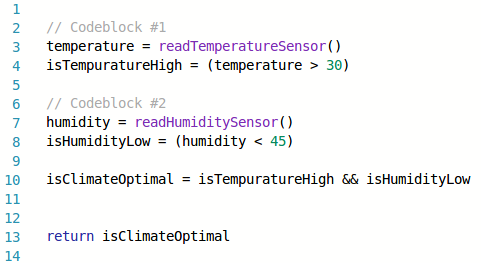
\includegraphics[width=1\linewidth]{bilder/chapter4/chapter4_2/codekbpbeispiel.png}
  \caption{}
  \label{fig:subvgldbptexttext}
\end{subfigure}%
\begin{subfigure}{.55\textwidth}
  \centering
  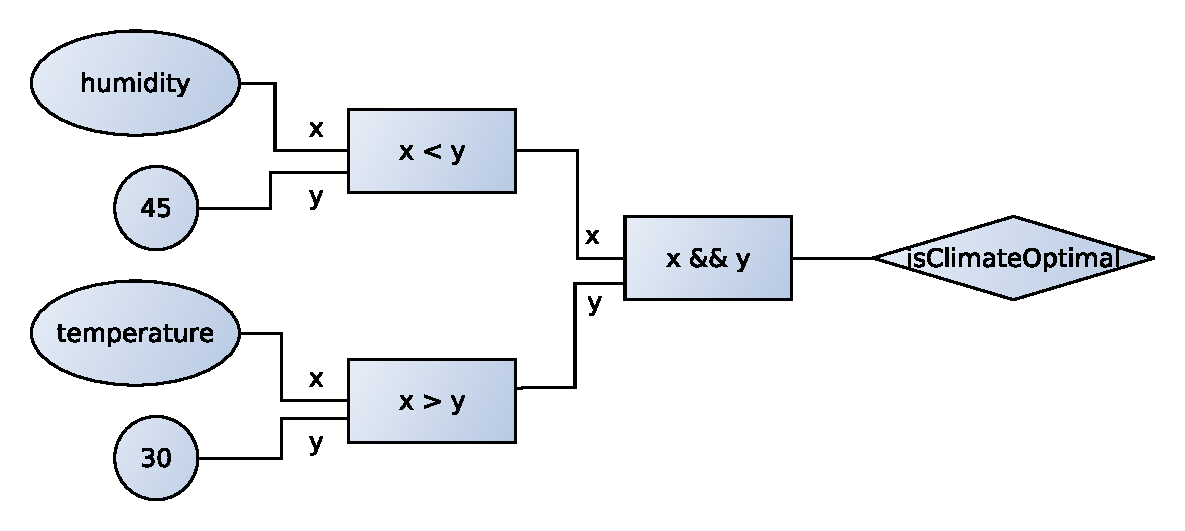
\includegraphics[width=1\linewidth]{bilder/chapter4/chapter4_2/beispieldatenfluss.pdf}
  \caption{}
  \label{fig:subvgldbptextdbp}
\end{subfigure}
    \caption{Der gleiche Programmcode in zwei Ansichten: \ac{KBP} (a) und \ac{DBP} (b). Hierbei ist die sequentielle Durchführung des \ac{KBP}-Modells mit der Parallelen des \ac{DBP} erkenntlich. Während beim linken Paradigma sequentiell die Blöcke abgearbeitet werden (wobei \#1 fertig sein muss um \#2 zu berechnen), ist das rechte Paradigma unabhängig von der Reihenfolge, in der die Signale eintreffen. Dies spiegelt den asynchronen Sachverhalt von \ac{WSAN} wieder.}
    \label{fig:bfd}
\end{figure}


Ein solches Programm wird in Abbildung \ref{fig:bfd} veranschaulicht. In dem konkreten Graphen handelt es sich um ein typisches Szenario, wie es mit flowws modelliert werden kann. Der Kontrollfluss-basierte Pseudocode zum selben Programm ist daneben zu sehen. In der Darstellung können vier verschiedene Elemente ausgemacht werden, die den Datenflussgraphen ausmachen. Die einzelnen Elemente, die mit dem Domänenmodel (Abbildung \ref{fig:bfddomainmodel}) korrespondieren sind:
\begin{figure}[h]
  \centering
  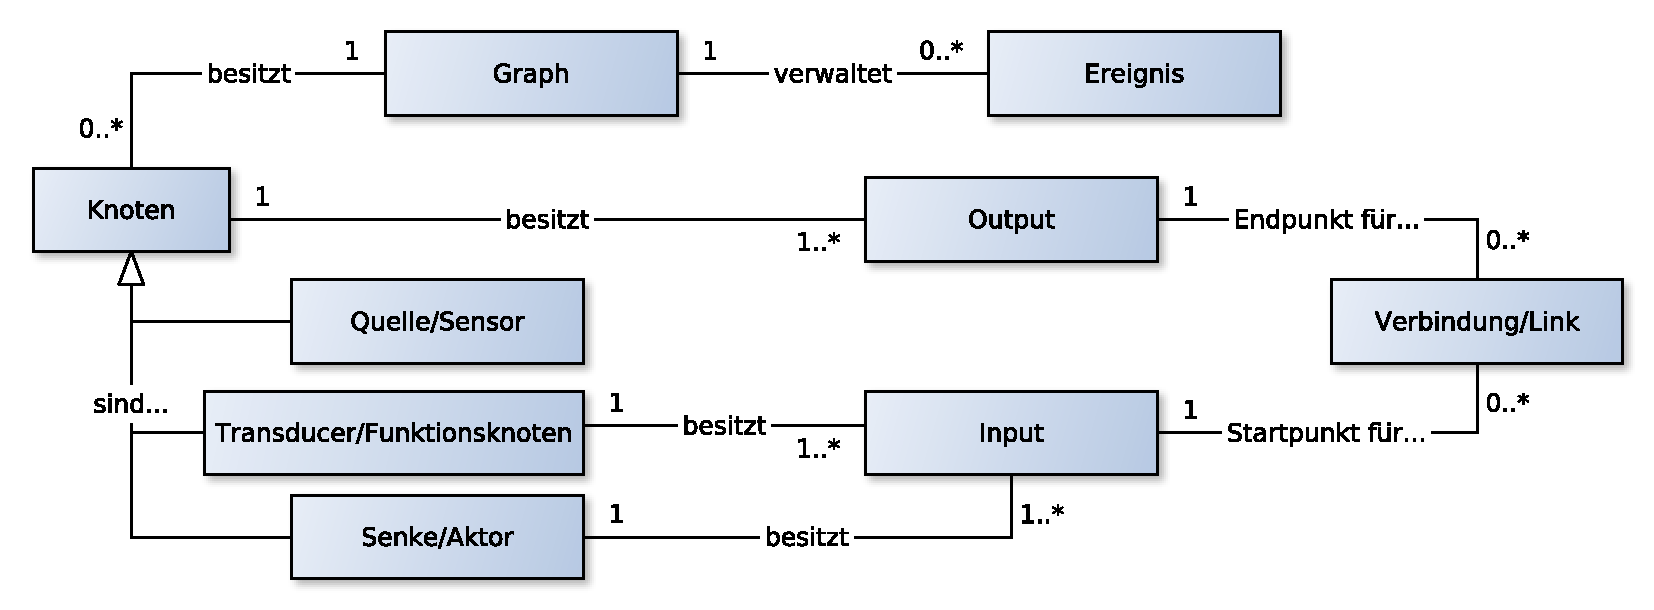
\includegraphics[width=0.95\textwidth]{bilder/chapter4/chapter4_2/domainmodelldatenfluss2.pdf}
  \caption{Das Domänenmodell des eines Datenflussprogrammes (in flowws) besteht aus drei Sorten von Knoten: Quellen/Sensoren, Senken/Aktoren und Funktionsblöcke/Transducer. Sie besitzen (mit Ausnahme der Quelle) Output- und Input-Interfaces, die es den Knoten erlauben durch Verbindungen/Links zu kommunizieren}
  \label{fig:bfddomainmodel}
\end{figure}
\begin{itemize}
    \item \textbf{Quellen} erzeugen die zu verarbeitenden Daten. Innerhalb von flowws bzw. cBlocks Netzwerken werden (virtuelle) Konstanten und (physische) Sensoren als datenerzeugendende Quellen angesehen. 
    \item \textbf{Funktionsknoten/Transducer} verarbeitenden Daten. Jeder Funktionsblock ist eine \textit{Black Box}, die aus einer Anzahl von Input-/Output-Schnittstellen und einer Verarbeitungslogik bestehen. Die Verarbeitungslogik wird im Falle von flowws von den funktionellen Anforderungen FA\#1 bis FA\#6 (Kapitel \ref{subsec:fanf}) vorgegeben. Nicht nur die Transformationen von Daten sondern auch temporale Operationen wie die zeitliche Verzögerung eines Signals werden in diesen Knoten abgearbeitet. 
    \item \textbf{Senken} konsumieren die erzeugten/verarbeitenden Daten. Innerhalb von flowws bzw. cBlocks Netzwerken übernehmen (virtuelle) Schnittstellen zu (physischen) Aktoren diese Aufgabe. Sie verwenden die erzeugten Daten, um ein bestimmtes Verhalten in Aktoren innerhalb des Systems herbeizuführen.
    \item \textbf{Verbindungen} transferieren Signale bzw. Nachrichten zwischen den Knotenpunkten. Sie definieren die eins-zu-eins Verbindung zwischen den Input/Output-Schnittstellen der Funktionsblöcke. Diese Verbindung ist gerichtet d.h. Daten fließen immer nur in eine Richtung durch den Graphen.
    \item \textbf{Ereignisse} sind Nachrichten, die durchd en Graphen von Node zu Node fließen. Sie beinhalten neben einem \textit{Payload}, der die eigentlichen Daten besitzt, auf dem die Transformationen durchgeführt werden, noch zusätzliche Metainformationen, die für die Bearbeitung der Daten wichtig sind. Die Datentypen, die der \textit{Payload} in besitzen kann wird von cBlocks-Ökosystem festgelegt und kann in Tabelle \ref{tab:datentypenpayloads} nachgeschlagen werden.
\end{itemize}

 \begin{table}[h]
\caption{Die drei verschiedenen Datentypen von Ereignis-\textit{Payloads}, die innerhalb von flowws verwendet werden.}
\label{tab:datentypenpayloads}
\begin{tabularx}{\textwidth}{llXX}
\hline
\rowcolor[HTML]{EFEFEF} 
Datentyp & Beispiel &  Erläuterung &  Verwendung \\ \hline
Number & 0,1,2,3.43,-12...& nummerischer Wert (Ganzzahlig und Fließkomma) & Temperatur, Abstand, Helligkeit, ...   \\ \hline
String & "qwnTZ32" & beliebige Zeichenkette & RFID-Code, Farbcodes, Display-Text, ... \\ \hline
Boolean & true, false & Wahrheitswert & Taster, Relays, ... \\ \hline
\end{tabularx}
\end{table}

\ac{DBP} erlaubt es effizient die Komplexität von parallelen \textit{Events} zu modellieren und auch für nicht Experten zu visualisieren. Dies ist somit ein guter Ansatz um die Anforderungen \hyperref[tab:NFA2]{NFA\#2} und \hyperref[tab:NFA0]{NFA\#0} zu bewältigen. Um \hyperref[tab:NFA0]{NFA\#0} allerdings komplett zu erfüllen, muss ein weiterer Sachverhalt adressiert werden: das modellieren sequentieller Logik, wie sie in Problem ''Parallel contra Sequentiell'' beschrieben und in  \hyperref[szenario2]{Szenario \#2} verdeutlicht ist.
\subsection{State-Machine-basierte Programmierung}\label{subsec:fsmprogrammierung}
\begin{quote}
    ''\textit{Have you tried turning it off and on again?}''  \\ -- Ein Jeder, der die Macht von \acp{FSM} verstanden hat.
\end{quote}

Bis zum jetzigen Zeitpunkt kann man den beschriebenen \ac{DBP}-Ansatz mit dem von SAM Labs (Kapitel \ref{subsubsec:samlabs}) vergleichen, auch mit seinen Problem (''Sequentiell contra Parallel'' und ''Signalpriorisierung''). Wie schon in den Problemen beschrieben, muss es Aktoren möglich sein mit parallel eintreffenden Signalen umgehen zu können, um Szenarien wie die in \hyperref[szenario2]{Szenario S\#2}  beschriebene Ampelschaltung und die in \hyperref[szenario3]{Szenario S\#3} beschriebene Vermeidung von Signalkonflikten zu ermöglichen.

Die einzige Möglichkeit für SAM Labs diesen Problemen aus dem Weg zu gehen ist es, sequentielle Logik mit der Datenfluss-Logik zu vermischen. Dies geschieht indem die Steuerungslogik der Aktoren, welche Entscheidungen über das Verhalten des Aktors treffen, auf der selben Ebene deklariert werden, wie die Logik, die Signale in eine nutzbare Form transformieren. In flowws wird einen anderen Weg gegangen. Es kommt eine Paradigma zum Steuern der Aktoren, welches weite Verbreitung in der IT und in \textit{Embedded Hardware} genießt: die \acl{FSM} (dt. ''endlicher Zustandsautomat'')

\begin{figure}[h]
  \centering
  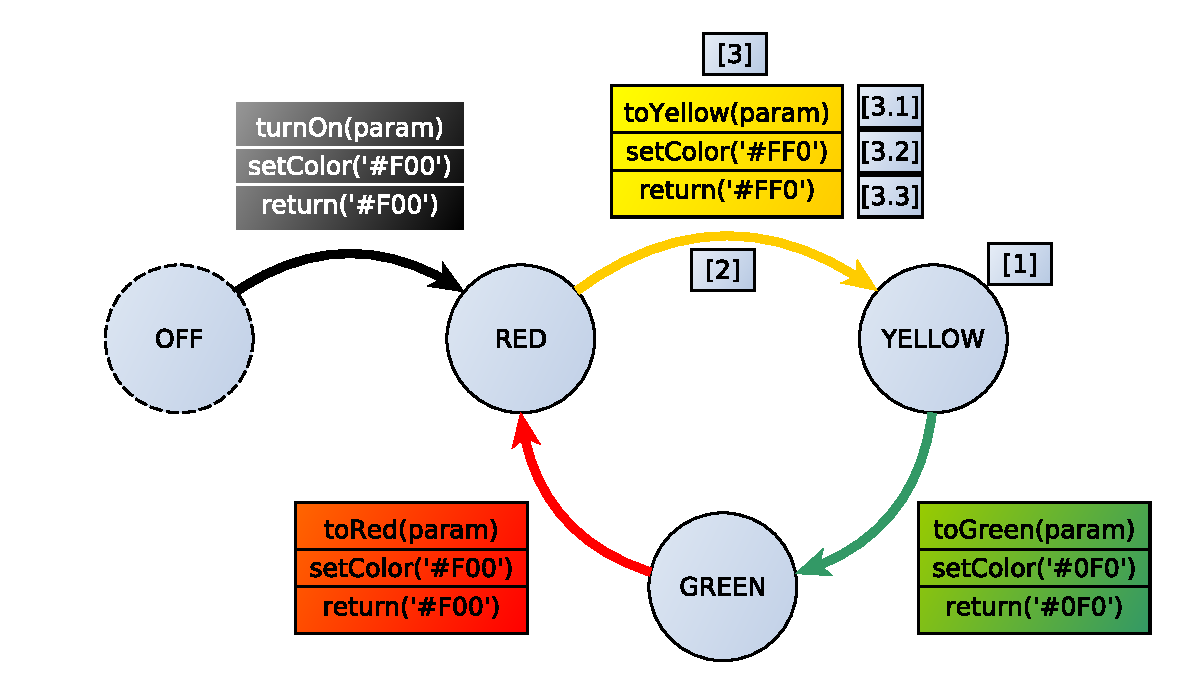
\includegraphics[width=0.85\textwidth]{bilder/chapter4/chapter4_2/beispielstatemachine.pdf}
  \caption{Die \ac{FSM} eines cBlocks mit LED-Aktor. Es existieren vier Zustände: OFF (Startzustand), RED, YELLOW, GREEN; und vier Übergänge: turnOn(), toYellow(), toGreen() und toRed(). Jeder der Übergänge verwendet in diesem Fall die setColor()-Funktion des LED-Aktors um die LED in der jeweils definierten Farbe wechseln. Jeder Übergang nimmt die Parameter (param) entgegen, was dem \textit{Payload} eines \textit{Events} entspricht. Dieser wird in diesem Beispiel entgegen genommen aber nicht verwendet. Zusätzlich erzeugt jeder Übergang mit return(<farbcode>) ein weiteres Event.}
  \label{fig:beispielfsm}
\end{figure}

\acp{FSM} sind Systeme von einer endlichen Menge von Zuständen (engl. ''States''), die auf eine endliche Menge von Ereignissen (engl. ''Events'') reagieren, welche außerhalb des Systems auftreten und auf das System einwirken. Die Reaktion einer \ac{FSM} auf eintreffende Signale werden abhängig einer endlichen Anzahl von Übergängen (engl. ''Transitions'') gesteuert. Wenn eine \ac{FSM} zu jeder Zeit nur einen Zustand annehmen kann, ist sie \textit{deterministisch} (\cite{hopcroft2013introduction}). 

Die Parallelen zu cBlocks bzw. flowws werden hierbei klar: cBlocks-Aktoren können als \acp{FSM} dargestellt werden. Ein Beispiel ist in Abbildung \ref{fig:beispielfsm} in Form eines LED-cBlocks gegeben, der eine Ampelschaltung modelliert. Es sind hierbei vier Elemente sichtbar, welche im Domänen-Modell (Abbildung \ref{fig:domainmodelfsm}) korrespondieren:
\begin{itemize}
    \item \textbf{Zustände/States [1]:} Ein Zustand drückt wie im \ac{FSM}-Modell den momentanen Status eines Automaten bzw. des Aktor-cBlocks aus. Diese Status ist nicht an die Ausprägung eines bestimmten Eigenschaft des Aktors gebunden, sprich ''RED'' bedeutet nicht zwangsweise die Farbe Rot. Vielmehr legt ein Zustand fest, welche zukünftigen Zustände beim eintreffen des nächsten Ereignisses erreichbar sind. In Abbildung \ref{fig:beispielfsm} ist es bspw. nicht möglich von Status ''RED'' in ''GREEN'' direkt zu springen. Durch dieses Konstrukt, lässt sich sequentielles Verhalten in den cBlock einprogrammieren. Zusätzlich existiert ein Anfangszustand, der die initiale Ausprägungen des cBlock-Aktors definiert.
    \item \textbf{Übergänge/Transitions [2]:} Die Übergänge werden ebenfalls durch den Nutzer definiert. Sie verbinden die einzelnen Zustände und modellieren das Verhalten eines cBlocks. Übergänge gestatten/verbieten durch ihre Existenz/Abwesenheit eine Signalpriorisierung vorzunehmen. Eine \ac{FSM} erlaubt es die Logik des cBlocks graphisch so zu modellieren, dass ein (zum momentanen Status) im Konflikt stehendes eintreffendes Signal ignoriert wird.
    \item \textbf{Übergangslogik/Transitional Logic [3]:} Die Logik, welche die Eigenschaften (Tabelle
\ref{tab:typesOfActutors}) eines Aktor-cBlocks manipuliert und somit physikalische Signale erzeugt, ist innerhalb der Übergänge. Sie besteht im Grunde aus drei Teilen:
    \begin{itemize}
        \item Die \textbf{Deklaration [3.1]} gibt den Namen des Übergangs an, der nach außen hin als Input-Schnittstelle sichtbar ist. Der Parameter der Deklaration symbolisiert den Payload, des eintreffenden Ereignisses und kann optional von der Funktionslogik weiterverarbeitet werden.
        \item Die \textbf{Funktionslogik [3.2]} beinhaltet die konkreten Instruktionen, die die Eigenschaften des cBlocks manipulieren. In Abbildung \ref{fig:beispielfsm} wird bspw. \texttt{setColor(<farbe>)} verwendet um die Farbe der LED zu ändern. Diese Funktionen sind für jeden Aktor speziell und werden von den cBlocks selbst vorgegeben. Experten (z.B. Persona ''Mark'') können allerdings weitere Funktionen hinzufügen und somit den Funktionsumfang eines Aktors für Laura erweitern.
        \item Der \textbf{Rückgabewert [3.3]} gibt ähnlich wie die Deklaration, eine Schnittstelle der Aktor-\textit{Black Box} an. In diesem Fall allerdings eine Output-Schnittstelle. Durch diese Schnittstellen kann ein Aktor seine Zustandsänderung, in Form eines neuen Ereignisses, dem Rest des Systems mitteilen. 
    \end{itemize}
\end{itemize}

\begin{figure}[h]
  \centering
  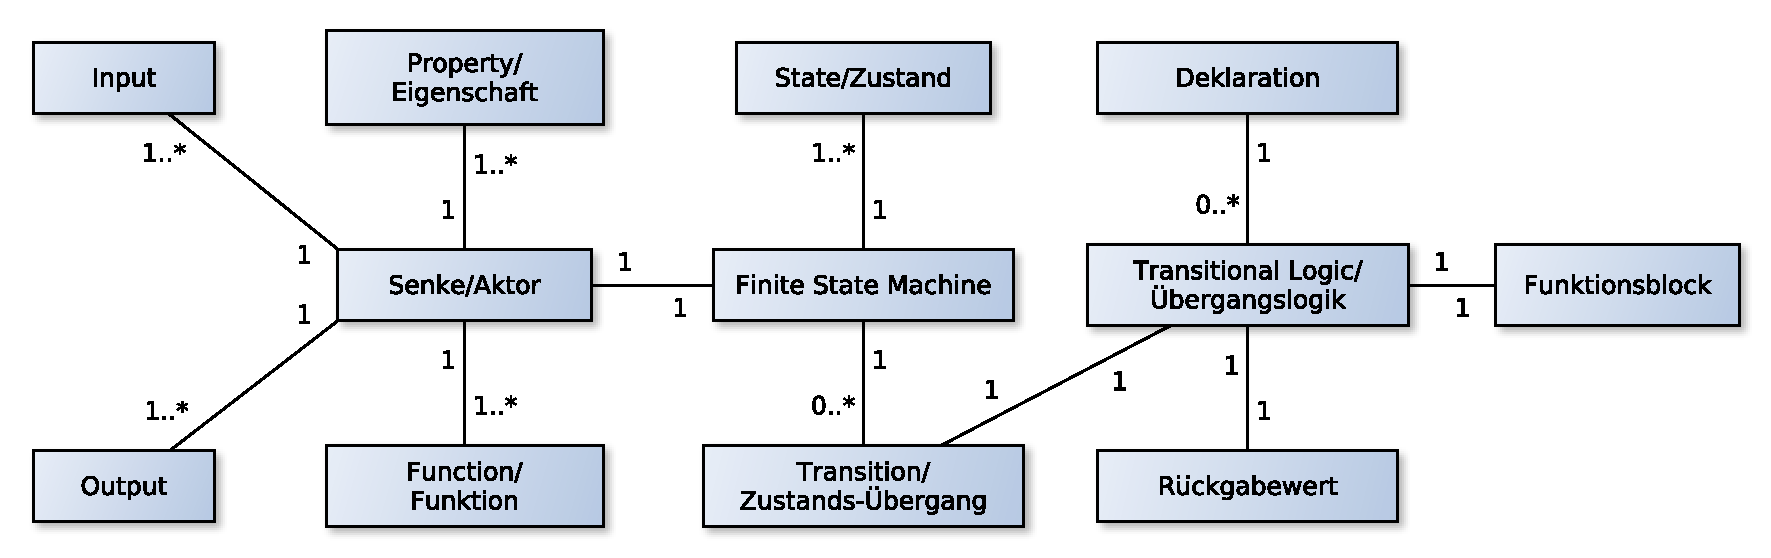
\includegraphics[width=1\textwidth]{bilder/chapter4/chapter4_2/domainmodellaktor.pdf}
  \caption{Das Domänenmodell des Aktors bzw. der \ac{FSM} ist eine Detailansicht von Abbildung \ref{fig:bfddomainmodel} hinsichtlich der Bestandteile des Aktors. }
  \label{fig:domainmodelfsm}
\end{figure} \hyperref[]{}

Durch das Verwenden einer \ac{FSM} ergeben sich mehrere Vorteile. Durch die gute Visualisierung der \ac{FSM} und der weiten Verbreitung des Modells kann die Erlernbarkeit gefördert und somit \hyperref[tab:NFA2]{NFA\#2}, adressiert werden. Zusätzlich erlaubt das Benutzen von \ac{FSM}, wie in  \hyperref[tab:NFA0]{NFA\#0} gefordert, sequentielles Verhalten zu modellieren, indem es die asynchronen Ereignisse, die auf den Aktor-cBlock einwirken, sequentiell zu verarbeiten. Das Hinzufügen von zusätzlichen Aktor-Funktionen durch Experten, kann das System nachträglich erweitert werden, wie es von  \hyperref[tab:NFA5]{NFA\#5} verlangt ist. Im nächsten Schritt muss geklärt werden, wie \ac{DBP} und \ac{FSM} miteinander integriert werden, um Endnutzern das Entwickeln von Programmen innerhalb von flowws zu ermöglichen.
\subsection{flowws}
In den zwei vorangegangenen Kapiteln wurden die zwei Paradigmen beschrieben, welche die Anforderungen bezüglich des Programmiermodells erfüllen sollen, namentlich die sequentielle und parallele Programmierung der cBlocks in visueller Form. Im Folgenden, wird das Zusammenspiel beider Paradigmen erklärt. Dabei wird auf das Konzeptmodell, Ausführungsmodell und die Eigenheiten von flowws bezüglich des cBlocks-Kontext eingegangen. Dieses Modell und die visuelle Darstellung sind die zentralen Bestandteile von flowws.

\begin{figure}[h]
  \centering
  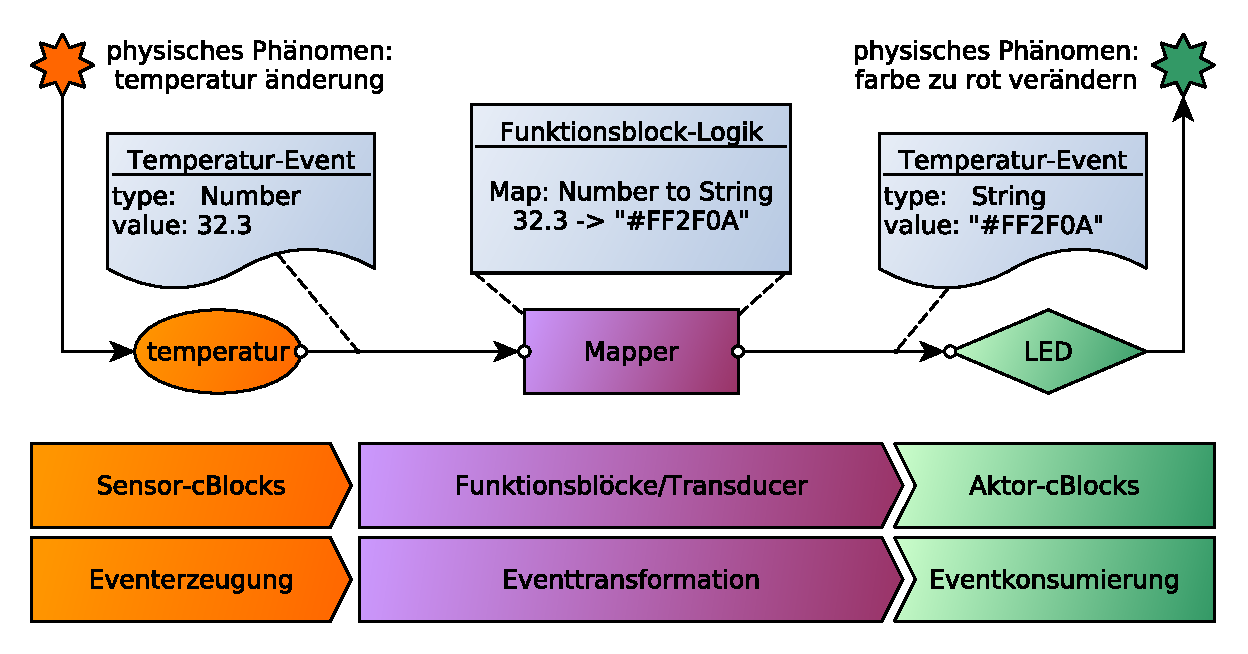
\includegraphics[width=1\textwidth]{bilder/chapter4/chapter4_2/flowwsschematicexample.pdf}
  \caption{Ein schematisches Beispiel für das Ausführungsmodell von flowws. Die Daten fließen von der Erzeugung als Events durch Funktionsknoten um zu transformiert zu werden. Dadurch erhalten sie einen höheren semantischen Wert, sodass sie vom Aktor konsumiert werden können.}
  \label{fig:beispielflowws}
\end{figure}

In Abbildung \ref{fig:beispielflowws} wird ein in flowws modelliertes Programm bzw. Graph schematisch dargestellt.  In diesem Beispiel, wird von einem Temperatur-Sensor ein Temperatur-Event erzeugt, welches die Farbe der LED manipulieren soll (blau für kalt, rot für warm). Hierbei wird ein Funktionsknoten verwendet, der den \texttt{Number}-Wert des Events auf eine Wertebereich von Farben abbildet. Dieses semantisch höherwertige Event wird dann vom Aktor bzw. der \ac{FSM} des Aktors verwendet, um dessen Zustand zu ändern. Hierbei wird das Kernprinzip von flowws, das sich in in drei Schritte aufteilt, verdeutlicht:

\subsubsection{1. Eventerzeugung}
 Eventerzeugung ist die erste Phase jedes flowws-Programmes. Jeder Sensor-cBlock, der mit dem System verbunden ist, besitzt einen virtuellen Sensorknoten als Repräsentant. Jeder Sensorknoten entspricht einem cBlock, d.h. cBlocks die mehrere unterschiedliche Events erzeugen (bspw. ein cBlock der Temperatur und Luftfeuchtigkeit misst) werden als einen Knoten mit mehreren Ausgängen dargestellt. 
 
 Wie in Abbildung \ref{fig:seqsensorblock} gezeigt, erzeugen Sensorknotens kontinuierlich Ereignisse mit Rohdaten als \textit{Payload}, auf Basis physikalischer Phänomene (z.B. Temperaturschwankungen). Diese Rohdaten haben oftmals keine semantische Bedeutung und sind in vielen Fällen schlichtweg Zahlenwerte oder Zeichenketten (siehe Tabelle \ref{tab:datentypenpayloads}).
 
 \begin{figure}[h]
  \centering
  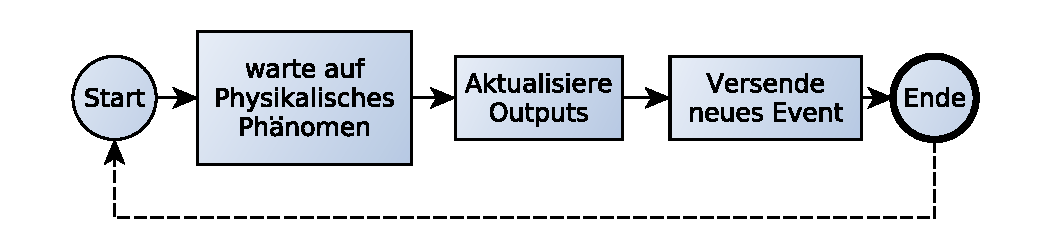
\includegraphics[width=1\textwidth]{bilder/chapter4/chapter4_2/sensorblockablauf.pdf}
  \caption{Standardablauf innerhalb eines Sensorknotens, wenn ein physikalisches Ereignis erfolgt ist.}
  \label{fig:seqsensorblock}
\end{figure}

 Wie alle anderen Knoten innerhalb von flowws sind auch Sensorknoten \textit{Black Boxen}. Der Unterschied zu anderen Knoten ist allerdings, dass sie keine Eingänge besitzen, sondern ausschließlich Ausgänge als Schnittstellen, da sie selbst nicht in ihrem Verhalten beeinflusst werden sollen. Dies soll die Verbindung zum physikalischen Sensor cBlock stärken, da es intuitiv ist, dass Aktoren ein aktives Verhalten besitzen während Sensoren passiv ihre Umgebung wahrnehmen. 
 
 \subsubsection{2. Eventtransformation}\label{subsubsec:eventtrans}
 Bei der Eventtransformation kommt dass \ac{DBP}-Paradigma aus Kapitel \ref{subsection:datenflussprog} zu tragen. Die erzeugten Daten werden durch eine Reihe von Funktionsknoten geleitet und somit miteinander kombiniert und/oder transformiert. 
 
 Der Ablauf einer Transformation innerhalb eines Funktionsknotens ist in Abbildung \ref{fig:seqfunktionsblock} dargestellt.
 \begin{figure}[h]
  \centering
  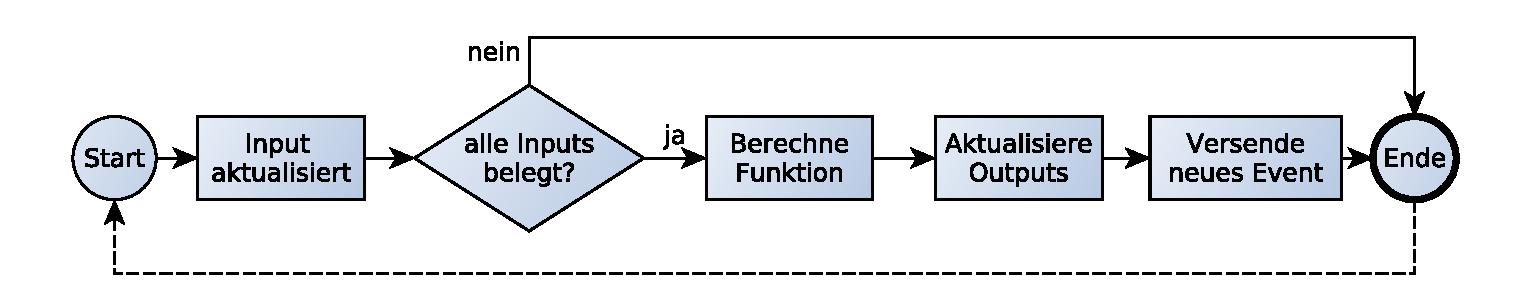
\includegraphics[width=1\textwidth]{bilder/chapter4/chapter4_2/funktionsblockablauf.pdf}
  \caption{Standardablauf innerhalb eines Funktionsknotens, wenn eine Input-Schnittstelle aktualisiert wird.}
  \label{fig:seqfunktionsblock}
\end{figure}
Wenn sich eine Input-Schnittstelle durch ein eintreffendes Ereignis aktualisiert wird, prüft der Transducer nach, ob sämtliche Input-Schnittstellen einen Wert besitzen. Der Knoten nimmt dann seine Transformation der Events vor, gibt das Ergebnis an die Output-Schnittstellen weiter, welche das neue Ereignis versenden. Folgendes ist hierbei zu beachten: 
\begin{itemize}
    \item Eingehende Signale werden nicht wie bei \ac{DBP} üblich, in der Input-Schnittstelle in einer \textit{Queue} gepuffert und nacheinander abgearbeitet, sondern überschrieben. Der Grund hierbei ist, dass cBlocks zu jeder Zeit auf den momentanen Zustand ihrer Umgebung reflektieren sollen. Es macht beispielsweise wenig Sinn, nicht mehr aktuelle Umgebungstemperaturen nacheinander abzuarbeiten.
    \item Events werden von Funktionsknoten nicht konsumiert. Aufgrund gleicher Überlegungen wie beim vorherigen Punkt, sollen die Events immer den momentanen Zustand der physischen Umgebung widerspiegeln, in der sich die (physischen) cBlocks befinden. Gibt es bspw. mehrere Sensoren mit unterschiedlichen Abtastfrequenzen müssen sämtliche Signale immer auf das Signal des Langsamsten warten. In solchen Fällen, wird das letzte Signal als das Aktuellste betrachtet und zur Durchführung der Funktion verwendet.
\end{itemize}
 Die Funktionen zur Transformation von Ereignissen, orientieren sich an den funktionalen Anforderungen \hyperref[tab:fanf]{FA\#1}  bis  \hyperref[tab:fanf]{FA\#6}:
 \begin{itemize} 
     \item Bei \textbf{Bool'schen Gattern} handelt es sich um logische Operationen, die auf ein oder mehrere bool'sche Signale angewandt werden. Zu den Funktionen zählen: Negation, logisches Und/Oder und exklusives Oder ($\neg, \land, \lor, \oplus$). Sie überprüfen den Ausdruck abhängig der Eingänge auf Wahrheit und geben das bool'sche Ergebnis weiter.
     \item Zu \textbf{Vergleichsoperationen} gehören sämtliche Operationen, die zwei Zahlen miteinander vergleichen können, und einen bool'schen Wert ausgeben ($<,\leq,=,\neq,\geq,>$).
     \item \textbf{Zeitgesteuerte Operationen} erlauben es dem Nutzer Signale auf ihre temporären Eigenschaften zu manipulieren d.h. Signale zeitlich zu verzögern oder Signale periodisch zu wiederholen.
     \item \textbf{Konvertierungsoperationen} wandeln Signale um, indem sie den Wertebereich des Eingangssignals auf einen vordefinierten Zielbereich des Ausgangssignals zuweisen. Dies kann auf zwei weisen geschehen: kontinuierliche Wertebereiche ($\left [ 1,2,3,...,n \right ] \rightarrow \left [ -n,...,-3,-2,-1 \right ]$) oder kategorische Wertebereiche ($\left [ \geq20, \leq30  \right ] \rightarrow \left [ kalt,heiss \right ]$)
     \item Der \textbf{Generische Operator} erlaubt es Experten ihre eigenen Transformationen in Programmcode zu beschreiben. Dieser Programmcode kann beliebig viele Ein- und Ausgänge besitzen sowie ein beliebige Kombination von Datentypen, solange sie mit denen von Tabelle \ref{tab:datentypenpayloads} übereinstimmen
 \end{itemize}
 Es können noch weitere vorgefertigte Funktionen definiert werden, allerdings würde dies den Rahmen dieser Arbeit hinausgehen und wäre nicht Zielführend, führ die Definition eines \ac{EUD}-Systems. Allerdings wird durch Funktionsknoten mit Nutzer-definierter Logik eine Schnittstelle vorgesehen, die es dem Endnutzer erlaubt, eigene Transformationslogik einzuprogrammieren. Somit wird dem Endnutzer erlaubt, flowws durch jede beliebige Funktion zu erweitern.
 
\subsubsection{3. Eventkonsumierung} \label{subsubsec:evebtkonsumierung}
Mit dem Konsumieren der Events schließt sich der Kreis, indem ein initiales physisches Phänomen, dass durch die Sensor-cBlocks aufgenommen wurde in einem neuen physischen Phänomen, dass vom Aktor-cBlock erzeugt wird (siehe Abbildung \ref{fig:beispielflowws}). 

Jeder Aktor-cBlock, der mit flowws verbunden wird, ist ähnlich wie bei den Sensor-cBlocks mit einer virtuellen Abbild (hier: Aktorknoten) repräsentiert. Ein Aktorknoten ist intern eine \ac{FSM} wie sie in Kapitel \ref{subsec:fsmprogrammierung} beschrieben. Hierbei werden vom Endnutzer Zustände, Übergänge und Übergangslogik definiert um dem Aktor ein gewünschtes Verhalten zu geben.

 \begin{figure}[h]
  \centering
  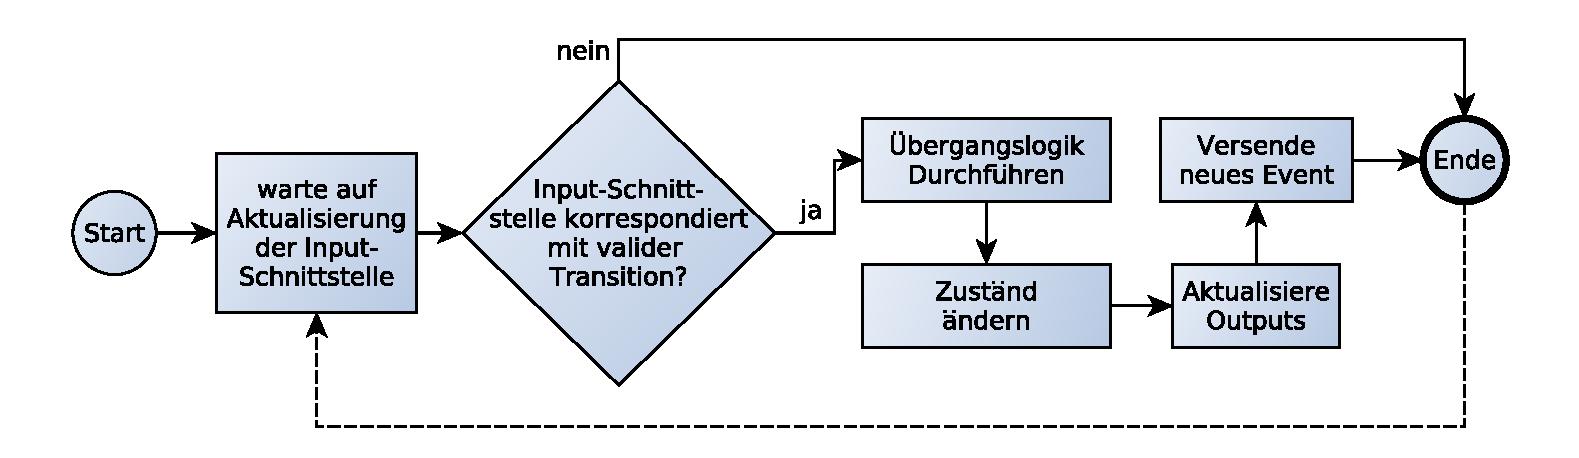
\includegraphics[width=1\textwidth]{bilder/chapter4/chapter4_2/aktorblockablauf.pdf}
  \caption{Standardablauf innerhalb eines Aktorknotens, wenn eine Input-Schnittstelle aktualisiert wird.}
  \label{fig:seqaktorblock}
\end{figure}

Jeder Aktorknoten besitzt zusätzlich zu seiner \ac{FSM} zwei weitere Komponenten:
\begin{itemize}
    \item \textbf{Aktoreigenschaften} sind alle Eigenschaften, welche die Art des physikalische Signals beeinflussen. Ein LED-cBlock kann die Aktoreneigenschaften \texttt{(r,g,b)} und \texttt{(Brightness)} besitzen; ein Lautsprecher-cBlock kann die Eigenschaften \texttt{(AudioFrequency)} und \texttt{(Volume)} besitzen oder ein LCD-cBlock kann die Eigenschaft \texttt{(DisplayText)} besitzen. Vorgegeben werden diese Eigenschaften von dem cBlocks \textit{Back-end}. Auf Hardwareebene werden solche Aktoreneigenschaften als \textbf{Ressource} bezeichnet. Von diesem abstrakten Begriff wird aufgrund von Benutzerfreundlichkeit allerdings in flowws Abstand genommen.
    \item \textbf{Aktorfunktionen} sind der einzige Weg innerhalb von flowws, Aktoreigenschaften direkt zu manipulieren. Jeder Aktorknoten wird mit einem Menge von Funktionen geliefert. Diese bestehen aus Funktionen wie \texttt{setColor()}, \texttt{setBrightness()}, \texttt{setFrequency()}, etc; und ermöglichen dem Endnutzer den Aktor durch geschickte Modellierung der Übergangslogik zu manipulieren. Anders als die Aktoreigenschaften besitzen Experten die Möglichkeit, zusätzliche Funktionen hinzufügen und somit die Flexibilität von Aktoren bei der Manipulation ihrer Eigenschaften erhöhen.
\end{itemize}

In Abbildung \ref{fig:seqaktorblock} ist der Ablauf zu sehen, der Durchgeführt wird, sobald ein neues Ereignis eintrifft. Zuerst ermittelt der Aktorknoten mit welchem Übergang die aktualisierte Input-Schnittstelle korrespondiert. Als Nächstes wird überprüft ob der Übergang erlaubt ist abhängig von dem Zustand, indem sich der Aktorknoten momentan befindet. Ist dies der Fall, wird die Übergangslogik ausgeführt und abhängig davon, des Events und der Aktorfunktionen die Eigenschaften des Aktors verändert. Durch die Veränderung der Aktoreigenschaften wird ein physikalisches Signal erzeugt. Ebenso kann ein neues Signal erzeugt werden und über eine Output-Schnittsstelle, welches ebenfalls mit der Übergangslogik korrespondiert, versendet werden. Ein Aktorknoten ist somit mehr als nur ein Konsument; er kann wie ein Sensorknoten neue Signale erzeugen, welche wiederum transformiert und von weiteren Aktorknotens konsumiert werden können.

\subsubsection{Zusammenfassung}
Hiermit wurde das Programmiermodell von flowws geklärt, eine Fusion von \ac{DBP} und \ac{FSM}. Es handelt sich hierbei um eine neues Programmiermodell, welches noch nicht innerhalb eines \ac{EUD}-Werkzeugs verwendet wurde. Aus diesem Grund, kann noch keine objektive Aussage über die Effektivität des Modells hinsichtlich Benutzerfreundlichkeit gemacht werden. Nichtsdestotrotz kann man die erhofften Vorteile logisch schlussfolgern:
\begin{itemize}
    \item \textbf{zu \hyperref[tab:NFA0]{NFA\#0} -- Sequentielle und Parallele Programmierung} Das Problem aus Kapitel \ref{sec:problemanalyse} wurde durch die Kombination von \ac{DBP} und \ac{FSM} beseitigt.
    \item \textbf{zu \hyperref[tab:NFA2]{NFA\#2} -- Leicht Erlernbar} Das Modell basiert auf \ac{DBP} und \ac{FSM}. Beides sind Konzepte die in der Informatik und Elektrotechnik weite Verbreitung finden. Diese Beliebtheit haben beide Konzepte ihrer Fähigkeit schwere Konzepte (Parallelität und \textit{State-Management}) intuitiv darzustellen zu verdanken. Zusätzlich sind Konzepte wie \ac{DBP} und \ac{FSM} auch in verschiedenen Werkzeugen die häufig von Designern verwendet werden (bspw. \textit{Game Engines} und 3d Modellierungs Software). Es besteht also eine gute Chance, dass auch nicht Experten die Konzepte von flowws schnell erlernen können.
    \item \textbf{zu \hyperref[tab:NFA2]{NFA\#2} -- Leichter Verständlich} \ac{DBP} und \ac{FSM} besitzten Pendants in der UML. Aus diesem Grund, lassen sich beide Teile gut graphisch Darstellen. Die bildliche Darstellung sollte eine bessere Verständlichkeit über die Vorgänge innerhalb des Programmes führen und somit etwaige Fehlersuche beschleunigen.
    \item \textbf{zu \hyperref[tab:NFA5]{NFA\#5} -- Flexibel} flowws bringt mit Funktionsknoten und Aktorfunktionen viel vorgefertigte Programmlogik mit. Allerdings können beide Elemente auch durch Experten erweitert werden um flowws optimal auf den Anwendungsfall anzupassen.
   
\end{itemize}

Im nächsten schritt wird die graphische Oberfläche und Darstellung der einzelnen Elemente sowie die Interaktionen mit ihnen geklärt.
\section{Graphisches Modell}\label{sec:graphischesmodell}
Im vorherigen Kapitel wurde das grundlegende Programmierungskonzept von flowws erklärt und anhand der Anforderungen gegenüber dem System sowie anhand der Probleme bestehender Systeme begründet. Wie allerdings schon in der Einleitung (Kapitel \ref{sec:einleitungkonzept}) geschrieben, benötigt die \ac{EUD} eine graphische Oberfläche, mit welcher der Endnutzer interagieren kann. Entscheidungen anhand von Anforderungen, Probleme und \ac{CD} rationalisiert.
 
\subsection{Design Richtlinien}
Für die graphische Oberfläche von flowws müssen die einzelnen Elemente, die im vorherigen Kapitel beschrieben wurden, durch eine graphischen Repräsentant abgebildet werden. Der Endnutzer muss mit diesen Abbildungen interagieren, um die gewünschte Betriebsverhalten des Gesamtsystems zu erreichen. Um eine kohärente \ac{UX} zu erreichen, sollen Abbildung und Interaktion einer geteilten Philosophie unterliegen; einem Satz von Regeln, der die Design-Entscheidungen rationalisiert und sich an den Rahmenbedingungen des Projekts orientiert.

\paragraph{Nähe zur Realität}\label{par:naehezurrealitaet} Es sollte immer bedacht werden, dass die (physischen) cBlocks zu jedem Zeitpunkt des Design Prozesses verwendet werden. Graphisch soll diese physische Bindung reflektiert werden. Aus diesem Grund soll die visuelle Darstellung und die Interaktionen der \ac{EUD} wenn möglich Bezug zu den cBlocks oder zumindest mit der Domäne der \ac{IoT} und Elektrotechnik besitzen. Es wird sich dadurch erhofft, dass \textbf{Domänennähe} und \textbf{funktionale Aussagekraft} (siehe Tabelle \ref{tab:cognitivedimensions}) zu erhöhen und somit die Anforderungen \hyperref[tab:NFA2]{NFA\#2} und  \hyperref[tab:NFA3]{NFA\#3} zu lösen.

\paragraph{Fokus bewahren}\label{par:fokusbewahren} Design ist ein kreativer Prozess von dem flowws nicht durch seine eigene Komplexität ablenken soll. Um schnell und zielführend Arbeiten zu können, soll flowws Vorgaben machen an denen sich der Endnutzer orientieren kann. Durch graphische Signale wie Farben und Formen, soll dem Nutzer das Rätseln über die Rolle einzelner Komponenten erspart werden.

\paragraph{Fehler vorbeugen}\label{par:fehlervorbeugen} Statt zeitaufwändige Fehlersuche zu unterstützen ist es sinnvoller, Fehler durch graphische Hinweise im Vorfeld zu vermeiden (siehe Tabelle \ref{tab:cognitivedimensions} und  \hyperref[tab:NFA4]{NFA\#4}).

\paragraph{'\textit{'Move fast and break things}''}\label{par:movefast} Prototyping ist schnell und explorativ. Deswegen soll die \ac{GUI} von flowws diese schnelle Art von Arbeit durch bspw. Austauschbarkeit der Komponenten unterstützen.

\paragraph{''\textit{Grow-As-You-Go}''}\label{par:growasyougo} flowws ist kein Lehrwerkzeug sondern soll produktives Arbeiten ermöglichen. Die technischen Fähigkeiten der Endnutzer sind allerdings sehr Variabel. Zusätzlich ist zu erwarten, dass das technische Verständnis mit der stetigen Benutzung des Werkzeugs wächst. Daher soll der Funktionsumfang der Oberfläche mit den Fähigkeiten des Endnutzers wachsen können. Das Erlernen der Oberfläche durch nützliche Hinweise unterstützen (siehe \hyperref[tab:NFA2]{NFA\#2}). Gleichzeitig aber soll sie nicht obsolet werden, bei komplexeren Szenarien, in denen spezifischere Funktionalität abverlangt wird (siehe  \hyperref[tab:NFA5]{NFA\#5}).

%%%%%%%%%%%%%%%%%%%%%%%%%%%%%%%%%%%%%%%%%%%%%%%%%%%%%%%%%%%%%%%%%%%%%%%%

\subsection{Workspace}
\begin{figure}[h]
  \centering
  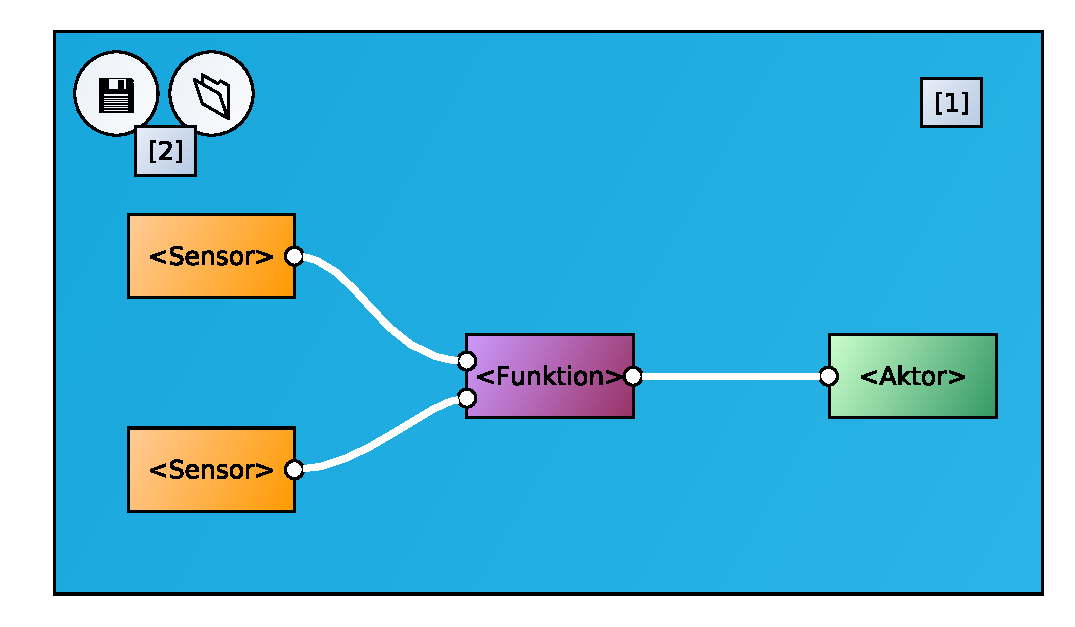
\includegraphics[width=.75\textwidth]{bilder/chapter4/chapter4_3/workspace.pdf}
  \caption{[1] ist der Workspace mit einem generischen Graph. [2] sind Funktionen, die es erlauben die Graphen zu verwalten.}
  \label{fig:workspace}
\end{figure}


\paragraph{Kurzbeschreibung} Der Workspace (dt. ''Arbeitsbereich'') ist die primäre Komponente von flowws. Innerhalb dieser Komponente werden flowws-Graphen bzw. flowws-Programme erstellt, organisiert, administriert und auf Fehler untersucht. Er dient als digitale Leinwand für den Designer, um im Zusammenspiel mit den physischen cBlocks Prototypen zu erstellen.

\paragraph{Rahmenbedingungen \& Entscheidungen} Der digitale Arbeitsbereich, soll den physischen Arbeitsbereich nachbilden. flowws wird immer simultan zu cBlocks verwendet, d.h. der Endnutzer manipuliert und interagiert während des gesamten Entwicklungszyklus mit den cBlocks. Aus diesem Grund, arbeitet der Endnutzer zu jederzeit an maximal einem Graphen. Dies steht im Kontrast zur Programmierung in \acp{IDE}, in denen an mehreren Projekten simultan gearbeitet werden kann und somit ein hoher Grad von Kontextwechsel benötigt wird. Bei flowws soll sich der Designer ähnlich wie bei einer Leinwand vollständig auf die Erstellung des Graphen konzentrieren können, ohne sich mit einer Kakophonie von Icons und Untermenüs auseinandersetzen zu müssen. 

\textbf{Aktionen}, die von und in dieser Komponente durchgeführt werden können: 
\begin{itemize}
    \item \textbf{Anzeigen von Knoten} Der Workspace dient dem Anzeigen von Sensor-, Aktor- und Funktionsknoten. 
    \item \textbf{Administration von Graphen} Der Graph kann über den Workspace gespeichert, geladen und verwaltet werden. 
\end{itemize}

\paragraph{Darstellung} Der Workspace bewusst schlicht gehalten, wie in Abbildung \ref{fig:workspace} gezeigt wird. Bis auf zwei Knöpfe zum Laden und Speichern von Graphen sind keine weiteren Interaktionsmöglichkeiten zu sehen. Diese Entscheidung wurde bewusst so getroffen. Der leere Workspace soll einen leeren Schreibtisch nachahmen (siehe ''Nähe zur Realität''). Aus diesem Grund, werden Sensorknoten und Aktorknoten automatisch angezeigt, wenn ihre physischen Gegenstücke mit dem System verbunden sind. Die Schreibtisch-Metapher soll unterstützt werden, indem die Optik des Workspace an eine typische Schneideunterlage, wie sie in Werkstätten zu finden ist, angelehnt.

%%%%%%%%%%%%%%%%%%%%%%%%%%%%%%%%%%%%%%%%%%%%%%%%%%%%%%%%%%%%%%%%%%%%%%%%

\subsection{flowws-Graph}
\subsubsection{Knoten}
\begin{figure}[h]
  \centering
  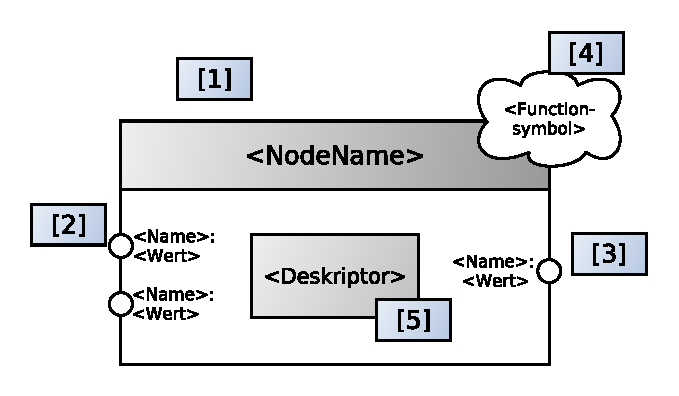
\includegraphics[width=.8\textwidth]{bilder/chapter4/chapter4_3/genericnode.pdf}
  \caption{Ein generischer Knoten.}
  \label{fig:genericnode}
\end{figure}

\paragraph{Kurzbeschreibung} Knoten sind die fundamentalen Bausteine eines jeden flowws-Graphen. Sie erzeugen, transformieren und konsumieren Daten auf die Weise, auf die sie vom Endnutzer kompositioniert und konfiguriert sind. Alle Knoten (Sensoren, Funktionen, Aktoren) teilen fundamentale Charakteristiken (Identität, Form), Subkomponenten (Input-/Output-Schnittstellen, Deskriptor) und Interaktionen (Anordnen, Erstellen, Löschen) miteinander. 

\paragraph{Rahmenbedingungen \& Entscheidungen} Jeder Block muss eindeutig von seinem Typus identifizierbar und seinem physischen Pendant zuordenbar sein. Da es viele Arten von Knoten gibt, muss es möglichst leicht erkenntlich sein, welche Funktion er übernimmt, welche Daten ein- und ausfließen und aus welchem Grund der Block seine Entscheidung getroffen hat.

\textbf{Aktionen}, die von und in dieser Komponente durchgeführt werden können: 
\begin{itemize}
    \item \textbf{Anordnen} Die Knoten lassen sich hinsichtlich ihrer Position organisieren bzw. anordnen. Dadurch kann der Endnutzer die Position der physischen Aktoren/Sensoren mit denen der Virtuellen abgleichen (siehe ''Nähe zur Realität'').
    \item \textbf{Verbindung starten/enden} Die Schnittstellen dienen als Interaktionspunkte um Verbindungen zu starten und zu enden.
    \item \textbf{Deskriptor ändern} Durch das ändern des Deskriptors kann das Verhalten von Knoten auf Eingangssignale konfiguriert werden.
\end{itemize}

\paragraph{Darstellung} Der in Abbildung \ref{fig:genericnode} dargestellte generische Block besitzt alle Merkmale, die in Aktor-,Sensor- und Funktionsknoten vorhanden sind. Die quadratische Darstellung des Knoten wurde einer komplexeren Darstellung bevorzugt, um eine visuelle Nähe zum Quader-Design der cBlocks zu erreichen (siehe Abbildung \ref{fig:cblockfoto}). \textbf{[1]} ist die Identifikationsleiste des Blocks. Sie gibt durch Farbe Aufschluss über den Typ (\colorbox{sensororange}{Sensor}, \colorbox{aktorgreen}{Aktor} und \colorbox{funcviolet}{Funktion}) und durch Text Aufschluss über die Rolle (z.B. ''Logisches-Gatter'') des Knotens. \textbf{[2]} und \textbf{[3]} sind die Input- und Output Schnittstellen. Sie dienen als Anfangs- und Endpunkte für Verbindungen, besitzen Namen durch die sie Unterscheidbar werden (''OperandA'' etc.) und zeigen den letzten Wert an, der über die Schnittstelle empfangen bzw. versendet wurde (siehe \hyperref[tab:NFA1]{NFA\#1}). \textbf{[4]} ist der Knoten-Indikator und gibt wie \textbf{[2]} Aufschluss über den Knotentyp und Knotenrolle. Er zeigt zum einen durch seine Form den Typ und zum Anderen mit einem Symbol die konkrete Rolle des Knotens (bspw. Sensorknoten: Temperatur, Funktionsknoten: Logisches-Gatter, etc.) an. \textbf{[5]} ist der Knoten-Deskriptor. Er gibt Endnutzer Aufschluss, welche konkrete Instruktion (bspw. logisches Und) auf den Eingabedaten ausgeführt werden bzw. in welchem Zustand sich der Knoten momentan befindet, wenn es sich um einen Aktorknoten handelt.

%%%%%%%%%%%%%%%%%%%%%%%%%%%%%%%%%%%%%%%%%%%%%%%%%%%%%%%%%%%%%%%%%%%%%%%%

\subsubsection{Verbindungen/Kanten}
\begin{figure}[h]
  \centering
  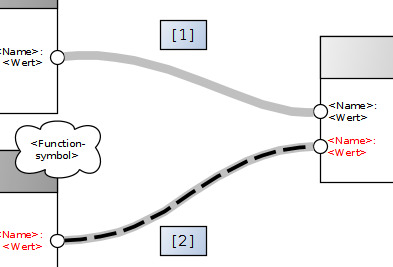
\includegraphics[width=.6\textwidth]{bilder/chapter4/chapter4_3/links.png}
  \caption{Zwei Kanten verbinden vier Input-/Output-Schnittstellen. [1] ist inaktiv während über [2] ein Signal übertragen wird. Man beachte die kurzzeitige Färbung der Input-/Output-Schnittstellen, die auf eine Aktualisierung des Wertes hinweisen.}
  \label{fig:genericlink}
\end{figure}


\paragraph{Kurzbeschreibung} Verbindungen/Kanten sind die Transportwege der Daten, zwischen den einzelnen Knoten. Ähnlich wie ein Leitungen auf einer Platine stellen eine Kante den Transportweg der Signale von einer Output-Schnittstelle zu einer Input-Schnittstelle dar.

\paragraph{Rahmenbedingungen \& Entscheidungen} Jede Verbindung stellt eine eins-zu-eins Beziehung zwischen zwei Schnittstellen dar. Dabei muss sichergestellt werden, dass nur Schnittstellen mit kompatiblen Datentypen verbunden werden können (siehe \hyperref[tab:NFA4]{NFA\#4}). 

\textbf{Aktionen}, die von und in dieser Komponente durchgeführt werden können: 
\begin{itemize}
    \item \textbf{Erstellen} Durch betätigen einer Output-Schnittstelle wird der Erstellungprozess einer Verbindung gestartet und endet mit dem Betätigen einer kompatiblen Input-Schnittstelle oder dem Erstellen eines kompatiblen Funktionsknotens.
    \item \textbf{Löschen} Löscht die Datenübertragung zwischen zwei Schnittstellen und bereinigt die Input-Schnittstelle, in der die Verbindung versinkt.
\end{itemize}

\paragraph{Darstellung} Die Darstellung einer Verbindung ist eine Bézierkurve, die an einer Input-Schnittstelle entsteht und an einer Output-Schnittstelle endet (Abbildung \ref{fig:genericlink}). Sobald Daten durch eine Verbindung fließen, wird eine kurze Animation innerhalb der Bézierkurve gespielt, die den Transfer von Daten entlang der Flußrichtung darstellt (\textbf{[2]}). Der Datentransfer geht verzögerungsfrei vonstatten, ähnlich wie der Transfer von elektrischen Signalen durch Kabel. Deswegen wird die Animation über die ganze Länge der Kurve kurzlebig dargestellt (siehe ''Nähe zur Realität'').

%%%%%%%%%%%%%%%%%%%%%%%%%%%%%%%%%%%%%%%%%%%%%%%%%%%%%%%%%%%%%%%%%%%%%%%%%%%%%%%%%%%%%%%%%%%%%%%%%%%%%%%%%%%%%%%%%%%%%%%%%%

\subsubsection{Sensorknoten}
\begin{figure}[h]
\centering
\begin{subfigure}{.5\textwidth}
  \centering
  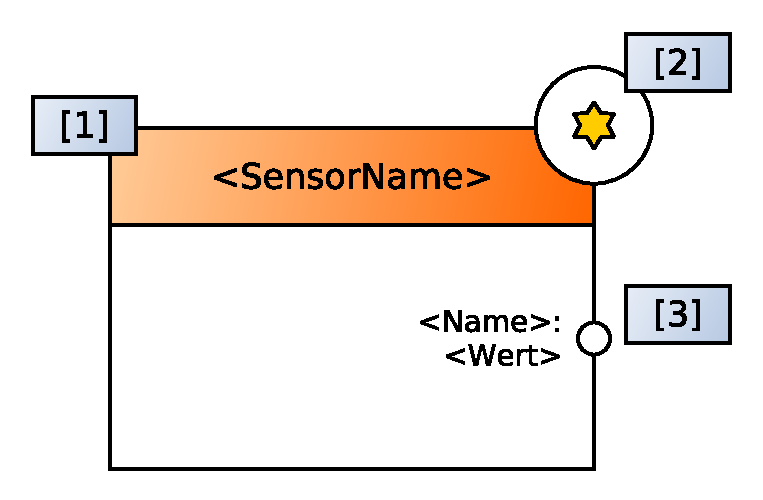
\includegraphics[width=1\linewidth]{bilder/chapter4/chapter4_3/genericsensornode.pdf}
  \caption{}
  \label{fig:genericsensornode}
\end{subfigure}%
\begin{subfigure}{.5\textwidth}
  \centering
  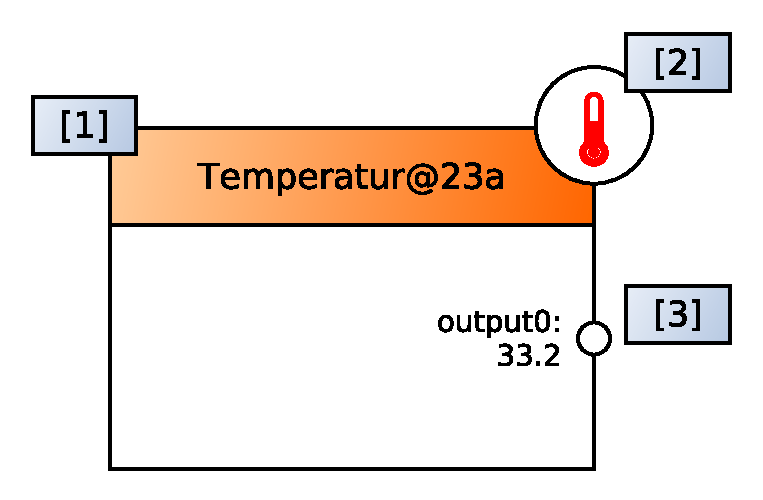
\includegraphics[width=1\linewidth]{bilder/chapter4/chapter4_3/instancesensornode.pdf}
  \caption{}
  \label{fig:sensornodetemperature}
\end{subfigure}
    \caption{Generischer Sensorknoten (a) und Temperatur-Sensorknoten (b)}
    \label{fig:sensornodes}
\end{figure}

\paragraph{Kurzbeschreibung}  Sensorknoten sind die virtuellen Gegenstücke zu den Sensor-cBlocks. Jeder Sensorknoten erzeugt Ereignisse, sobald der Sensor-cBlock eine neue Stichprobe in der Realität entnimmt. Alle Ereignisse werden mit einem Datentyp und dem Messwert als \textit{Payload} über die Output-Schnittstelle an nachfolgende Knoten verteilt. Sobald ein Sensorknoten existiert, sendet er stetig Daten und erlaubt dem Endnutzer kontinuierlich das Verhalten des Graphen zu überprüfen (siehe ''Fehler vorbeugen'' bzw. \hyperref[tab:cognitivedimensions]{fortwährende Evaluation}).

\paragraph{Rahmenbedingungen \& Entscheidungen} Einzelne Sensor-cBlocks können mehrere verschiedene Messwerte auslesen (bspw. Temperatur und Luftfeuchtigkeit im selben Sensor-cBlock). Dem Sensorknoten muss es möglich sein, diese Multifunktionalität abbilden zu können. Es kann sein, dass mehrere Sensor-cBlocks von der gleichen Sorte im selben Prototypen verwendet werden. In diesem Fall, muss es für den Endnutzer möglich sein, die Sensorknoten klar unterscheiden zu können. Gleichzeitig muss es dem es möglich sein leicht, das  physikalische Pendant zu einem virtuellen Sensorknoten zu identifizieren. Ein weiterer Punkt ist die Abtastfrequenz. Sensor-cBlocks liefern Daten in kurz-, lang- oder aperiodischen Frequenzen. Sensorknoten müssen aus diesem Grund darauf achten, synchron mit ihrem physischen Gegenstück, Ereignisse zu erzeugen. Sensorknoten können weder erstellt noch gelöscht werden. Der Status des Sensorknotens, also auch seine Existenz, ist an den Status des Sensor-cBlocks gebunden.

\textbf{Aktionen}, die von und in dieser Komponente durchgeführt werden können: 
\begin{itemize}
    \item \textbf{Identifizieren} durch Betätigen des Knoten-Indikators blinkt die Status LED des korrespondierenden cBlocks. Somit lässt sich sein physisches Pendant identifizieren (siehe ''Nähe zur Realität'').
\end{itemize}

\paragraph{Darstellung} In Abbildung \ref{fig:sensornodes} ist ein generischer Sensorknoten (a) und ein konkreter Temperatur-Sensorknoten (b) dargestellt. Jeder Sensorknoten ist durch eine eindeutige Adresse in der Titelleiste [1] voneinander unterscheidbar. Simultan wird durch \textbf{[2]} der Knotentyp ($\bigcirc$) und seine Rolle ($Thermometer \rightarrow Temperatur$) preisgegeben. \textbf{[3]} sind die Output-Schnittstellen. Jede Art von Messwert eines Sensor-cBlocks erhält einen separaten Output, der den aktuellen Messwert visualisiert. 

%%%%%%%%%%%%%%%%%%%%%%%%%%%%%%%%%%%%%%%%%%%%%%%%%%%%%%%%%%%%%%%%%%%%%%%%%%%%%%%%%%%%%%%%%%%%%%%%%%%%%%%%%%%%%%%%%%%%%%%%%%

\subsubsection{Funktionsknoten}
\begin{figure}[h]
\centering
\begin{subfigure}{.5\textwidth}
  \centering
  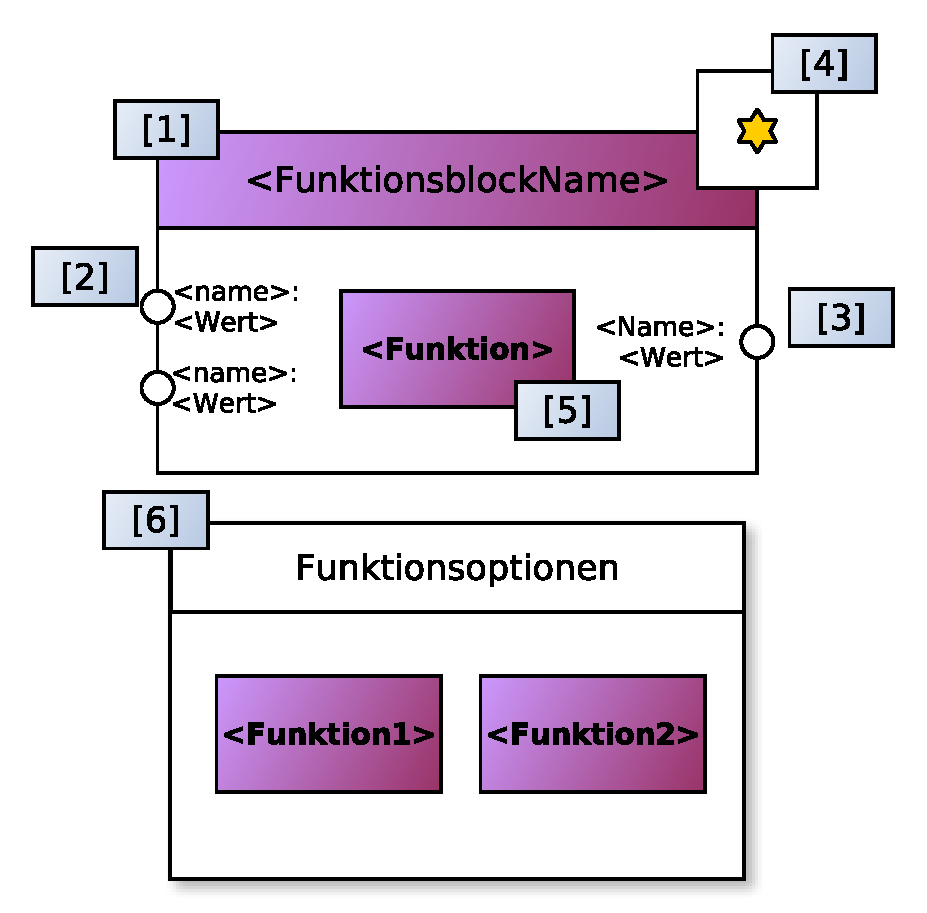
\includegraphics[width=1\linewidth]{bilder/chapter4/chapter4_3/genericfunctionnode.pdf}
  \caption{}
  \label{fig:functionnodesgen}
\end{subfigure}%
\begin{subfigure}{.5\textwidth}
  \centering
  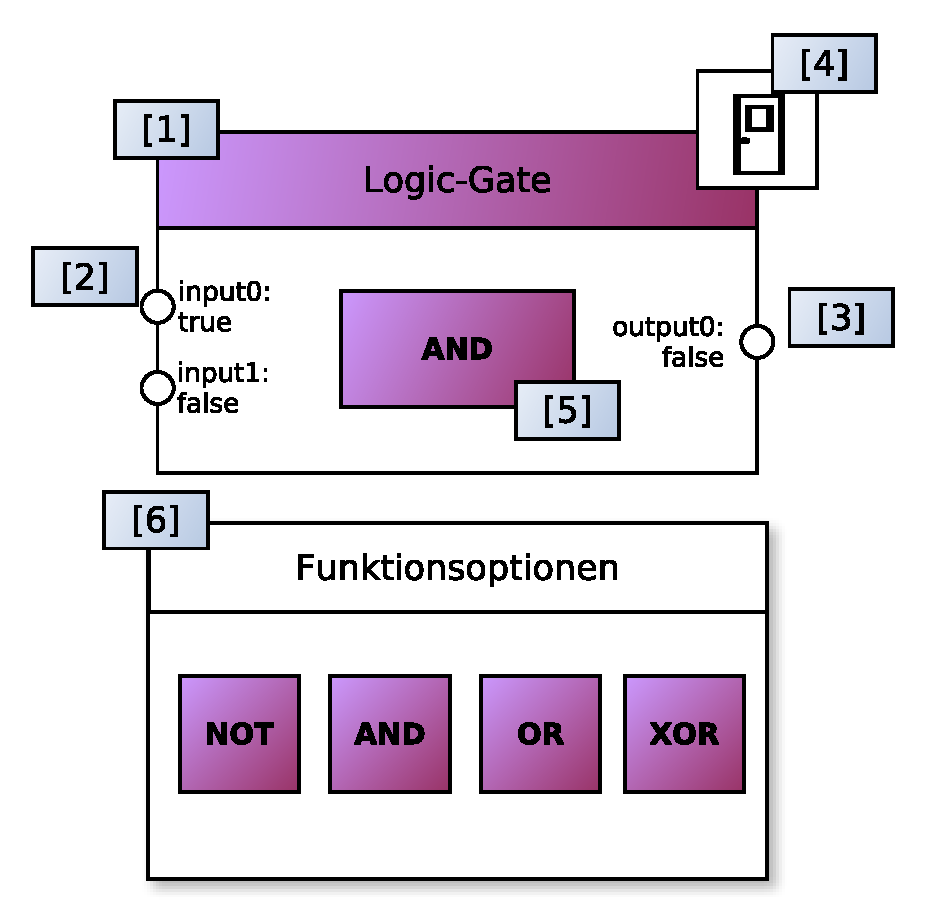
\includegraphics[width=1\linewidth]{bilder/chapter4/chapter4_3/instancegatefunctionnode.pdf}
  \caption{}
  \label{fig:functionnodesgate}
\end{subfigure}
    \caption{Generischer Funktionsknoten (a) und spezifischer Funktionsknoten ''Logisches-Gatter'' (b). Weitere Beispiele für Funktionsknoten im Anhang \ref{anhang:funktionsknoten}}
    \label{fig:functionnodes}
\end{figure}

\paragraph{Kurzbeschreibung} Funktionsknoten sind die Recheneinheiten des Graphen. Der Endnutzer benutzt sie um Signale zu kombinieren und aufzuwerten. Funktionsknoten kommen in einer Bandbreite von Operationsklassen (Logisches-Gatter, Vergleichsoperation, etc.), welche sich an den Datentypen der Ereignisse orientieren (\texttt{String}, \texttt{Number} und \texttt{Boolean}). Jede Operationsart besitzt eine Familie von entsprechenden Operatoren ($\neg, \land,\neq,\geq,$ etc.).

\paragraph{Rahmenbedingungen \& Entscheidungen} Es wurde sich dafür entschieden, Operatoren in Operationsklassen zu bündeln, statt jeder Operation in einen separaten Funktionsknoten auszulagern. Dies soll der Übersicht beitragen und somit das Prototyping beschleunigen (siehe \hyperref[par:movefast]{''Move fast...''}). Des Weiteren lässt sich dadurch die Funktion austauschen ohne den Knoten und somit die Verbindungen austauschen zu müssen (siehe ''vorzeitige Festlegung'' in Tabelle \ref{tab:cognitivedimensions}). Dies beschleunigt das Experimentieren mit verschiedenen Operatoren. Funktionsknoten sind rein virtuell und generisch. Sprich: anders als bei Sensoren/Aktoren können zwei komplett identische Knoten im gleichen Graph existieren.

Die \textbf{Aktionen}, die von und in dieser Komponente durchgeführt werden können: 
\begin{itemize}
    \item \textbf{Löschen} Funktionsknoten begründen ihre Existenz nicht auf ein physisches Pendant, deshalb sind sie anders als Sensor-/Aktorknoten löschbar.
    \item \textbf{Konfigurieren} Die konkrete Funktion wird durch Interagieren mit dem Deskriptor gewählt (siehe Abbildung \ref{fig:functionnodes} und Anhang \ref{anhang:funktionsknoten} für weitere Beispiele)
\end{itemize}

\paragraph{Darstellung}  Der Deskriptor \textbf{[5]} ermöglicht es den momentanen Operator auszulesen. Durch betätigen von [5] wird ein \textit{Modal} \textbf{[6]} geöffnet, indem sich der Operator konfigurieren lässt. In Abbildung \ref{fig:functionnodesgate} ist als Beispiel ein Logikgatter-Funktionsknoten dargestellt. Hier kann der Nutzer die verschiedenen bool'schen Operatoren im laufenden Betrieb konfigurieren und somit das Verhalten des gesamten Graphen zu Laufzeit ändern (siehe '' Move fast...''). Die Schnittstellen \textbf{[2]} und \textbf{[3]} erlauben Parameter und Ergebnis zur Laufzeit auszulesen und Fehler zu überprüfen.

%%%%%%%%%%%%%%%%%%%%%%%%%%%%%%%%%%%%%%%%%%%%%%%%%%%%%%%%%%%%%%%%%%%%%%%%%%%%%%%%%%%%%%%%%%%%%%%%%%%%%%%%%%%%%%%%%%%%%%%%%%

\subsubsection{Aktorknoten}

\begin{figure}[h]
\centering
\begin{subfigure}{.55\textwidth}
  \centering
  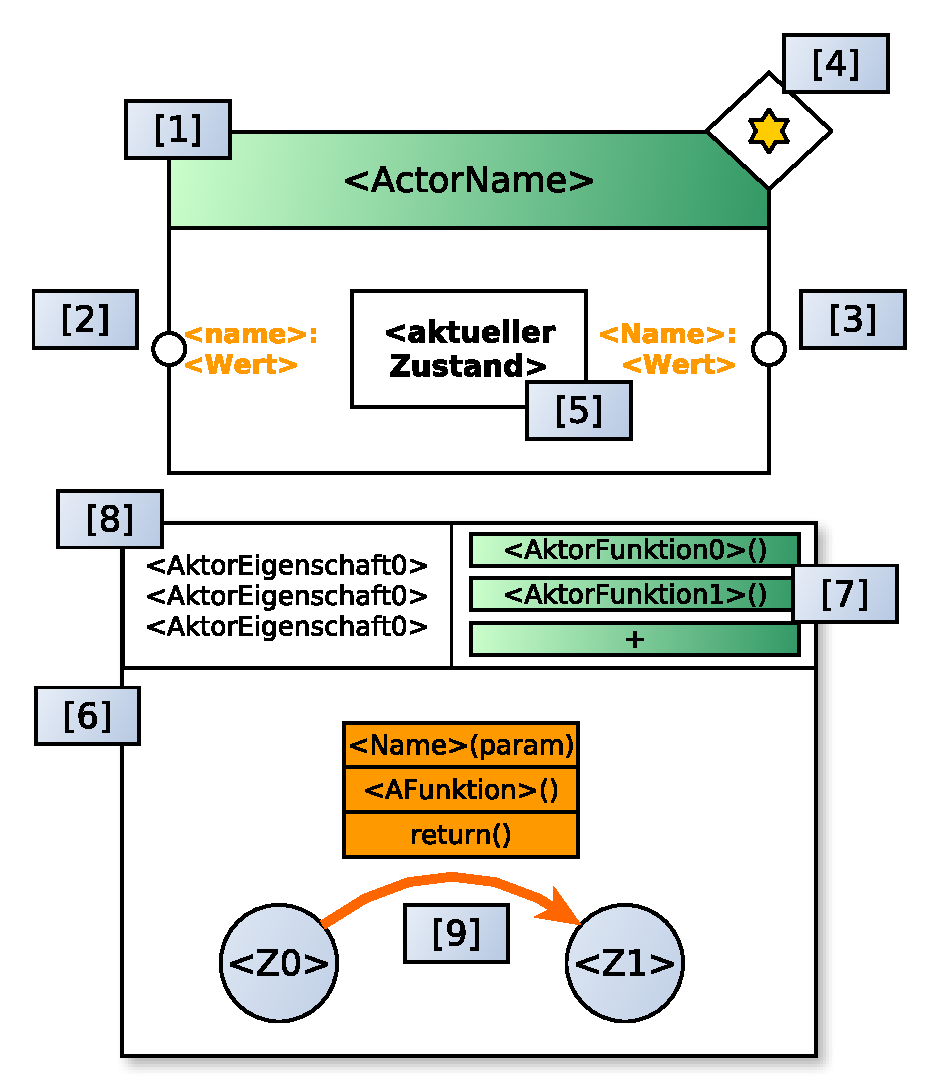
\includegraphics[width=1\linewidth]{bilder/chapter4/chapter4_3/genericactornode.pdf}
  \caption{}
  \label{fig:actorgeneric}
\end{subfigure}%
\begin{subfigure}{.55\textwidth}
  \centering
  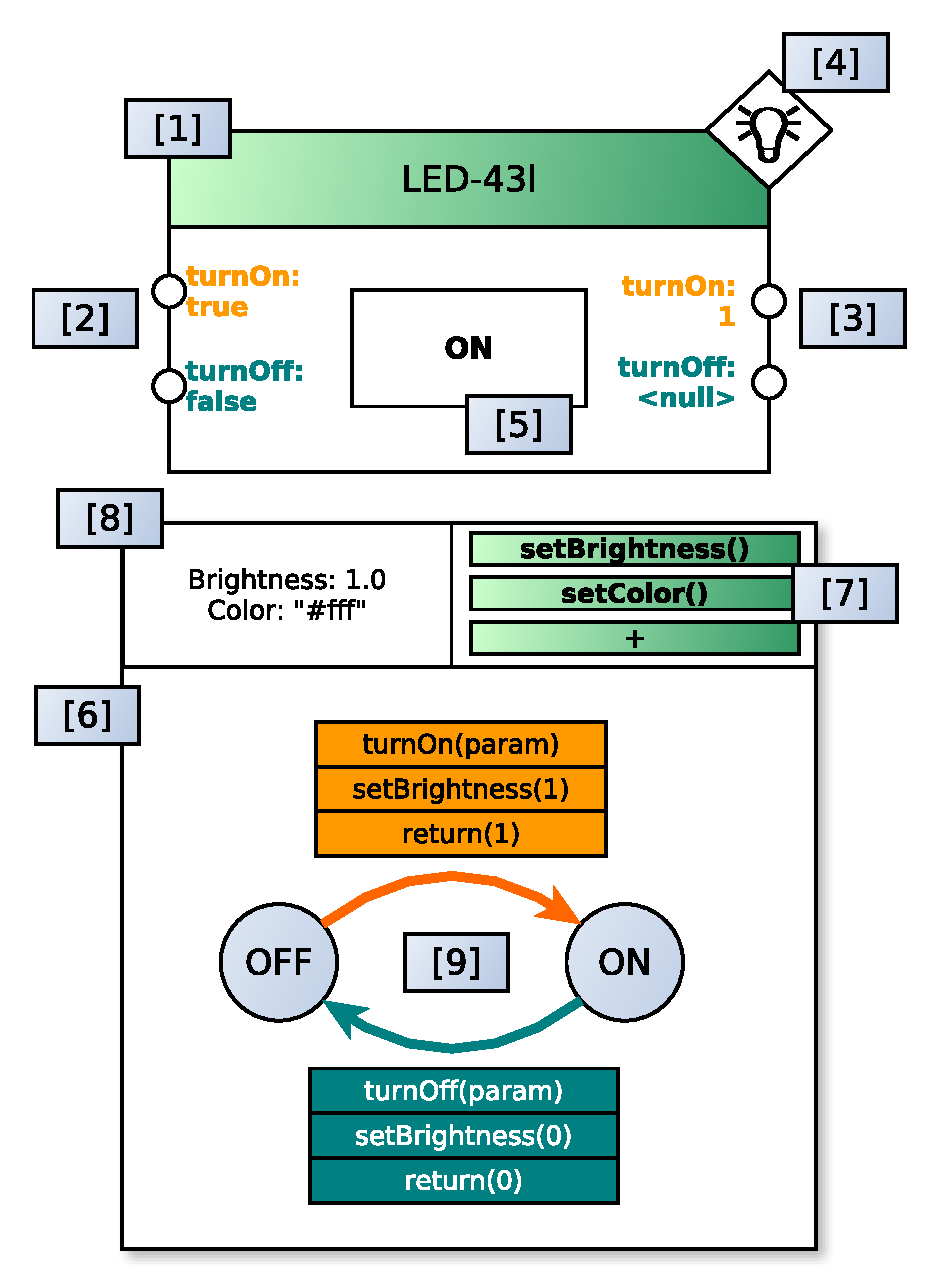
\includegraphics[width=1\linewidth]{bilder/chapter4/chapter4_3/instanceLEDactornode.pdf}
  \caption{}
  \label{fig:actorled}
\end{subfigure}
    \caption{Generischer Aktorblock (a) und spezifischer LED-Aktorblock (b)}
    \label{fig:actornodes}
\end{figure}


\paragraph{Kurzbeschreibung} Aktorknoten sind Sensorknoten ähnlich, indem auch sie, physikalisches Pendants in Form von Aktor-cBlocks besitzen. Durch das Einwirken von Ereignissen verändern Aktorknoten ihren Zustand und steuern somit Aktor-cBlocks. Die Steuerung wird vorgenommen durch eine, vom Endnutzer definierte, \ac{FSM}. Diese \ac{FSM} (siehe Abbildung \ref{fig:actorled} [6]) erlaubt es durch Aktorfunktionen (bspw. \texttt{setColor()}), Aktoreigenschaften (bspw. \texttt{color}) zu verändern und somit die physikalischen Signale des Aktor-cBlocks zu manipulieren. Aktorknoten sind neben dem eigentlichen Graphen die zweite programmierbare Komponente in flowws. Jeder Aktorknoten besitzt eine eingeschränkte Menge von Eigenschaften, die direkt mit den physikalischen Eigenschaften des Aktor-cBlocks korrespondieren. Ein Minimum von Aktorfunktionen wird von flowws vorgegeben.

\paragraph{Rahmenbedingungen \& Entscheidungen} Endbenutzern, denen die mitgelieferten Aktorfunktionen nicht ausreichen, soll es ermöglicht werden, diese nach belieben zu erweitern (siehe ''Grow as you go''). Des Weiteren soll Nutzern es möglich sein, mit den selben Interaktionen, mit denen der Graph modelliert wird, auch die \ac{FSM} zu programmieren (siehe \hyperref[par:fokusbewahren]{''Fokus bewahren''}). Dem Nutzer soll zu jedem Zeitpunkt möglich sein, das Verhalten des Aktors vorauszusagen und nachvollziehen zu können. Aktoren sollen ihren Zustand dem Rest des Graphen mitteilen zu können. Deshalb soll es der Endnutzer in der Lage sein, synthetische Signale zu definieren, die bei einem Zustandswechsel erzeugt werden. Der Status des Aktorknotens ist den Aktor-cBlock gebunden (siehe \hyperref[par:naehezurrealitaet]{''Nähe zur Realität''}). 

\textbf{Aktionen}, die von und in dieser Komponente durchgeführt werden können: 
\begin{itemize}
    \item \textbf{\ac{FSM} erstellen} Zustände, Übergänge und Übergangsfunktionen werden mithilfe der Aktorfunktionen und Aktoreigenschaften vom Endnutzer modelliert
    \item \textbf{Umfang der Aktorfunktionen erweitern} Um den Funktionsumfang zu erweitern können zustandslose Funktionen, welche Aktoreigenschaften modifizieren, vom Endnutzer in Programmcode spezifiziert werden.
\end{itemize}

\paragraph{Darstellung} Der Aktorknoten wird ähnlich wie der Funktionsknoten auf zwei Ebenen dargestellt: der Graphen-Ebene [1] und in Detail-Ebene [8]. Input- [2] und Output-Schnittstellen [3] korrespondieren bei Aktorknoten farblich und namentlich mit den Zustandsübergängen [9] um die Sichtbarkeit des Verhaltens auch außerhalb der Detailansicht zu garantieren (siehe ''Sichtbarkeit'' in Tabelle \ref{tab:cognitivedimensions}). Die momentane Ausprägung der Aktoreigenschaften wird in [8] dargestellt. Die verfügbaren Aktorfunktionen sind in [7] inspizierbar. Die Darstellung der \ac{FSM} in [9] besteht aus Ovalen die Zustände symbolisieren und farbigen Pfeilen die Übergänge definieren. Die Überganglogik wird in einer dreigeteilten Box dargestellt, die sich in Deklaration (Name korrespondiert mit [2] und [3]), Logik (Aktorfunktionen) und Rückgabewert (Der \textit{Payload} des vom Aktor erzeugten Events) aufteilt. Zur Laufzeit ist der momentane Zustand des Aktorknotens ist im Deskriptor [5] ersichtlich.

\subsubsection{Radialmenü}

\begin{figure}[h]
  \centering
  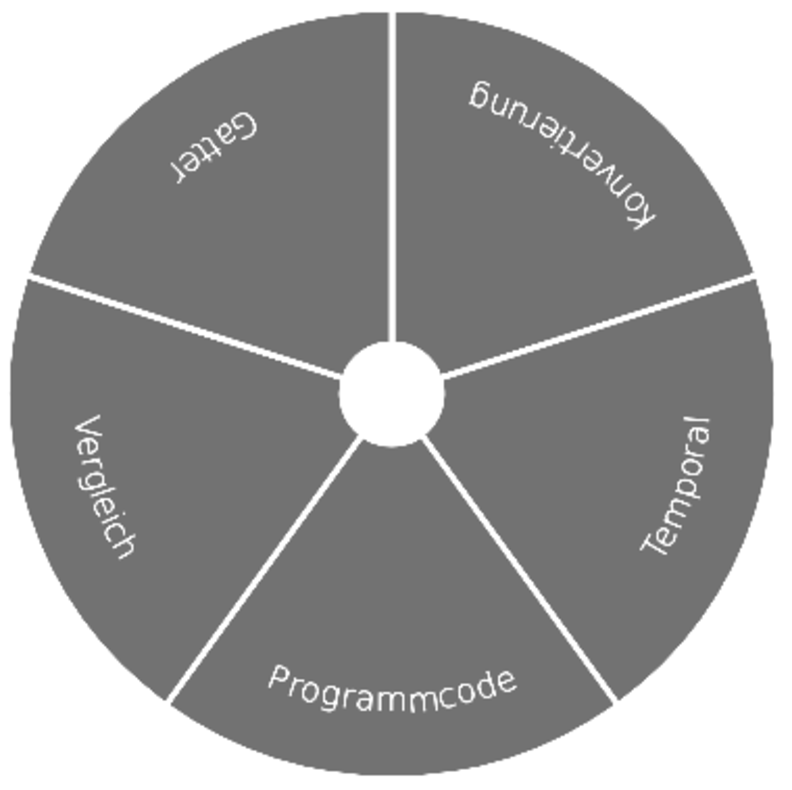
\includegraphics[width=.4\textwidth]{bilder/chapter4/chapter4_3/radialmenu.pdf}
  \caption{Das Radialmenu mit den fünf verschiedenen Operationsklassen aus Kapitel \ref{subsubsec:eventtrans} zur Auswahl}
  \label{fig:radialmenu}
\end{figure}

\paragraph{Kurzbeschreibung} Das Radialmenü ist ein Untermenü, das zu jeder Zeit auf dem Workspace aufgerufen werden kann. Es wird vom Endnutzer verwendet, um Funktionsknoten zu erzeugen.

\paragraph{Rahmenbedingungen \& Entscheidungen} Es wurde sich für ein Radialmenü entschieden, da es im Vergleich zu linearen Menüs schneller zu benutzen ist (siehe ''Move fast...'). Vor allem bei einer vergleichsweise geringen Anzahl von Optionen, die oft verwendet werden müssen (was bei flowws der Fall ist) sind laut \cite{kurtenbach1994user} Radialmenüs besonders effektiv. Das Menü ist kontextsensitiv, d.h. es soll immer nur Operationsklassen von Funktionsknoten zeigen, die zu jenem Zeitpunkt relevant sind. Dies soll zum einen, die Auswahl von inkompatiblen Funktionsknoten verhindern (siehe ''Fehler vorbeugen'') und zum anderen, durch das Verstecken unnötiger Informationen die Arbeitsgeschwindigkeit erhöhen (siehe ''Move fast...'').

Die \textbf{Aktionen}, die von und in dieser Komponente durchgeführt werden können: 
\begin{itemize}
    \item \textbf{Funktionsknoten erstellen} Das Radialmenü ist der einzige Weg für den Nutzer Funktionsknoten zu erstellen. Dazu ruft der Endnutzer das Radialmenü auf und wählt den gewünschten Operationsklassen von Funktionsknoten aus.
\end{itemize}

\paragraph{Darstellung} Das Radialmenü (Abbildung \ref{fig:radialmenu}) ist in fünf Segmente aufgeteilt, bei dem jedes Segment eine Art von Funktionsknoten repräsentiert. Das Radialmenü wird nur nach explizitem Aufruf durch den Endnutzer oder im Kontext von Interaktionen dargestellt und ist sonst nicht sichtbar. 

\subsection{Interaktionen}

flowws benötigt nur eine handvoll Interaktionen, um den Graphen zu erstellen. Aus diesem Grund, werden sich hier auf die drei Wichtigsten beschränkt. %Die meisten Interaktionen sind \textit{Drag-and-Drop} basiert, um die nähe zur Realität zu behalten.

\subsubsection{Verbinden von Knoten}

\begin{figure}[h]
  \centering
  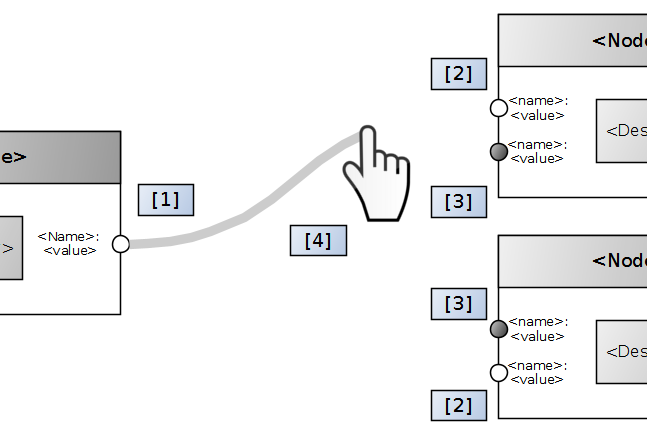
\includegraphics[width=.75\textwidth]{bilder/chapter4/chapter4_3/connectNodes.png}
  \caption{Das Radialmenu mit den fünf verschiedenen Operationsklassen aus Kapitel \ref{subsubsec:eventtrans} zur Auswahl}
  \label{fig:connectNodesInteraction}
\end{figure}
Das Modellieren des Graphen in flowws ist äquivalent mit dem Programmieren von Programmcode. Neben dem Modellieren von \ac{FSM} um das Verhalten von Aktoren zu steuern ist die Hauptarbeit in flowws das Verbinden von Knoten. Das Verbinden von Knoten soll an das Verbinden von Hardware mit Kabeln erinnern (siehe ''Nähe zur Realität''). Aus diesem Grund, wurde sich für eine \textit{Drag-and-Drop}-Interaktion, wie sie in Abbildung \ref{fig:connectNodesInteraction} zu sehen ist entschieden. Hierbei zieht der Endnutzer eine Verbindung von Anfangs-Schnittstelle (a) zu End-Schnittstelle (b). Sobald der Endnutzer diese Interaktion bei (a) beginnt, werden sämtliche potentielle Schnittstellen (b), die mit dem Datentyp von (a) kompatibel sind hervorgehoben. Dadurch soll dem Endnutzer geholfen werden, Fehler zu vermeiden (siehe ''Fehler vorbeugen'').

\subsubsection{Erstellen von Funktionsknoten}

\begin{figure}[h]
  \centering
  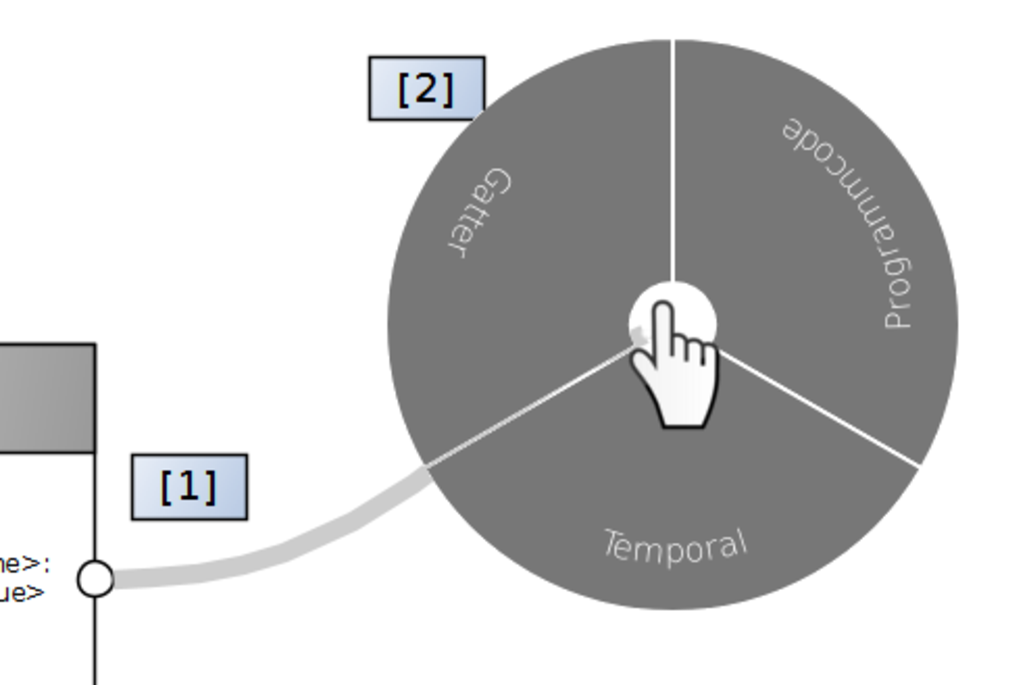
\includegraphics[width=.6\textwidth]{bilder/chapter4/chapter4_3/createNodes.pdf}
  \caption{Das Radialmenu mit den fünf verschiedenen Operationsklassen aus Kapitel \ref{subsubsec:eventtrans} zur Auswahl}
  \label{fig:createNodesInteraction}
\end{figure}
Die Funktionsknoten sind die einzigen Knoten, die in ihrer Existenz nicht an ein physisches Pendant gebunden sind. Aus diesem Grund, werden sie manuell vom Nutzer erstellt und gelöscht. Die Erstellung von Funktionsknoten geschieht mit Hilfe des Radialmenüs. Ein Funktionsblock kann wie in Abbildung \ref{fig:createNodesInteraction} gezeigt auf zwei Weisen erstellt werden: Kontextsensitiv und Kontextunabhängig. \textbf{Kontextunabhängig} können Funktionsknoten auf der ganzen Arbeitsfläche erzeugt werden. Der Benutzer ruft das Radialmenü auf und wählt den gewünschten Knoten aus. \textbf{Kontextsensitiv} ist das Radialmenü Knoten wenn der Endnutzer gerade eine Verbindung erstellt. In diesem Fall, zeigt das Radialmenü nur Optionen an, die für die zu erstellende Verbindung relevant sind. Erstellt der Nutzer bspw. eine Verbindung, die als Quelle den Temperatursensor hat, zeigt das Radialmenü nur Funktionsknoten an, die mit \textit{Number}-Werten (sprich: Temperaturwerten) umgehen können. Für den Endnutzer wird der Erstellungsprozess dadurch übersichtlicher, schneller und weniger fehleranfällig.

\subsubsection{Erstellen von \ac{FSM}}\label{FSMkreieren}


\begin{figure}[h]
  \centering
  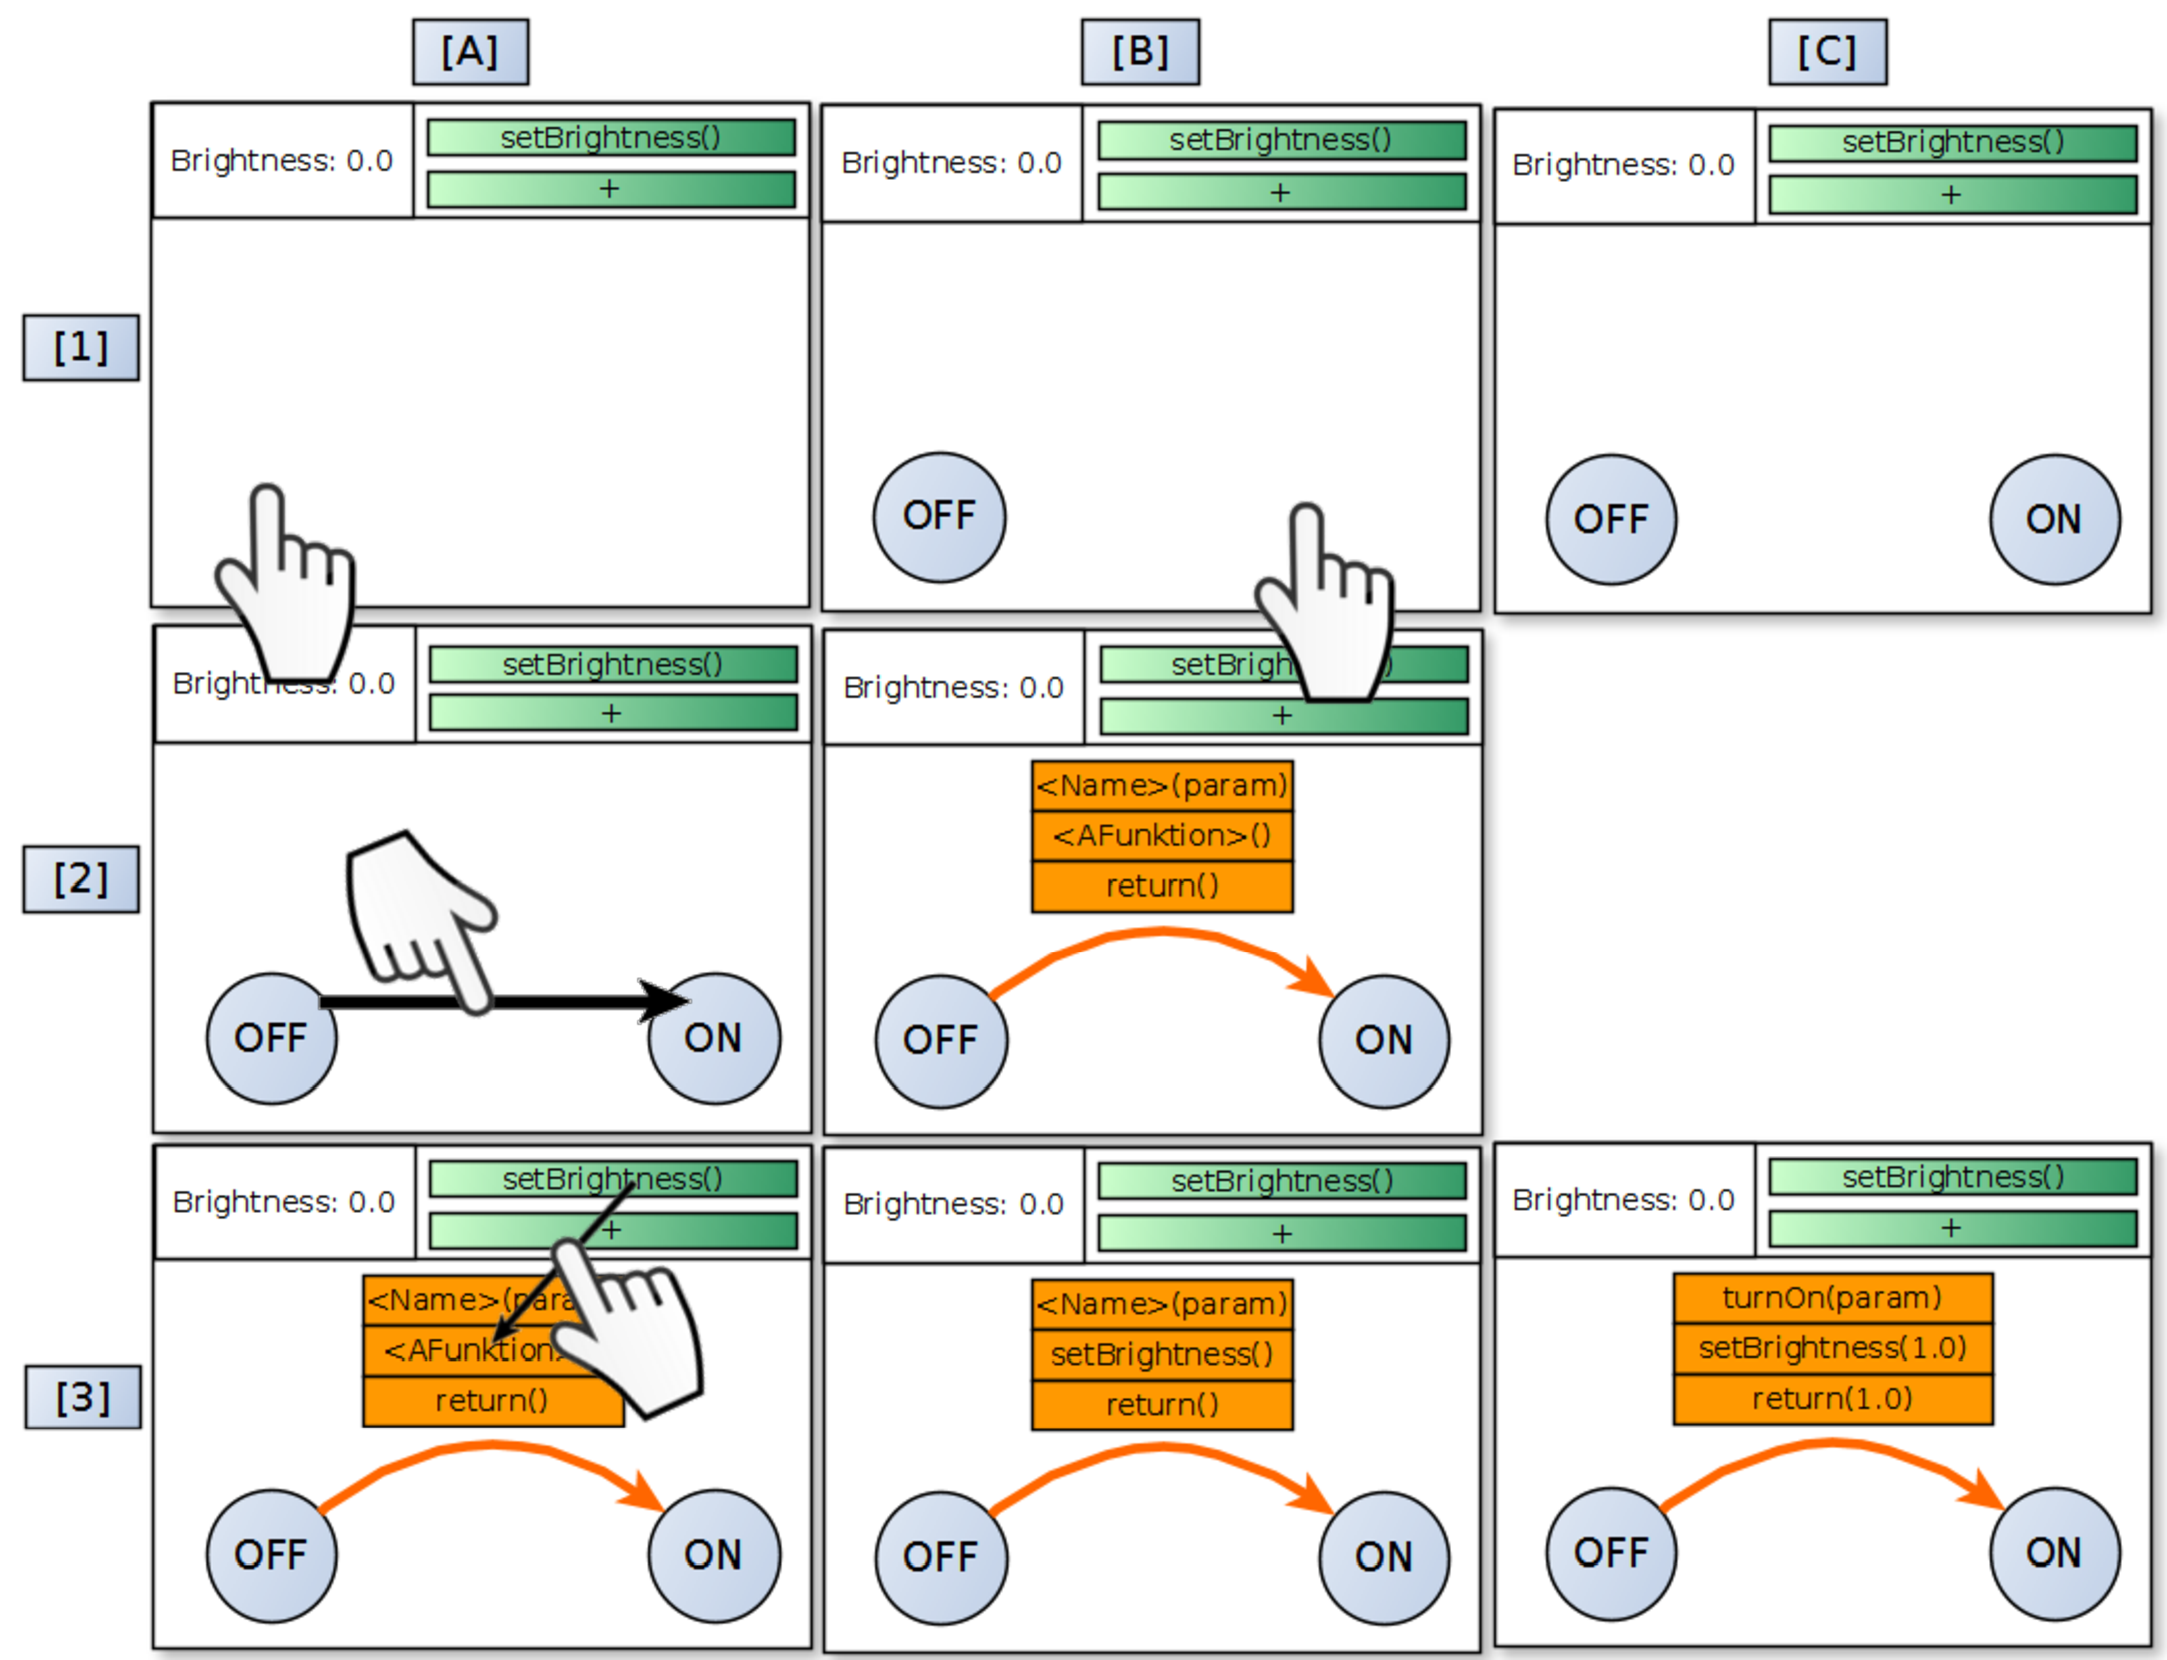
\includegraphics[width=1\textwidth]{bilder/chapter4/chapter4_3/createFsm.pdf}
  \caption{Das Radialmenu mit den fünf verschiedenen Operationsklassen aus Kapitel \ref{subsubsec:eventtrans} zur Auswahl}
  \label{fig:createFSMInteraction}
\end{figure}

Die \ac{FSM} wird in drei Schritten erstellt:
\begin{enumerate}
    \item \textbf{Zustände erstellen und benennen} In [A1] bis [C1] werden durch das Betätigen der Oberfläche Zustände erstellt. Der Endutzer benennt die Zustände und gibt ihnen somit eine symbolischen Bedeutung.
    \item \textbf{Übergänge definieren} Mit einer \textit{Drag-and-Drop}-Interaktion werden vom Endnutzer in [A2] und [B2] die Übergänge zwischen den Zuständen gezogen. Sobald ein valider Übergang entstanden ist bekommt er automatische eine einzigartige Farbe und ein generische Vorlage für die Übergangslogik zugewiesen.
    \item \textbf{Übergangslogik definieren} Die Definition der Übergangslogik geschieht ebenfalls durch \textit{Drag-and-Drop}-Interaktionen. Aktorfunktionen werden hierbei (siehe [A3] bis [C3]) durch den Endnutzer auf die entsprechenden Stellen in der Übergangslogik gezogen. Diese Interaktionen und die manuelle Eingabe der Parameter komplettiert die Programmierung des Aktorknotens.
\end{enumerate}

Es gibt noch weitere Interaktionen die der Endnutzer in flowws durchführen kann, wie das Verwalten von Graphen, das Anordnen der Knoten innerhalb des Graphen oder das Erstellen von Aktorfunktionen. Da diese Interaktionen nicht dazu beitragen Logik für \ac{IoT}-Prototypen zu definieren, werden sie innerhalb dieser Thesis auch nicht behandelt. % Externe Datei einbinden
\chapter{Evaluation und Bewertung}
Im Folgenden wird das Konzept von flowws auf seine Nützlichkeit untersucht und bewertet. Hierfür werden im Vorfeld eine Hypothese aufestellt, welche anhand eines Nutzertests verifiziert bzw. falsifiziert wird.

\section{Hypothese: Mentales Modell}\label{sec:hypothese}
\begin{quote}
    \textit{flowws besitzt ein intuitives Konzeptmodell. State-Machines und Flow-basierte Programmierung unterstützen das mentale Modell der Stakeholder.}
\end{quote}

In dieser These wird aufgestellt, dass flowws Konzeptmodell sich dazu eignet dem Endnutzer ein mentales Modell zu vermitteln, welches ihm erlaubt, cBlocks effektiv zu programmieren. Es ist zu erwarten, dass Probanden, welche die Persona repräsentieren, nach einer minimalen Einweisung, Graphen die in flowws modelliert wurden deuten und das Verhalten von ihnen antizipieren können. Durch das Konzeptmodell von flowws und der graphische Oberfläche wird versucht, an die graphische Denkweise vieler Endnutzer anzuknüpfen zu können und dadurch einen größeren Lerneffekt und mehr Verständnis für die Programmlogik im Vergleich zu textuellen Programmcode zu erzeugen.

%Für das Konzept von flowws wurde sich für eine graphische Oberfläche entschieden. Es wurde dadurch erhofft, an die graphische Denkweise vieler Endnutzer anzuknüpfen zu können und dadurch einen größeren Lerneffekt und mehr Verständnis für die Programmlogik im Vergleich zu textuellen Programmcode zu erzeugen. Die \ac{GUI} erweist sich als effektives Kommunikationsmedium um das Konzeptmodell von flowws mit dem mentalen Modell des Stakeholders zu verbinden.
\section{Aufbau der Evaluation}
Um die Hypothese zu beweisen oder zu widerlegen, werden drei ausgebildete Designer befragt. Für die Befragung, wird den Probanden zwei verschiedene Szenarien gezeigt, welche zwei der drei Szenarien aus Kapitel \ref{sec:szenarien} abbilden.

Den Probanden werden in einem flowws-Prototyp zwei fertige Graphen innerhalb eine flowws-Prototypen gezeigt, die mit den Szenarien \hyperref[szenario1]{S\#1} und  \hyperref[szenario3]{S\#3} (siehe Kapitel \ref{sec:szenarien}) korrespondieren. Die Aufgabe der Endnutzer ist es, die verschiedenen Komponenten des Graphen zu identifizieren, ihre Funktion zu deuten und Rückschlüsse über ihr Verhalten zu ziehen. Wenn die Probanden das Verhalten des Graphen antizipieren können, wird im Dialog elaboriert, ob das mentale Modell, dass der Endnutzer gebildet hat, mit dem Konzeptmodell von flowws übereinstimmt. Wenn der Endnutzer das Verhalten des Graphen nicht antizipieren kann, werden im Dialog die Diskrepanzen zwischen dem Konzept- und dem mentalen Modell erörtert. Der Dialog geschieht anhand eines Fragebogens (siehe Anhang \ref{subsec:fragebogen}), der sich auf die \ac{CD} stützt \cite{blackwell2000cognitive}.

Der \textbf{Aufbau} und \textbf{Ablauf} der Evaluation ist wie folgt:
\begin{enumerate}
    \item Der Proband gibt Angaben zu seinen Merkmalen und schätzt sein Fachwissen hinsichtlich \ac{IoT}-Domäne und Programmierung ab (siehe Anhang \ref{subsec:fragebogen}).
    \item Der Proband liest zusammen mit dem Gutachter den Interview Leitfaden (siehe Kapitel \ref{subsec:leitfaden}) durch. Eventuelle Unklarheiten werden hierbei beseitigt. 
    \item Dem Proband werden nacheinander zwei Graphen gezeigt. Nach jedem Graphen wird anhand eines Fragebogens geprüft, ob der Nutzer die Funktionen der einzelnen Komponenten sowie deren Zusammenspiel deuten kann. Es wird als Erfolg gesehen, wenn der Proband von selbst das abgebildete Szenario beschreiben kann, d.h. er hat verstanden, das eine LED von rot zu gelb zu grün wechselt und somit eine Ampel abbildet. 
    \item Nachdem alle zwei Graphen abgearbeitet worden sind, werden generelle Fragen zum Konzeptmodell gestellt. Hierbei werden Fragen verwendet, die sich an den \textit{Cognitive Dimensions} (siehe Kapitel \ref{tab:cognitivedimensions}) nach \cite{blackwell2000cognitive} orientieren. Ziel ist es dabei grundsätzliche Schwächen, Stärken von flowws, sowie Verbesserungspotential zu identifizieren.
\end{enumerate}

Um die Effektivität des \ac{EUD}-Konzeptes möglichst früh zu prüfen, bevor eine vollständige Implementierung vorliegt, wird die hier beschriebene Evaluation wird auf dem Konzept von flowws in einem frühen Stadium durchgeführt. Die Erstellung eines eigenen Graphen durch den Anwender könnte ergänzend durchgeführt werden, wenn die Implementierung an einer späteren Phase des Projektes abgeschlossen ist. 

\subsection{Prototyp}

\begin{figure}[h]
  \centering
  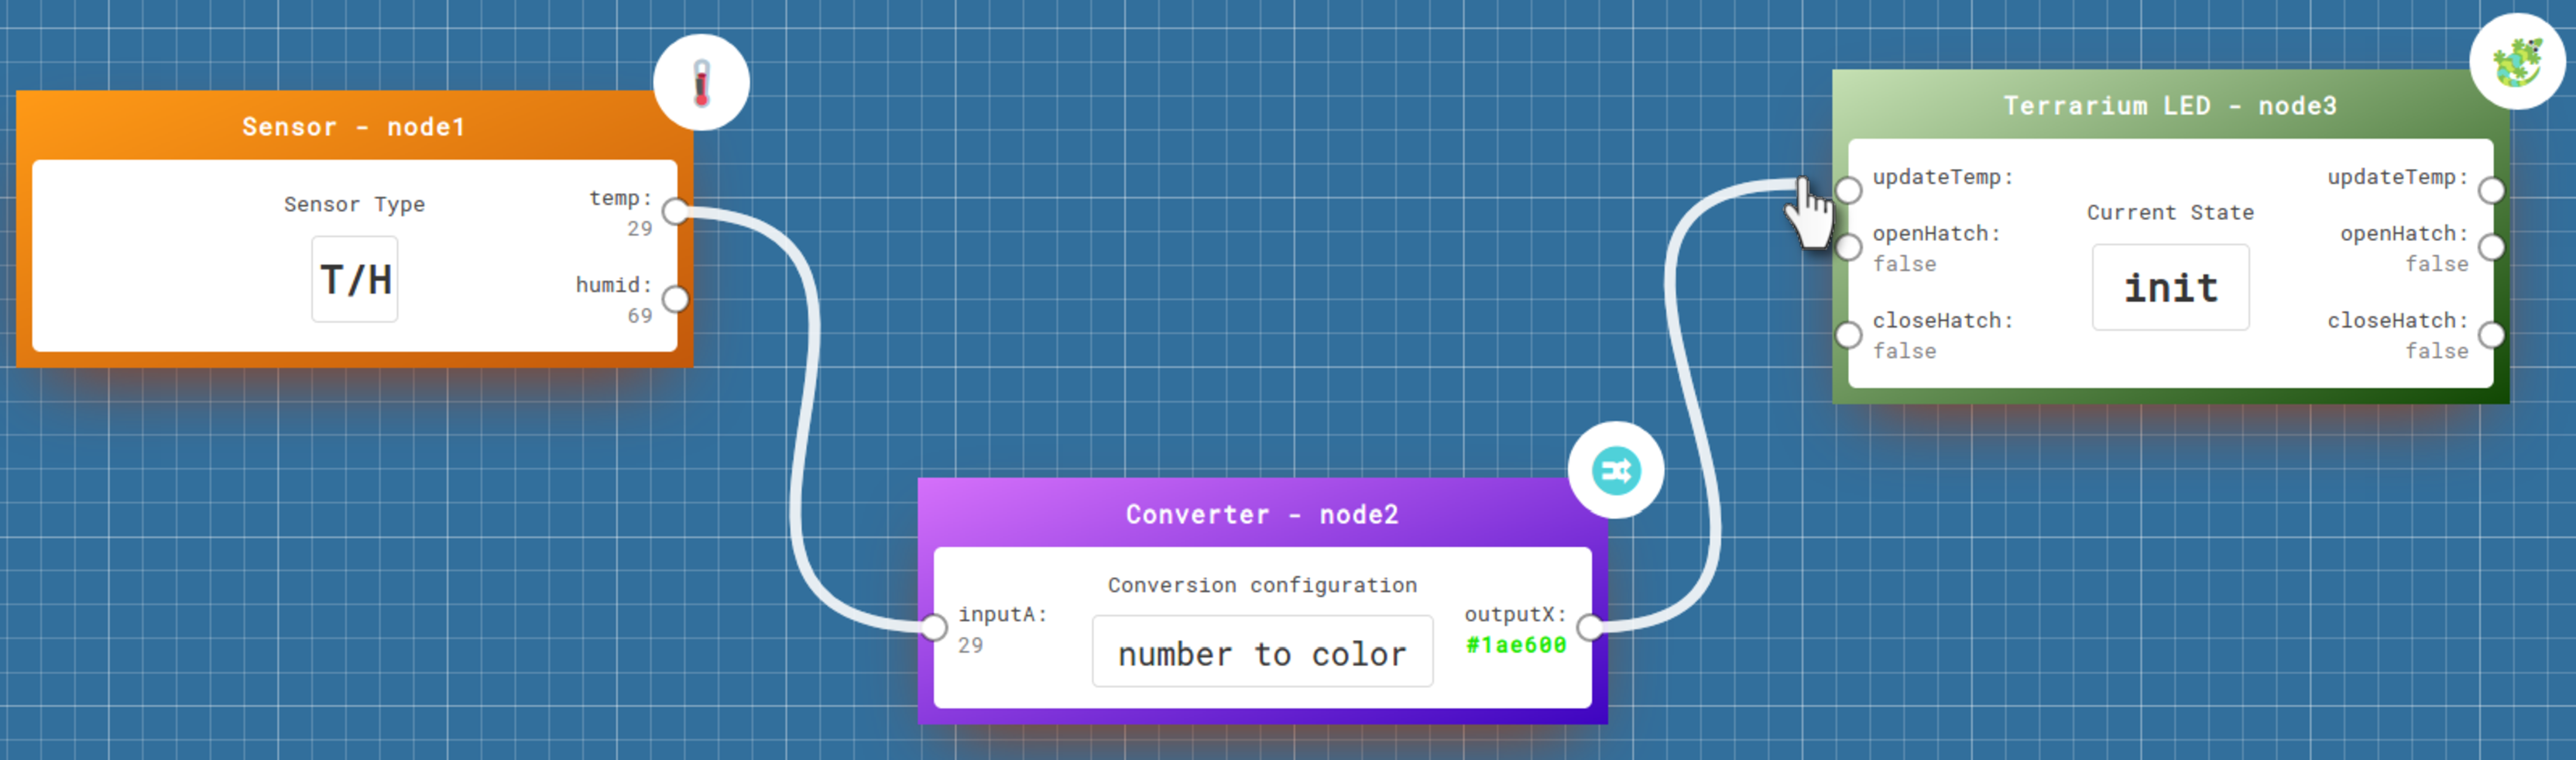
\includegraphics[width=1\textwidth]{bilder/chapter5/screenshotflows.pdf}
  \caption{Screenshot des flowws-Prototyps}
  \label{fig:genericnode}
\end{figure}

Für die Evaluation wurde im Zuge dieser Thesis eine prototypische Implementierung von flowws erstellt. Der Prototyp kann die grundlegenden Elemente (Sensor-, Aktor- und Funktionsknoten, Verbindungen) von flowws darstellen und animieren. Darüber hinaus, lassen sich die Elemente miteinander kombinieren und die Signalverarbeitung des Graphen simulieren.

Der Sourcecode wurde als \textit{Webapp} mit dem React-Framework\footnote{\url{https://reactjs.org/} - besucht September 2018} erstellt und steht in einem \textit{Github-Repository}\footnote{\url{https://github.com/chrbrt/flowws} - besucht September 2018} zur freien Verfügung und Erweiterung.
\section{Durchführung der qualitativen Evaluation}

Die Durchführung des Benutzertests geschah mit drei Personen, von denen zwei Personen, Designer (Master of Arts und Diplom). Die andere Person arbeitet im Bereich der \textit{Business-Communication}/Marketing (\textit{Master of Arts}), besitzt allerdings praktische Erfahrung im Bereich \textit{Product-Design} durch aktiver Beteiligung an mehreren Design-Projekten. Sie sind alle weiblich, zwischen 22-35 Jahren alt, und besitzen umfangreiches Wissen über Designmehthoden (bspw. \textit{Rapid-Prototyping}, \textit{Design-Thinking}, etc.). Die Erfahrung der Benutzergruppe im Bereich \ac{IoT} und \textit{Soft\-ware-Engineering} ist gering und reicht von ''\textit{unbedarft}'' bis ''\textit{Grundkenntnisse} mit Arduino''. Die Benutzergruppe reflektiert somit den Charakter der Persona ''Laura'' (siehe Kapitel \ref{sec:persona}) gut.

\subsection*{Verständnis Datenfluss-Komponente des flowws-Graphen}
Die Datenfluss-Kom\-po\-nen\-te ist das initiale Element, dass der Benutzer bei flowws erblickt. Es wurde die \textit{funktionale Aussagekraft}, \textit{Sichtbarkeit}, die \textit{fortwährende Evaluation} des Programmes und die Qualität der \textit{Abstraktionen} (siehe \ref{tab:cognitivedimensions}) der einzelnen Knoten evaluiert. Folgende Beobachtungen wurden gemacht: 
\begin{itemize}
    \item Zwei von drei Probanden konnten die virtuellen Knoten mit denen der physischen Knoten abgleichen.
    \item Alle Probanden identifizieren, das Signale zwischen den einzelnen Knoten gesendet werden.
    \item Eine der Probanden gab an, sie dachten, dass Funktionsknoten auch physische Knoten repräsentieren (z.B. \textit{Timer}-Knoten).
    \item Alle Probanden konnten durch das Vergleichen von In- und Output, auf die Funktionen der Knoten schließen.
    \item Zwei der drei Probanden konnte die Arbeitsweise des ersten Datenflussgraphen deuten, ohne vom Gutachter darauf hingewiesen zu werden. Der Graphen des zweiten Szenarios konnte nur teilweise gedeutet werden. Erst nach Erläuterung des Zieles des Prototypen, konnten der Sinn, der einzelnen Elemente gedeutet werden. 
    \item Die Person mit der meisten Erfahrung in Software-Engineering wurde durch ihr eigenes Wissen von Kontrollstrukturen abgelenkt. Sie deutete die Verbindungen zwischen den Knoten als bedingte Verzweigungen. Die zwei anderen Probanden besaßen aufgrund ihrer naiveren Betrachtungsweise, weniger Probleme, die Funktion des Graphen zu identifizieren.
    \item Ein Proband bemängelte, dass generische Knoten nicht benannt sind (bspw. anstatt ''Taster'', ''Taster für Terrariumöffnung'').
\end{itemize}

\subsection*{Verständnis für Aktoren/\ac{FSM}} 
Die Steuerung der Aktor-\ac{FSM} ist die zweite Säule des flowws-Konzepts. Ähnlich wie bei der Datenfluss-Komponente, wurden die Komponenten des Aktors auf Basis der gleichen \ac{CD} evaluiert. Die Probanden bemerkten Folgendes:
\begin{itemize}
    \item Alle Probanden konnten den Aktor als solchen identifizieren.
    \item Ohne Einweisung, konnten die Probanden nur wenig mit der Darstellung der \ac{FSM} anfangen. Nach kurzer Erläuterung, wurde das Prinzip von allen Probanden angenommen.
    \item Die Benutzer hatten Probleme mit der rein symbolischen Benennung von Zuständen. -- ''\textit{Warum ist 'Klappe geöffnet' ein Zustand innerhalb des LED Aktors?}'' 
    \item Ein Proband hat erwartet, dass die zeitliche Steuerung innerhalb des Aktors selbst stattfindet, anstatt in einem separaten Funktionsknoten.
    \item Ein Proband konnte den Rückgabewert (\texttt{return(<wert>)}) dem Ausgang des Aktors zuordnen, alle anderen Probanden hatten Probleme mit dem Konzept eines Rückgabewerts.
    \item Nach einer Erläuterung konnten zwei von drei Probanden das Verhalten des Aktors auf willkürliche Eingangssignale vorhersagen. Dabei beschrieben sie implizit die Fähigkeit von \acp{FSM}, Signale zu priorisieren.
\end{itemize}

\subsection*{Verständnis für Darstellung von flowws}
\begin{itemize}
    \item Farbliche Aufteilung der Knoten in Sensor, Funktion und Aktor wurde von allen Benutzern sofort unterbewusst angenommen.
    \item Die Farben der Aktor-Eingänge sollten mit den Farben der Übergängen übereinstimmen.
    \item Animationen beim Ändern von In- und Output-werten sehr hilfreich. Auch die Animation der Verbindungen half den Probanden bei dem Nachverfolgen der Daten.
    \item Animationen sind zum Teil zu schnell. -- ''\textit{Ich habe gesehen, dass sich etwas verändert hat, aber nicht genau was.}''
    \item Eine Funktion zum pausieren der Sensoren wäre hilfreich.
    \item Die Darstellung und Animationen von flowws erinnern laut Probanden an Rohrleitungen und an Dia\-lyse\-ge\-räte.    
    \item Der Verlust eines Indexes, mit sämtlichen Funktionsknoten machte einen einen Probanden unsicher, da keine Knoten zum Vergleichen bereitstanden. Ein Index würde einen besseren Gesamtkontext für die Funktionsknoten bieten. 
\end{itemize}
\subsection*{Sonstige Bemerkungen} 
\begin{itemize}
    \item Zwei von drei Probanden fingen an, mit der Konfigurationen der Funktionsknoten zu explorieren, ohne dass sie dazu aufgefordert wurden und der Prototyp dieses nur im geringen Maße unterstützt.
    \item Die Probanden besitzen Schwierigkeiten mit nicht-deskriptiven Daten. Ein Proband konnte nichts mit einem Helligkeitswerte von 1.0 des LED-Aktors anfangen, da sie die prozentuale Skala der Eigenschaft nicht intuitiv herleiten konnte.
    \item Einem der Probanden war es möglich die Fehlkonfiguration eines Funktionsknotens, durch den Gutachter, auszumachen.
\end{itemize}

\section{Wertung der Ergebnisse}

\subsection{Erfüllung der Anforderungen}
Die Evaluation hat neben dem Beweis der Hypothese, auch Aufschluss über die Erfüllung der Anforderungen aus Kapitel \ref{sec:anforderungen} gegeben. Im Folgenden wird im Anbetracht der Ergebnisse der Nutzertests diskutiert, in wie weit flowws den Anforderungen gerecht wird und welche Anforderungen noch weitere Evaluation benötigen.

\subsubsection{Erfüllen von funktionale Anforderungen}
Die funktionalen Anforderungen aus Kapitel \ref{subsec:fanf} bezogen sich hauptsächlich auf die Verarbeitung von Daten. Vergleichs-, bool'sche und zeitgesteuerte Operationen (siehe \hyperref[tab:fanf]{FA\#1-3}) sowie die Konvertierung von Signalen (\hyperref[tab:fanf]{FA\#7}) werden von Funktionsknoten abgebildet. Das Auslesen und Anzeigen von Sensordaten (\hyperref[tab:fanf]{FA\#4}) geschieht automatisch über die Sensorknoten. Das Konzept zum Ansteuern von Aktoren und das Programmieren von Aktoren (\hyperref[tab:fanf]{ FA\#5} u. \hyperref[tab:fanf]{ FA\#6}) wurden in Kapitel \ref{subsubsec:evebtkonsumierung} und Kapitel \ref{FSMkreieren} ausführlich beschrieben.

\subsubsection{Erfüllen nicht funktionalen Anforderungen}
\paragraph{NFA \#0: Parallel und Sequentielles....} Durch das Konzeptmodell von flowws, welches Datenfluss- und \ac{FSM}-Programmierung kombiniert konnte diese Anforderung erfüllt werden. Die Nutzertests haben angedeutet, dass potentielle Endnutzer paralleles und sequentielles Verhalten, ohne hohen kognitiven Aufwand innerhalb von flowws, begreifen können.

\paragraph{NFA \#1: Daten und State ...} flowws visualisiert Daten und Zustand des Programms an mehreren Stellen. Jeder Knoten zeigt seine aktuellen Ein- und Ausgangs Daten an, der Fluss von Daten wird animiert und der Zustand von Aktoren wird dargestellt (siehe Kapitel\ref{sec:graphischesmodell}). Dadurch entsteht ein Gefühl von dynamik, die es dem Endnutzer erlaubt zu Laufzeit das Verhalten des Programms nachzuvollziehen. Dies wurde von den Nutzertests bestätigt.

\paragraph{NFA \#2: Schneller erlernbar...} Durch die visuelle Darstellung von flowws wird sich erhofft, dass das visuelle Denken von Menschen unterstützt wird und somit sich der Lernaufwand reduziert. Die Nutzertests haben Aufschluss über die Verständlichkeit von flowws geliefert. Um einen besseren Aufschluss über die Erlernbarkeit von flowws zu erreichen, müssen weitere Prototypen gebaut werden, welche es Probanden erlauben eigene Graphen zu modellieren.

\paragraph{NFA \#3: Schnelle modifzierung...} Die Komponenten von flowws (Sensoren, Funktionen, Aktoren) sind allesamt in einzelne Knoten gekapselt und durch klar definierte Schnittstellen miteinander verbunden. Funktions- und Aktorknoten lassen sich noch individuell konfigurieren. Dies lädt den Endnutzer dazu ein, Knoten auszutauschen und zügig mehrere Alternativen zu einem bestehenden flowws-Graphen zu erproben. Dieses Verhalten konnte auch schon in den Nutzertests nachgewiesen werden.

\paragraph{NFA \#4: Fehlerprävention} Der größte Teil der Programmierung in flowws stellt das Verbinden von Knoten. flowws versucht durch kontextuelles Markieren von kompatiblen Schnittstellen und dem kontextuellen Auswählen von kompatiblen Funktionsknoten, die Fehlerzahl im Voraus zu reduzieren. 

\paragraph{NFA \#5: Erweiterbarkeit von Komponenten} flowws kann auf zwei Ebenen von Experten erweitert werden: zum einen durch benutzerdefinierter Logik von Funktionsknoten und zum anderen durch definieren von Aktorfunktionen. Diese beiden Gegebenheiten sollten es fortgeschrittenen Endnutzern erlauben, eine größere Bandbreite von Szenarien abzudecken. Des Weiteren ist flowws \textit{Open Source} und somit von Software-Ingenieuren erweiterbar und anpassbar.


\section{Erfüllung der Anforderungen und Ziele}
- Erfüllung von funktionalen Anforderungen
- Erfüllung von nicht funktionalen Anforderungen
- Erfüllung von Zielen



 % Externe Datei einbinden
\chapter{Reflexion \& Zukünftige Arbeiten}
Im letzten Kapitel wird noch einmal über die Inhalte und Ergebnisse dieser Arbeit reflektiert. Zuletzt wird das Erreichen der Forschungsfragen und die daraus resultierenden Folgefragen diskutiert.

Diese Arbeit hatte zum Ziel, das Konzept für ein \ac{EUD}-Werkzeug zu erstellen, dass die spezifischen Anforderungen von \ac{IoT} und den Projekt-Kontext der \acp{cBlock} aufgreift. Die Arbeitet hat sich aus diesem Grund in vier Teile aufgegliedert:

\begin{itemize}
    \item \textbf{Wissenserhebung} In Kapitel \ref{GrundlagenSOTA} wurden die fachlichen Grundlagen in \ac{IoT} und \ac{EUD} gelegt. Hierbei wurden die unterschiedlichen Aspekte, Komponenten und Charakteristiken von \ac{IoT} definiert. Ziel hierbei war es, ein Gefühl für \textit{Smart Devices} und ihre Art der Kommunikation zu erlangen, um später eine adäquate Metapher für flowws, definieren zu können. Ebenfalls wurde der Begriff der \ac{EUD} geklärt. Das Ergebnis des Kapitels, korrespondiert direkt mit der ersten Forschungsfrage und kulminiert mit einer Analyse von drei populären \ac{EUD}-Paradigmen und ihre Implementierungen in der \ac{IoT}-Domäne.
    \item \textbf{Analyse} Kapitel \ref{chapter:analyse} bestand aus einer zweigeteilten Analyse, die die generellen Probleme von \acp{EUD} im \ac{IoT} abstrahiert und dem Endnutzer selbst mit seinen Problemen charakterisiert. Das Ergebnis zielt auf die Beantwortung der Forschungsfrage \#1 (siehe Kapitel \ref{sec:1_zielsetzung}) ab und ist eine Spezifikation von Vision, Zielen und Anforderungen eines \ac{EUD}-Werkzeugs, welches sich Gesamtkontext dieser Thesis orientiert.
    \item \textbf{Konzeption} Das Ziel von Kapitel \ref{chapter:konzeption} war es, sämtliche Probleme und Anforderungen in ein Konzeptmodell umzusetzen. Das Ergebnis wurde ''flowws'' getauft. Es ist eine graphische Programmiersprache Datenfluss-Logik und \ac{FSM}-Logik zu kombiniert um somit die spezifischen Rahmenbedingungen des Kontext erfüllt und somit Forschungsfrage \#2 (siehe Kapitel \ref{sec:1_zielsetzung}) beantwortet.
    \item \textbf{Evaluation} Die Evaluation des Konzeptmodells wurde anhand eines Nutzertests mit einem \ac{EUD}-Prototyp und geeigneten Endnutzern, durchgeführt. Ziel hierbei war es festzustellen, ob das Konzeptmodell von flowws mit dem mentalen Modell der Endnutzer vereinbar ist. Das Ergebnis ist die Antwort auf Forschungsfrage \#3 (siehe Kapitel \ref{sec:1_zielsetzung}) , indem bewiesen wurde, dass flowws eine vielversprechendes Konzeptmodell besitzt, welches die fachlichen und technischen Anforderungen unterstützt und gleichzeitig für den Endnutzer in kurzer Zeit nachvollziehbar ist.
\end{itemize}

Das Endprodukt dieser Thesis ist das \ac{EUD}-Konzept, das hinter flowws steht. Das Konzept hat gezeigt, dass eine Kombination von Datenfluss- und \ac{FSM}-Pro\-gram\-ma\-tik nicht nur eine treffende Abstraktion bzw. Metapher für \ac{IoT} ist, sondern auch ein guter Kompromiss zwischen Funktionsumfang und Erlernbarkeit bietet. Es wurde ein Prototyp entwickelt, welches die Nachvollziehbarkeit des Konzepts bewiesen hat. Dies ist ein guter Ansatzpunkt für weitere Arbeiten in diesem Kontext:

\begin{itemize}
    \item \textbf{Funktionelle Konzeption:} Eine komplettes \ac{EUD}-Werkzeug ähnelt einer \ac{IDE}. Sie besitzt Funktionalitäten, die der Endnutzer ausnutzen kann, um Programme zu erstellen, zu testen und zu verwalten. Es stellt sich also zur Frage, welche weiteren Funktionen benötigt werden, um aus flowws ein produktives Werkzeug zu machen.
    
    \item \textbf{Technische Konzeption:} Die momentane Implementierung von flowws beschränkt sich auf einen \textit{Experience-Prototyp}. Dieser ist eine reine Darstellung des Konzepts und dient um die \ac{UX} von flowws zu evaluieren. Die technische Umsetzung von flowws wurde in dieser Thesis nicht behandelt, ist aber aufgrund der Interaktionen verschiedener Teilsysteme ein nicht-triviale Problemstellung. Folglich kann eine technische Anforderungsanalyse, Architekturbeschreibung und Implementierung, die cBlocks integriert, ein Ziel zukünftiger Arbeiten sein. 
    
    \item \textbf{Erweiterte Evaluation} Eine der möglichen Kritiken der Evaluation ist die Größe der Stichprobe. Drei Partizipanten sind nicht ausreichend, um eine nachhaltige Aussage zu treffen. Nachfolgende Arbeiten könnten die Anzahl der Probanden erhöhen um eine allgemeingültige Aussage über das Konzeptmodell von flowws zu treffen. Des Weiteren, war die hier aufgeführte Evaluation rein passiv, sprich der Nutzer hat nicht aktiv mit flowws interagiert. Zukünftige Arbeiten könnten ausführlichere Studien beinhalten, die den Erstellungsprozess von Graphen in flowws auf seine Nutzerfreundlichkeit überprüfen.
\end{itemize} % Externe Datei einbinden
% ------------------------------------------------------------------

\label{lastpage}

% Neue Seite
\cleardoublepage

% Backmatter mit normalem Zeilenabstand setzen
\singlespacing

% Römische Ziffern für die "Back-Matter", fortlaufend mit "Front-Matter"
\pagenumbering{roman}
\setcounter{page}{\value{frontmatterpage}}

% Abkürzungsverzeichnis
\addchap{\hsmaabbreviations}
\begin{acronym}
\acro{IoT}{Internet of Things}
\acro{cBlock}{connected Block}
\acro{EUD}{End-User Development}
\acro{EUP}{End-user Programming}
\acro{EUC}{End-user Computing}
\acro{EUSE}{End-user Software Engineering}
\acro{Ubicomp}{Ubiquitous computing}
\acro{UX}{User Experience}
\acro{UI}{User Interface}
\acro{DSL}{Domain Specific Language}
\acro{HDL}{Hardware Definition Language}
\acro{ITU}{International Telecommunication Union}
\acro{6LoWPAN}{IPv6 over Low power Wireless Personal Area Network}
\acro{WSAN}{Wireless Sensor and Actor Network}
\acro{GUI}{Graphical User Interface}
\acro{SOA}{Service Oriented Architecture}
\acro{CD}{Cognitive Dimensions}
\acro{PBD}{Programming-by-Demonstration}
\acro{TAP}{Trigger-Action-Programmierung}
\acro{USP}{Unique Selling Point}
\acro{CEP}{Complex Event Processing}
\acro{VPS}{visuelle Programmiersprache}
\acro{DBP}{Datenfluss-basierter Programmierung}
\acro{KBP}{Kontrollfluss-basierter Programmierung}
\acro{FSM}{Finite-State-Machine}
\acro{IDE}{Integrated Development Environment}


\acroplural{VLP}[VLPs]{visuelle Programmiersprachen}
\end{acronym}

% Tabellenverzeichnis erzeugen
\cleardoublepage
\phantomsection
\addcontentsline{toc}{chapter}{\hsmalistoftables}
\listoftables

% Abbildungsverzeichnis erzeugen
\cleardoublepage
\phantomsection
\addcontentsline{toc}{chapter}{\hsmalistoffigures}
\listoffigures

% Listingverzeichnis erzeugen
\cleardoublepage
\phantomsection
\addcontentsline{toc}{chapter}{\hsmalistings}
\lstlistoflistings

% Literaturverzeichnis erzeugen
\begin{flushleft}
\printbibliography
\end{flushleft}

% Index ausgeben. Wenn Sie keinen Index haben, entfernen Sie einfach
% diesen Teil.
\cleardoublepage
\phantomsection
\addcontentsline{toc}{chapter}{\hsmaindex}
\printindex

% Anhang. Wenn Sie keinen Anhang haben, entfernen Sie einfach
% diesen Teil.
\appendix
\chapter{Anhang}

\section{Umfrage}
\subsection{Interview-Leitfaden}\label{subsec:leitfaden}
Vielen Dank, dass sie sich Zeit genommen haben, in dieser Evaluation zur Benutzerfreundlichkeit von flowws teilzunehmen.

flowws ist eine Softwareumgebung, die es sich zum Ziel gesetzt hat, die Programmierung von Smart Devices und Connected Products (bspw. NEST-Thermostat, Fitbit, Hue Glühbirnen, etc.) zu erleichtern und auch Nicht-Technikern zu ermöglichen. Um dieses Ziel zu erreichen, wird flowws in Verbindung mit cBlocks verwendet, um Prototypen im \ac{IoT} Bereich zu erstellen. Zwar besitzen diese Prototypen nicht das Aussehen des finalen Produkts, sollen aber das gleiche Verhalten abbilden. 

cBlocks sind physikalische Bausteine, welche die einzelnen Elektronikbausteine repräsentieren, aus denen sich Smart Devices zusammensetzen: Sensoren und Aktoren. cBlocks spalten sich in zwei Gruppen auf:
\begin{itemize}
    \item \textbf{Sensor-cBlocks} transformieren physische Signale (Licht, Schall, Temperatur, etc.) in elektronische Signale um.
    \item \textbf{Aktor-cBlocks} sind bspw. Lautsprecher und LEDs. Sie wandeln elektronische Signale in physikalische Signale (LED aufleuchten, mit Lautsprecher Geräusch abspielen, etc.) um.
\end{itemize}
Ein Beispiel für einen Prototyp könnte ein intelligenter Rauchmelder sein. Ein solcher Rauchmelder würde aus drei cBlocks gebaut werden, welche CO2-Sensor, Temperatur-Sensor und Lautsprecher-Aktor besitzen. Die Logik nach der sich der Rauchmelder verhält muss ihm einprogrammiert werden. Hierbei kommt flowws ins Spiel.

flowws verbindet Sensor- und Aktor-cBlocks, indem es die Daten, welche die Sensoren erzeugen umwandelt, und damit das Verhalten der Aktoren steuert. Für die Umwandlung von Daten kommt eine dritter, rein virtueller, Block zum Einsatz: der Wandler/Transducer. Ein Wandler würde im oberen Beispiel die Temperatur-Daten und CO2-Konzentration der Sensor-cBlocks kombinieren und darüber entscheiden ob der Lautsprecher-cBlock Alarm schlagen soll.

Der Nutzer verwendet flowws, um genau diese Art von Logik auf einer graphischen Oberfläche zu programmieren.

Uns interessiert die Verständlichkeit von flowws. Aus diesem Grund, werden dir im Folgenden mehrere Programme in flowws gezeigt. Wobei es deine Aufgabe ist, die Funktionen der einzelnen Elemente, ihre Aufgaben zu deuten und ihr Verhalten vorherzusagen.

\subsection{Fragebogen}\label{subsec:fragebogen}
\begin{table}[H]
\caption{Angaben zur Person}
\label{tab:questPers}
\begin{tabularx}{\textwidth}{lX}
\hline
\rowcolor[HTML]{EFEFEF} 
Charakteristik                              & Ausprägung                                \\ \hline
Name                                        &                                           \\ \hline
Geschlecht                                  &                                           \\ \hline
Alter                                       &                                           \\ \hline
Beruf/Studium                               &                                           \\ \hline
\end{tabularx}
\end{table}


\begin{table}[H]
\caption{Angaben zur Erfahrungen}
\label{tab:questErf}
\begin{tabularx}{\textwidth}{Xccc}
\hline
\rowcolor[HTML]{EFEFEF} 
Erfahrung mit...                              & & Ausprägung                             &   \\ \hline
...IoT & unbedarft & \Circle \: \Circle \: \Circle \: \Circle \: \Circle \: \Circle & selbst schon entwickelt  \\ \hline
...Designmethoden & unbedarft & \Circle \: \Circle \: \Circle \: \Circle \: \Circle \: \Circle & Designexperte  \\ \hline
...Software-Engineering & unbedarft & \Circle \: \Circle \: \Circle \: \Circle \: \Circle \: \Circle & Informatik Studium \\ \hline
...Zustandsautomaten & unbedarft & \Circle \: \Circle \: \Circle \: \Circle \: \Circle \: \Circle & schon Programmiert \\ \hline
...Datenfluss-Programmierung & unbedarft & \Circle \: \Circle \: \Circle \: \Circle \: \Circle \: \Circle & schon Programmiert \\ \hline
\end{tabularx}
\end{table}

\newpage

\subsubsection{Fragen zu Szenarios}
Welche Komponenten sehen sie im Programm?\\
\noindent\rule{\textwidth}{1pt}
\noindent\rule{\textwidth}{1pt}
\noindent\rule{\textwidth}{1pt}

Welche Aufgaben haben diese Komponenten? Wie reagieren sie auf eingehende Signale?\\
\noindent\rule{\textwidth}{1pt}
\noindent\rule{\textwidth}{1pt}
\noindent\rule{\textwidth}{1pt}

Was ist der Aktor wie verhält er sich auf eingehende Signale? Welche sendet er aus?\\
\noindent\rule{\textwidth}{1pt}
\noindent\rule{\textwidth}{1pt}
\noindent\rule{\textwidth}{1pt}

Wann hat das Programm entgegen ihren Vermutungen gehandelt?\\
\noindent\rule{\textwidth}{1pt}
\noindent\rule{\textwidth}{1pt}
\noindent\rule{\textwidth}{1pt}

\newpage
\subsubsection{Generelle Fragen}
\textbf{Diffuseness}: Sagen Programme in flowws direkt, was sie machen?\\
\noindent\rule{\textwidth}{1pt}
\noindent\rule{\textwidth}{1pt}
\noindent\rule{\textwidth}{1pt}

\textbf{Closeness o. M.}: Inwieweit unterscheidet sich die Notation des flowws-\\Programms, von ihren Erwartungen?\\
\noindent\rule{\textwidth}{1pt}
\noindent\rule{\textwidth}{1pt}
\noindent\rule{\textwidth}{1pt}

\textbf{Role-Express.}: Konnten sie die Aufgaben der einzelnen Komponenten im Gesamtkontext deuten?\\
\noindent\rule{\textwidth}{1pt}
\noindent\rule{\textwidth}{1pt}
\noindent\rule{\textwidth}{1pt}

\textbf{Prog Eval}: Hat es flowws ihnen ermöglicht zu jeder Zeit nachzuvollziehen, wie das Ergebnis des Programmes ist.\\
\noindent\rule{\textwidth}{1pt}
\noindent\rule{\textwidth}{1pt}
\noindent\rule{\textwidth}{1pt}

\textbf{Impro}: Denken sie es gibt konkrete Möglichkeiten flowws zu verbessern? Wenn ja, wie?\\
\noindent\rule{\textwidth}{1pt}
\noindent\rule{\textwidth}{1pt}
\noindent\rule{\textwidth}{1pt}
\newpage

\subsection{Szenario \#1}\label{anhang:szenario1}
\begin{figure}[H]
    \centering
    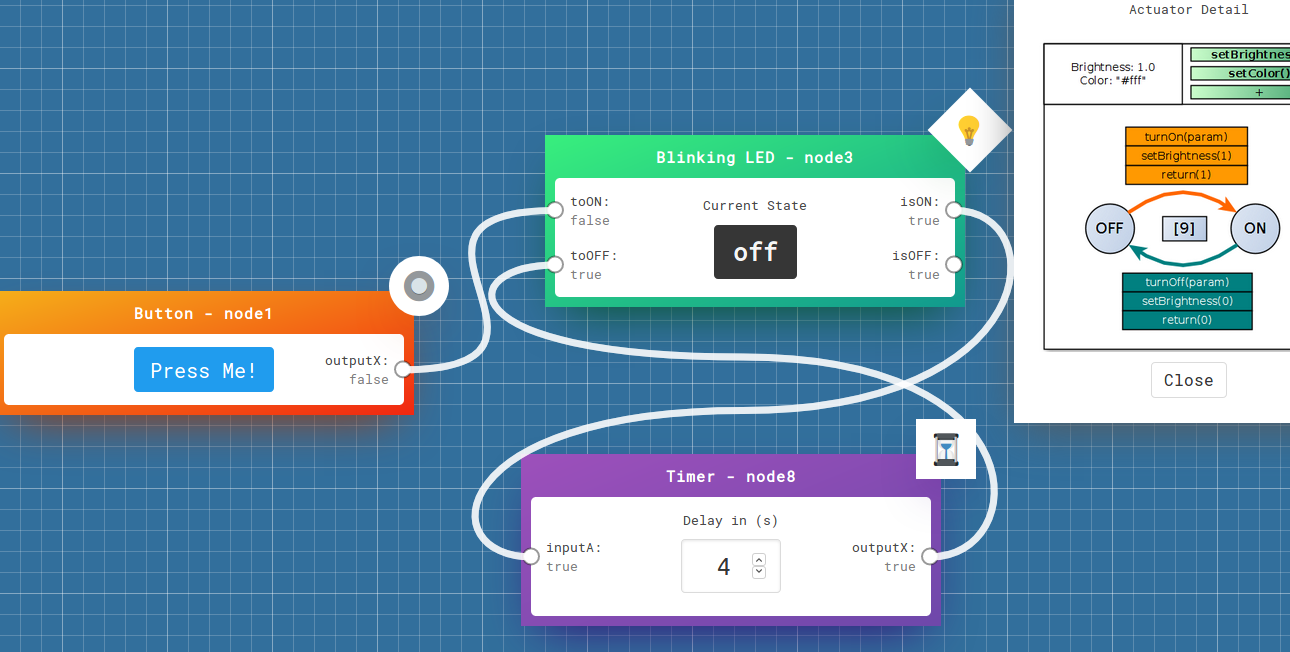
\includegraphics[width=1\textwidth]{bilder/Anhang/timerclock_cut.png}
    \caption{Szenario \#1: Bestehend aus Taster-Sensorknoten, LED-Aktorknoten und Timer-Funktionsknoten.}
    \label{fig:szenario1}
\end{figure}
Dieser Graph (siehe \ref{fig:szenario1}) bildet die Zeitschaltuhr aus Szenario \#1 (siehe Kapitel \ref{szenario1}) ab. Das Szenario besteht aus drei Elementen und verwendet dabei jeden Typ von Knoten. 
Ziel dabei ist es, das der Endnutzer die einzelnen Elemente identifiziert und ihr Zusammenspiel erklärt. Es ist insbesondere interessant, ob der Proband realisiert, dass der Aktor seinen Zustand dem Rest des Graphen mitteilt und somit das Verzögerte ausschalten der LED ermöglicht.

\subsection{Szenario \#2}\label{anhang:szenario2}
\begin{figure}[H]
    \centering
    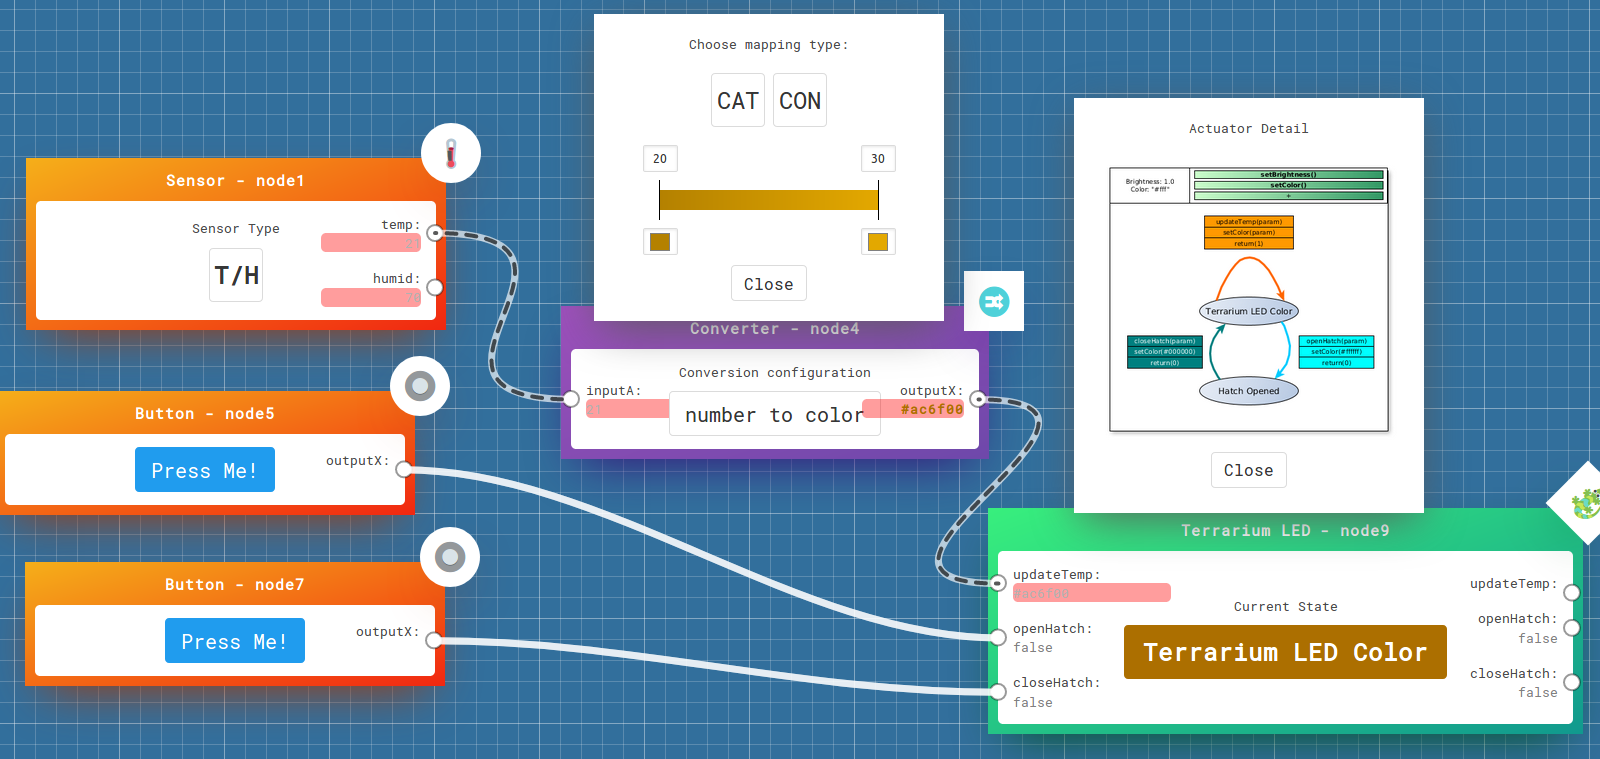
\includegraphics[width=1\textwidth]{bilder/Anhang/terrariumszenario_cut.png}
    \caption{Szenario \#2: Bestehend aus zwei Taster-Sensorknoten, LED-Aktorknoten und Konverter-Funktionsknoten}
    \label{fig:szenario3}
\end{figure}
In Abbildung \ref{fig:szenario3} wird das Terrarium Szenario \#3 von Kapitel \ref{szenario3} im flowws-Prototyp abgebildet. Das Terrarium regelt die Helligkeit abhängig von der Temperatur innerhalb des Terrariums automatisch.
Wird das Terrarium geöffnet, wird ein Taster betätigt und erhellt sich das Terrarium auf die maximale Stufe. Sobald das Terrarium wieder geschlossen wird, wird ein zweiter Taster betätigt und das Terrarium regelt sich wieder anhand des Temperatur-Sensors. 

Der Proband muss hierbei, wie im vorherigen Beispiel, die einzelnen Knoten identifizieren. Gleichzeitig soll der Proband die komplexere Aktorlogik verstehen. Dazu gehört, dass der LED-Aktor eine Signalpriorisierung vornimmt, sobald das Terrarium geöffnet ist.
\newpage
\newpage
\section{Funktionsknoten}\label{anhang:funktionsknoten}
\begin{figure}[h]
\centering
\begin{subfigure}{.5\textwidth}
  \centering
  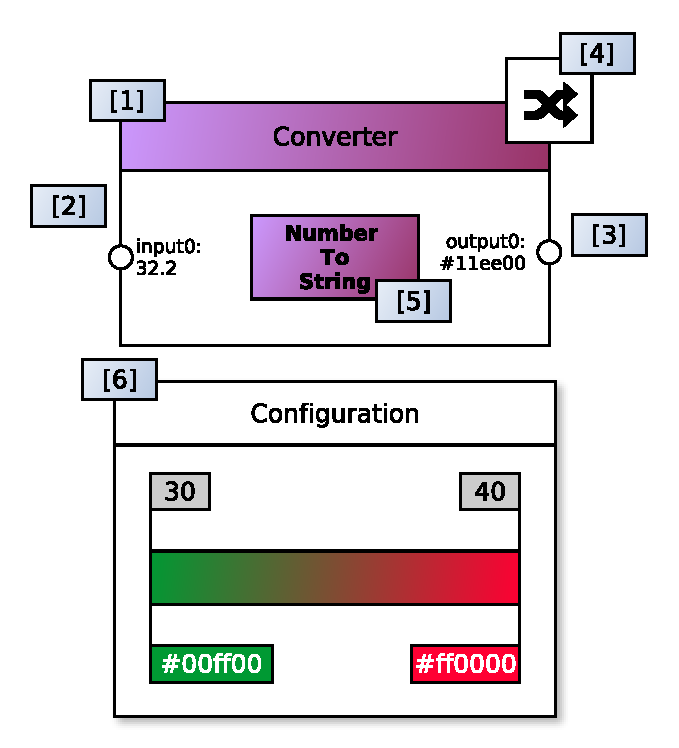
\includegraphics[width=1\linewidth]{bilder/Anhang/instanceconverterfunctionnode.pdf}
  \caption{Converter-Knoten: Bildet einen Definitionsbereich in einen Wertebereich ab.}
  \label{fig:actorgeneric}
\end{subfigure}%
\begin{subfigure}{.5\textwidth}
  \centering
  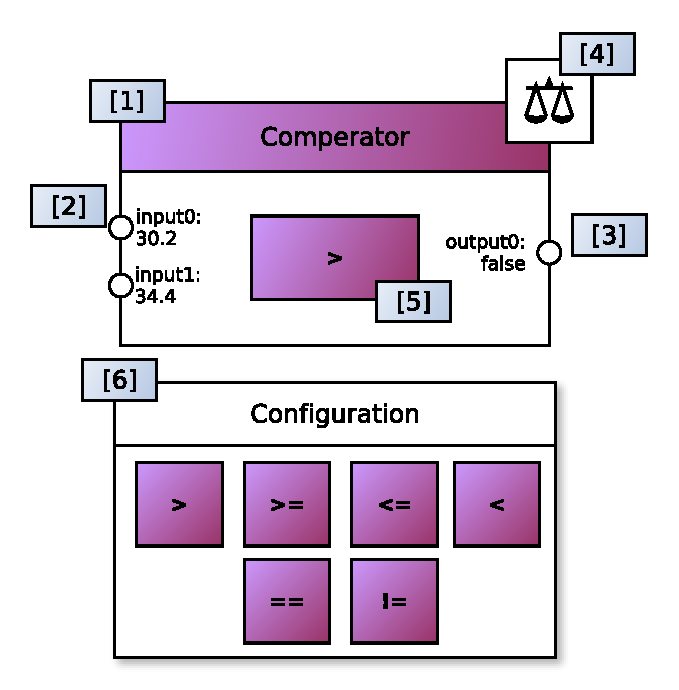
\includegraphics[width=1\linewidth]{bilder/Anhang/instancecomperatorfunctionnode.pdf}
  \caption{Comperator-Knoten: Vergleicht zwei \texttt{Number}-Werte und gibt einen Wahrheitswert weiter.}
  \label{fig:actorled}
\end{subfigure}

\begin{subfigure}{.5\textwidth}
  \centering
  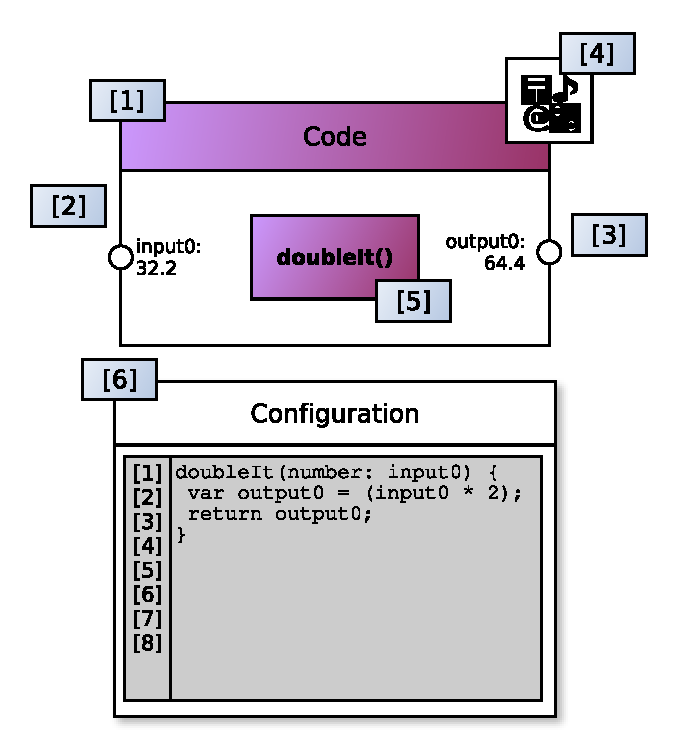
\includegraphics[width=1\linewidth]{bilder/Anhang/instancecodefunctionnode.pdf}
  \caption{Code-Knoten: Verarbeitet Daten anhand eines benutzerdefinierten Javascript-Programmcodes.}
  \label{fig:actorgeneric}
\end{subfigure}%
\begin{subfigure}{.5\textwidth}
  \centering
  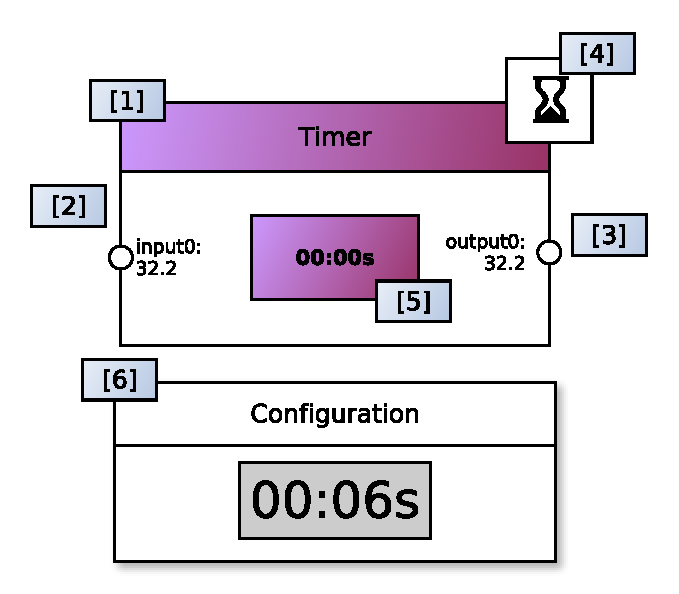
\includegraphics[width=1\linewidth]{bilder/Anhang/instancetimerfunctionnode.pdf}
  \caption{Timer-Knoten: Sendet das Eingangsignal nach einer benutzerdefinierten Zeitspanne weiter. [5] zeigt den momentanen Zustand des Timers an.}
  \label{fig:actorled}
\end{subfigure}




    \caption{Sammlung von verschiedenen Funktionsknoten. [1] Identifikationsleiste [2] Input-Schnittstellen [3] Output-Schnittstellen [4] Knoten-Indikator [5] Deskriptor [6] Knoten-Konfiguration}
    \label{fig:actornodes}
\end{figure}

\end{document}
